%; whizzy paragraph
%; whizzy-paragraph "^\\\\dancersection"
% -initex iniptex -latex platex -format platex -bibtex jbibtex -fmt fmt
% 以上 whizzytex を使用する場合の設定。

%     Tokyo Debian Meeting resources
%     Kansai Debian Meeting resources
%     Copyright (C) 2011 Junichi Uekawa
%     Copyright (C) 2011 Nobuhiro Iwamatsu

%     This program is free software; you can redistribute it and/or modify
%     it under the terms of the GNU General Public License as published by
%     the Free Software Foundation; either version 2 of the License, or
%     (at your option) any later version.

%     This program is distributed in the hope that it will be useful,
%     but WITHOUT ANY WARRANTY; without even the implied warranty of
%     MERCHANTABILITY or FITNESS FOR A PARTICULAR PURPOSE.  See the
%     GNU General Public License for more details.

%     You should have received a copy of the GNU General Public License
%     along with this program; if not, write to the Free Software
%     Foundation, Inc., 51 Franklin St, Fifth Floor, Boston, MA  02110-1301 USA

%  preview (shell-command (concat "evince " (replace-regexp-in-string "tex$" "pdf"(buffer-file-name)) "&"))
% 画像ファイルを処理するためにはebbを利用してboundingboxを作成。
%(shell-command "cd image2011-natsu; ebb *.png")

% progress memo:
% 2010/12-2011/05がマージ対象、関西は2010/12-2011/05(仮)
% イベント等でない場合は理由を書くこと。
% 必要な変更点は FIXME で記録しています。

%%ここからヘッダ開始。

\documentclass[mingoth,a4paper]{jsarticle}
\usepackage{monthlyreport}
\usepackage{supertabular}

% section の代わりの環境 -- 改訂する。
\renewcommand{\dancersection}[2]{%
\newpage
Deb専(旧あんどきゅめんてっど でびあん)2011年夏号
%
% top line
\vspace{0.1mm}\\
{\color{dancerdarkblue}\rule{\hsize}{2mm}}

%
% middle text
%
\begin{minipage}[t]{0.6\hsize}
\color{dancerdarkblue}
\vspace{1cm}
\section{#1}
\hfill{}#2\\
\end{minipage}
\begin{minipage}[t]{0.4\hsize}
\vspace{-2cm}
\hfill{}
\includegraphics[height=8cm]{image200502/openlogo-nd.eps}\\
\vspace{-5cm}
\end{minipage}
%
% bottom line
{\color{dancerlightblue}\rule{0.66\hsize}{2mm}}
%
\vspace{2cm}
}
% end of dancersection.

\begin{document}

\begin{titlepage}
\thispagestyle{empty}

\vspace*{-2cm}
Deb専(旧あんどきゅめんてっど でびあん) 2011年夏号\\
\hspace*{-2cm}

\includegraphics[height=210mm,angle=270]{image2011-natsu/debsen.pdf}\\
\hfill 2011年08月13日 初版発行

\rotatebox{10}{\fontsize{32}{32} {\gt 東京エリアDebian勉強会}}

\rotatebox{10}{\fontsize{32}{32} {\gt 関西Debian勉強会} }

\vspace*{-2cm}
\hfill{}
\includegraphics[height=6cm]{image200502/openlogo-nd.eps}
\end{titlepage}

\newpage
\thispagestyle{empty}\mbox{}
\newpage

\setcounter{page}{1}
\begin{minipage}[]{0.2\hsize}
 \definecolor{titleback}{gray}{0.9}
 \colorbox{dancerlightblue}{\rotatebox{90}{\fontsize{80}{80}
{\gt \color{dancerdarkblue}デビアン勉強会} }}
\end{minipage}
\begin{minipage}[]{0.8\hsize}
\hrule
\vspace{1mm}
\hrule
\setcounter{tocdepth}{1}
{\small
 \tableofcontents}
\vspace{1mm}
\hrule
\vspace{3cm}

\end{minipage}

% FIXME: 本文を追加すること。
%-------------------------------------------------------------------------------
\dancersection{Introduction}{上川 純一, 山下 尊也}
%-------------------------------------------------------------------------------

\subsection{東京エリアDebian勉強会}

 Debian勉強会へようこそ。これからDebianの世界にあしを踏み入れると
 いう方も、すでにどっぷりとつかっているという方も、月に一回Debianについ
 て語りませんか?

 Debian勉強会の目的は下記です。

\begin{itemize}
 \item \underline{Debian Developer} (開発者)の育成。
 \item 日本語での「\underline{開発に関する情報}」を整理してまとめ、アップデートする。
 \item \underline{場}の提供。
 \begin{itemize}
  \item 普段ばらばらな場所にいる人々が face-to-face で出会える場を提供
	する。
  \item Debian のためになることを語る場を提供する。
  \item Debianについて語る場を提供する。
 \end{itemize}
\end{itemize}

 Debianの勉強会ということで究極的には参加者全員がDebian Packageをがりがり
 と作るスーパーハッカーになった姿を妄想しています。情報の共有・活用を通し
 て Debianの今後の能動的な展開への土台として、「場」としての空間を提供す
 るのが目的です。

\subsection{関西 Debian 勉強会}

 関西 Debian 勉強会はDebian GNU/Linux のさまざ
 まなトピック(新しいパッケージ、Debian 特有の機能の仕組、Debian 界隈で起
 こった出来事、などなど)について話し合う会です。

 目的として次の三つを考えています。
 \begin{itemize}
  \item MLや掲示板ではなく、直接顔を合わせる事での情報交換の促進
  \item 定期的に集まれる場所
  \item 資料の作成
 \end{itemize}

 それでは、楽しい一時をお楽しみ下さい。

%-------------------------------------------------------------------------------
% end of header
%-------------------------------------------------------------------------------



%-------------------------------------------------------------------------------
\dancersection{「フリー」って、どういうこと?}{木下 達也}
%-------------------------------------------------------------------------------
\index{フリー}
\index{フリーソフトウェア}

\subsection{フリーソフトウェアとは}

Debianはフリーソフトウェアで構成されたオペレーティングシステムです。
ここで言う「フリー」とは「無料」ではなく「自由」を意味しています。

Free Software Foundation (FSF)による『フリーソフトウェアの定義』
では次のように説明されています。

\begin{quote}
「フリーソフトウェア」のフリーとはそのソフトウェアの
ユーザに与えられる4種類の自由を意味しています。

\begin{itemize}
 \item 目的を問わず、プログラムを実行する自由(第0の自由)。

 \item プログラムがどのように動作しているか研究し、そのプログラムに あなたの必要に応じて修正を加え、採り入れる自由(第1の自由)。ソースコードが入手可能であることはこの前提条件となります。

 \item 身近な人を助けられるよう、コピーを再頒布する自由(第2の自由)。

 \item プログラムを改良し、コミュニティ全体がその恩恵を受けられるよう あなたの改良点を公衆に発表する自由(第3の自由)。ソースコードが入手可能であることはここでも前提条件となります。

\end{itemize}

(\url{http://www.gnu.org/philosophy/free-sw.ja.html})
\end{quote}

\subsection{著作権とライセンス}

著作物には、基本的に著作者に対して著作権が発生しており、
著作物を変更したりコピーして配ったりするには、
著作者からの許可(ライセンス)が必要になります。

フリーかどうかを判定する際には、
変更や配布が許可されているか、
それらに付随する制約はどうか、
といった点を確認します。

そのほかに、特許、商標など個別の事情についても検討します。

\subsection{Debianフリーソフトウェアガイドライン}
\index{DFSG}
\index{Debianフリーソフトウェアガイドライン}

ある著作物がフリーかどうか、Debianの構成要素として適しているかどうかを
判定する際の基準、それがDebianフリーソフトウェアガイドライン(DFSG)です。

\begin{quote}
\begin{enumerate}
 \item 自由な再配布

 \item ソースコード

 \item 派生ソフトウェア

 \item 原作者によるソースコードの整合性維持

 \item すべての個人、団体の平等

 \item 目標分野の平等

 \item ライセンスの配布

 \item ライセンスはDebianに限定されない

 \item ライセンスは他のソフトウエアを侵害しない

 \item フリーなライセンスの例

\end{enumerate}

(\url{http://www.debian.org/social_contract#guidelines})
\end{quote}

DFSGの各条項について簡単に説明します。

\begin{enumerate}
 \item 自由な再配布 (Free Redistribution)

有償・無償を問わず、別途の許可を必要とすることなく、
プログラムを複数まとめて配布できます。

 \item ソースコード (Source Code)

ソースコード(変更に適した形式)が必要です。
実行形式だけでなくソースコードでも配布できます。

 \item 派生ソフトウェア (Derived Works)

同様のライセンスで変更版を配布できます。

 \item 原作者によるソースコードの整合性維持
   (Integrity of The Author's Source Code)

変更版のソースコードを配布する場合に、
元のソースコードと差分(パッチ)という形式のみ許可
という制約は許容します。ただし非推奨です。

 \item すべての個人、団体の平等
   (No Discrimination Against Persons or Groups)

いかなる個人・団体も差別せずに許可します。

 \item 目標分野の平等
   (No Discrimination Against Fields of Endeavor)

商用・非商用など、用途を制限しません。

 \item ライセンスの配布
   (Distribution of License)

ライセンスは、再配布されたすべての人々に、
別途の許可を必要とすることなく適用されます。

 \item ライセンスはDebianに限定されない
   (License Must Not Be Specific to Debian)

Debianの一部としてのみの許可ではなく、
他のシステムにも適用できるようにします。

 \item ライセンスは他のソフトウエアを侵害しない
   (License Must Not Contaminate Other Software)

たとえば、同じ媒体で配布されるソフトウエアすべてが
フリーであることを要求しないようにします。

 \item フリーなライセンスの例
   (Example Licenses)

GNU General Public License (GPL), BSD License, Artistic Licenseが
例として挙げられています。

\end{enumerate}

\subsection{オープンソースの定義}
\index{オープンソース}
Open Source Initiative (OSI)による『オープンソースの定義』(OSD)は
DFSGを元に作られました。何度か改訂されていますが、
現状でも内容はDFSGとほぼ同等のものです。

ここでは、一見して異なるOSD第10条についてのみ説明します。

\begin{quote}
10. ライセンスは技術中立的でなければならない

(\url{http://opensource.jp/osd/osd-japanese.html})
\end{quote}

たとえば、GUI環境で「同意する」ボタンを押すことが
必須であってはならない、ということになります。
内容としてはDFSG/OSDの第7条に含まれているものとも言えそうですが、
OSDでは、いわゆるクリックラップについて、この条項で特に注意を促しています。

\subsection{コピーレフト}

コピーレフトとは、著作物やその変更版について、
フリーであることを要求するための方法のことです。

GNU GPLは代表的なコピーレフトライセンスです。
GNU GPLで配布されるソフトウェアは、その変更版の配布についてもGNU GPLが適用され、
フリーソフトウェアであり続けます。

著作物全体への適用が「弱い」コピーレフトライセンスもあります。
たとえば、GNU Lesser General Public License (LGPL)で配布されるライブラリは、
リンクするプログラム全体についてはコピーレフトが適用されません。
そのほかに、Mozilla Public License (MPL)、
Eclipse Public License (EPL)、
Common Development and Distribution License (CDDL)など、
ファイル・モジュール単位でのコピーレフトライセンスもあります。

\subsection{ライセンスの互換性}

複数の著作物を組み合わせて一つの著作物にする場合、
それぞれのライセンスによる要求が矛盾しないかどうか、
互換性が問題になることがあります。

たとえば、CDDLではGNU GPLとは違った要求をしているので、
GNU GPLで配布されるソフトウェアとCDDLで配布されるソフトウェアを
組み合わせた著作物は配布できません。

ライセンスの非互換を回避するには、
複数のライセンスを適用する(デュアルライセンス)、
例外条項を設ける、
単純で何でも許可するようなライセンスにする、
といった方法があります。

\subsection{ASPループホール}

GNU GPLには、アプリケーションサービスプロバイダ(ASP)の
抜け穴(loophole)が存在することが知られています。

手元のコンピュータではなく「あちら側」のコンピュータで
実行されるウェブアプリケーションの場合、
そのウェブアプリケーションがGNU GPLで配布された
ソフトウェアを含んでいたとしても、
ネットワークユーザーにソースコード込みで再配布
されるわけではありません。

その抜け穴をふさぐためのライセンスが
GNU Affero General Public License (AGPL)です。
ネットワークユーザーへのソースコード提供を求める条文が
GNU GPLに加えられたものになっています。

\subsection{自由と協力}

なぜソフトウェアをフリーにするのでしょうか。
フリーソフトウェア、オープンソースの関係者それぞれに様々な思惑があることと思いますが、
ここでは一つの考えを挙げておきます。

個人の自由を促進し人々が協力し合うこと、
自分のためにみんなのために実践できること、
それがソフトウェアに関することなのであれば、
フリーソフトウェアがよく似合います。

Debianプロジェクトはフリーソフトウェアを強く支持しています。

Happy Hacking!

\subsection{参考資料}

\begin{thebibliography}{0}
 \bibitem{free} フリーとは何だろう? あるいはフリーソフトウェアとは何を意味
	 するのか?,
\url{http://www.debian.org/intro/free.ja.html},
\url{http://www.debian.org/intro/free.en.html}

 \bibitem{freesw} フリーソフトウェアの定義,
\url{http://www.gnu.org/philosophy/free-sw.ja.html},
\url{http://www.gnu.org/philosophy/free-sw.html}

 \bibitem{socialcontract} Debian 社会契約 / Debian フリーソフトウェアガイドライン (DFSG),
\url{http://www.debian.org/social_contract.ja.html},
\url{http://www.debian.org/social_contract.en.html}

 \bibitem{licenses} Debian -- ライセンス情報,
\url{http://www.debian.org/legal/licenses/index.ja.html},
\url{http://www.debian.org/legal/licenses/index.en.html}

 \bibitem{dfsg} DFSG and Software License FAQ (Draft),
\url{http://people.debian.org/~bap/dfsg-faq.html}

 \bibitem{opensource} オープンソースの定義,
\url{http://opensource.jp/osd/osd-japanese.html},
\url{http://opensource.org/docs/osd}

 \bibitem{opensourcelicenses} Open Source Licenses,
\url{http://opensource.org/licenses/index.html}

 \bibitem{copyleft} コピーレフトって何?,
\url{http://www.gnu.org/copyleft/copyleft.ja.html},
\url{http://www.gnu.org/copyleft/copyleft.html}

 \bibitem{licenseslist} さまざまなライセンスとそれらについての解説,
\url{http://www.gnu.org/licenses/license-list.ja.html},
\url{http://www.gnu.org/licenses/license-list.html}

 \bibitem{gplfaq} GNU GPLに関して良く聞かれる質問,
\url{http://www.gnu.org/licenses/gpl-faq.ja.html},
\url{http://www.gnu.org/licenses/gpl-faq.html}

 \bibitem{aboutdebian} Debian について
\url{http://www.debian.org/intro/about.ja.html},
\url{http://www.debian.org/intro/about.en.html}

\end{thebibliography}

%-------------------------------------------------------------------------------
\dancersection{Squeezeの変更点をみんなで見てみよう}{倉敷 悟}
%-------------------------------------------------------------------------------
\index{squeeze}

\subsection{Squeezeの情報源}

主な情報源としては下記のものがあります。
このうち、リリースノートの読み方を簡単に紹介しつつ、目立った変更をざっく
り眺めていこうと思います。

\begin{itemize}
 \item Debian -- ニュース -- Debian 6.0 ``Squeeze'' released:
       \url{http://www.debian.org/News/2011/20110205a}
 \item Debian GNU/Linux 6.0 (squeeze) リリースノート (32 ビット PC 用):
       \url{http://www.debian.org/releases/stable/i386/release-notes/index.ja.html}
 \item NewInSqueeze - Debian Wiki: \url{http://wiki.debian.org/NewInSqueeze}
\end{itemize}

\subsection{Debian リリースノートの読み方}

% 読み方、なんて題名にしてますが、まさか読んでない……なんてことは……
% まさかね。

\subsubsection{大まかな構造}

さて、リリースノートは、構造はほぼ決まっていて、各リリースでの違いだけが反映
されていくようになっています。

その章立ては次の通りです。これは、原文自体がこのような形で分割されている
ので、基本的には今後のリリースでも踏襲されると思います。

\begin{multicols}{2}
 \begin{itemize}
 \item 前置き
 \item 最新情報
 \item インストーラの変更点
 \item アップグレード
 \item 問題点
 \item 参照情報
 \item oldstable での事前準備
 \item 目録
 \end{itemize}
\end{multicols}

まずは、「最新情報」をざっくり読んだあと、「問題点」にしっかり目を通すの
が大切です。結局、squeeze で何が変化してどうなったのか、という情報は
ここに集っているからです。

「インストーラの変更点」は、新規にインストールする人は一応見ておきましょ
う。といっても、最近のインストーラは、わりと「見ればわかる」ようになって
いるので、インストールするだけなら読まなくても問題になることは少ないと
思います。
ちなみに、今回からは、最新のインストーラが以前のバージョンもインストール
できるようになったらしいです。最新のインストーラで woody とか sarge を
入れたらどんな (目もあてられない) ことになるのか、興味深いですね。

「アップグレード」と「oldstable での事前準備」は、インストーラを使わずに
以前のリリースから更新する人はとにかく必読です。これは言わば、
「既に踏まれた地雷」を考慮に入れたアップグレード作業の手順書です。
従って、ここに書かれた内容にハマってしまうというのは、なんというか
(政治的に正しくない言葉をお好みで) ということになってしまいますので
注意してください。

ちなみに、「なんだ用語集か」と思って見過ごしてしまいがちなのですが、
「目録」のページには、パッケージ名からの逆引きインデックスが含まれて
いたりしますので、「あのパッケージに何か (わざわざリリースノートで
触れないといけないような) 変化があるかな」といった見方をすることも
できたりします。一度くらいは見てみるといいかも知れません。

\subsubsection{どのように書かれるか}
さて、最初に書いた通り、リリースノートは、これまでの文章に随時継ぎ足し
たり削ったりして、秘伝のタレのように作られていきます。

ここで、「前置き」の部分に着目してみましょう。
そういった変更は、DDP (Debian Documentation Project) のメンバーが
適宜行う他、主に BTS の release-notes に対するリクエストへの対応と
してもなされます。あるパッケージのバグについてやりとりしている中で、
「あ、これはリリースノートに書いとかないと」という流れになることも
あります。

既に書いた「既に踏まれた地雷」はこういう形で集められたものですので、
残念ながら網羅性があるわけではありません。皆さんも、何か新しい地雷を
踏んじゃったなー、という時は、遠慮なく BTS へ報告してください (英語で)。

ここで注意が必要なのは、こういった BTS の動きもあって、
「リリースノートはリリースされた後にも更新される場合がある」
ということです。今自分が読んでいるのが最新かどうか、ということには
ちょっと注意しておくといいでしょう。
\url{http://svn.debian.org/viewsvn/ddp/manuals/trunk/release-otes/en/}
を見て、各ファイルの最終更新日をチェックするのがお手軽です。

翻訳が追いついていないこともあるので、その場合は頑張って英語で読んだ後、
debian-doc あたりに原文更新を通知しましょう。翻訳済みのパッチも歓迎され
ます。

\subsubsection{ともあれ Squeeze になった後}

リリースノートの「前置き」でも書かれていますが、基本的に、各パッケージ毎
の些細な変更はわざわざリリースノートに書かれたりしません。

普段使いのパッケージについては、とりあえず基本に立ち帰って、
「/usr/share/doc/パッケージ名」に README.Debian や NEWS.Debian が
追加されたり更新されたりしていないか、確認しておくようにしましょう。

おっかしーなー、想定と違う動き方をするなー、と思って散々ぐぐりまくった
あげくに NEWS.Debian にちゃんと書いてあった、というのはよくある話です。

\subsection{システムのコア部分の変更}
SqueezeになってLinuxカーネルとシステム起動部分に大きな変更がありました。

Linuxカーネルでは、カーネルにバイナリの形で含まれていた含まれていたファー
ムウェアが分離され、non-freeセクションに移動されました。
これによって、Debian の main セクションにある linux カーネルイメージは
完全にフリーになりました.
%
移動されたnon-freeのファームウェアにはAMD RadeonとBroadcomのファームウェ
アなどが入っており、NICが使えない、インストール後にXが起動しないなどの影
響が考えられます。

インストール中にnon-freeのファームウェアを読み込ませるには、
\url{http://cdimage.debian.org/cdimage/unofficial/non-free/firmware/}から
ファームウェアをダウンロードし、あらかじめUSBメモリなどに展開しておき、イ
ンストーラの指示に従って読み込ませます。
%
Debianインストール後にnon-freeのファームウェアをインストールするには、
apt-lineのnon-freeセクションを有効にして、firmware-linuxパッケージをイン
ストールします。(依存関係でfirmware-linux-free とfirmware-linux-non-free
の二つがインストールされます。)

システムの起動では、起動シーケンスが依存関係ベース(insserv)になり、デーモ
ンが並列起動されるようになりました。

デーモンの並列起動で問題が出た場合は、/etc/default/rcSに
「CONCURRENCY=none」と設定すると無効にできます。(insservはsysv-rcパッケー
ジが依存しているので残念ながら外すことはできません。)

\subsection{パッケージまわり}

``libs''、``network''などのパッケージセクションが分割された一方で、
``embedded''、``haskell''、``video'' などの新しいセクションが追加されました。
実際のところ、debian を単に使うだけなら、セクションは余り意識しなくても
さほど困らないので、開発者向けの変更点と言えるかもしれません。

今までbackports.orgで提供されていたバックポートされたパッケージが、
backports.debian.orgから提供されるようになりました。
debian.org の公式サービスへと格上げされたため、これまでよりは敷居が下がっ
て使いやすくなっっと思います。

volatile.debian.orgで提供されていたパッケージが、stable-updatesという形
で提供されるように変更されました。
アンチウィルス系など、リリース後も継続してデータの更新が必要な種類のパッ
ケージが volatile で提供されていましたが、パッケージ数も少なく、ほぼ
機能していない状態でした。これが stable-updates となって状況が改善されれ
ばいいですね。

いろいろと細かい変更のある APT まわりですが、まずは推奨(Recommends)パッ
ケージを全部自動的にインストールされるようなっている、という点おおさえて
おきましょう。RedHat を思わせる勢いであれもこれも入ってくるので、ストイッ
クにいきたい人は、-R オプションを活用してください。

また、apt-get と aptitude の位置付けがまた変更されています。
コマンドラインでポンと投げる場合は apt-get を使います。また、ディストリ
ビューションのアップグレードにも、aptitude ではなく apt-getを使うことが
推奨されています。
aptitude は引数なしで起動して、コンソール GUI で使うもの、ということにな
るようです。

\subsection{ハードウェアまわり}

Squeezeのハードウェア周辺の対応を見ていきましょう。

対応アーキテクチャですが、一番目を引くのはテクノロジープレビューという形
ですが、LinuxカーネルではなくFreeBSDカーネルを使った、kfreebsd-amd64と
kfreebsd-i386の追加でしょう。kFreeBSDについては前回、杉本さんの資料もご覧
ください。

そのほかには、LennyまでサポートされていたHP PA-RISC ('hppa')、Alpha
('alpha')、ARM ('arm')アーキテクチャが廃止になり、対応アーキテクチャは、
32ビットPC ('i386')、64ビットPC ('amd64')、PowerPC ('powerpc')、SPARC
('sparc')、Intel Itanium ('ia64')、ARM EABI ('armel')、MIPS ('mips' (ビッ
グエンディアン)、'mipsel' (リトルエンディアン))、S/390 ('s390')の9つ+2の
11種類のサポートになりました。\footnote{sh は wheezy?}

X関係のサポートを見ると、Intel, AMD, NVIDIAのメジャーなグラフィックチップ
においてカーネル内でグラフィック設定を行う、カーネルモードセッティング
(KMS)が有効化されています。

これらによりXの起動が早くなったり、サスペンド・レジュームでXが死ななくな
るなど良い面もある反面、コンソール画面の文字が出なくなったりするなどの影
響もあります。\\
その場合は\texttt{/etc/modprobe.d/(i915|radeon|nouveau)-kms.conf}の
設定を変更する必要があります。
\footnote{\url{http://wiki.debian.org/KernelModesetting}}

細かいところではXとコンソールのキーボード設定が統一化されました。

\texttt{/etc/default/keyboard}にキーボードの設定をしておくと、コンソールとXの設定
は上書きされて同じ設定になります。

lennyから基本的にxorg.confは使わなくなったので影響は少ないと思いますが、
xorg.confを書いている人は注意が必要です。

%-------------------------------------------------------------------------------
\dancersection{Squeezeをみんなインストールした結果を語る会}{まえだ こうへい}
%-------------------------------------------------------------------------------
\index{squeeze}

事前課題ではSqueezeになってうれしい点、変わった点を挙げてもらいましたが、
実際にインストールしてみた結果を語りましょう。

\subsection{インストールした機器}

\begin{table}[H]
 \begin{center}
  \begin{tabular}{|p{10em}|p{15em}|p{15em}|}
   \hline
   メーカー & 機種名 & 誰 \\
   \hline
   HP & MicroServer & まえだ\\
   \hline
  \end{tabular}
 \end{center}
\end{table}

\subsection{インストールで困ったこと}

\begin{table}[H]
 \begin{center}
  \begin{tabular}{|p{15em}|p{10em}|p{15em}|p{5em}|}
   \hline
   困ったこと & 解決したか? & 解決方法 & 担当 \\
   \hline
   プリンタの設定に少々悩んだ(詳細忘れた)& 解決? & 解決方法を思い出して情報共有す
	   る。 & キタハラ\\
   \hline
  \end{tabular}
 \end{center}
\end{table}

\subsection{改善した方が良いと思ったこと}

\begin{table}[H]
 \begin{center}
  \begin{tabular}{|p{15em}|p{12em}|p{15em}|p{3em}|}
   \hline
   改善した方良いと思ったこと & Sidでも再現するか? & あなたの宣言 & 担
   当 \\
   \hline
   libvirt のnwfilterの設定によって、自分で設定しているiptablesのルール
   が上書きされる & 未検証 & /etc/libvirt/nwfilterにルールを追加するか、その
	   下をすべて削除して自分で作っているスクリプトに集約する。前者
	   はルールの順番がよく分からないので仕組みを理解する。 & まえだ\\
   \hline
   Klipperの挙動が変わり、中ボタンでのペースが面倒になった。& & 「クリップ
	   ボードのアクションを有効にする」で解決するか確認する。しなけ
	   れば改善案を考えてBTS。 & 山本\\
   \hline
   心残りがあること & そのままSidにある? & すっきり解決する。 & 岩松 \\
   \hline
   Debian InstallerでLVMを一度設定すると削除できない。& Yes。シェルモー
       ドでlvremove, vgremove, pvremoveすれば削除できる。 & メニューから
	   も普通に削除できた方が良いんじゃね。 & まえだ \\
   \hline
  \end{tabular}
 \end{center}
\end{table}

%-------------------------------------------------------------------------------
\dancersection{Debian のドキュメントをみてみよう}{かわだ てつたろう}
%-------------------------------------------------------------------------------
\index{doc-base}
\subsection{はじめに}
Debian プロジェクトはユーザに向けたドキュメントを提供しています。ドキュ
メントパッケージを管理する doc-base のクライアントとともに Debian を使っ
ていくうえで有用な Debian 固有のドキュメントをいくつか紹介します。


\subsection{doc-base}
doc-base とは Debian システムにインストールされたドキュメントを管理す
るユーティリティとドキュメントのメタデータのデータベースを提供するパッ
ケージです。単なる man ページだけでなくオンラインドキュメントを提供す
る Debian パッケージはインストール時に doc-base に登録し、アンインストー
ル時に登録を解除することが推奨されています。\footnote{Debian Policy
 Manual: 9.10 Registering Documents using doc-base}
doc-base に登録されたメタデータを利用するクライアントとして dwww,
dhelp, doc-central などが提供されています。これらクライアントを利用す
ればドキュメントの検索、閲覧が容易に行えます。

\subsection{doc-base クライアント}
doc-base クライアントをいくつか紹介します。


\subsubsection{dwww}
\index{dwww}
dwww はウェブベースのドキュメントリーダです。

doc-base に登録されたドキュメント、man、info を参照することができます。
ドキュメントはインデックス化されており検索することができます。

\subsubsubsection{インストール}

apt を使用してインストールするだけですが info を表示する info2www の設
定が少し必要です。

info2www のシンボリックリンクを作成して info2www をドキュメントルート
下(ここでは /var/www)に公開させます。info2www を公開させなくても動作し
ますが info を表示する場合に画像などが表示されません。
\footnote{/usr/share/doc/info2www/README.Debian 参照}

またインストール直後はインデックスの作成に少し時間がかかりますのでしば
らく待ってから dwww を使用してください。

\begin{commandline}
$ sudo aptitude install dwww
$ sudo ln -s /var/lib/info2www /var/www/info2www
\end{commandline}

\subsubsubsection{使い方}

WEB ブラウザで \url{http://localhost/dwww} にアクセスするかコマンドラ
インで dwww と実行してください。ブラウザに dwww のホームが表示されます。
後は WEB ブラウジングするようにリンクを辿るか入力フォームにキーワード
を入力して検索を行ない目的のドキュメントを探してください。残念ながら日
本語での検索はできません。

検索はコマンドラインから行なうこともできます。例えば debian という検索
をコマンドラインから行ないたい場合は以下のように実行すれば WEB ブラウ
ザに debian と検索した結果が表示されます。

\begin{commandline}
  $ dwww debian
\end{commandline}


\subsubsection{dhelp}
\index{dhelp}

dhelp はウェブベースのドキュメントリーダです。

WEB ブラウザから doc-base に登録されたドキュメントを参照することができ
ます。ドキュメントはインデックス化されており検索することができます。

\subsubsubsection{インストール}

apt を使用してインストールするだけです。dhelp は WEB サーバを必要とし
ていませんのでここで WEB サーバはインストールされません。インストール
直後はインデックスの作成に少し時間がかかりますのでしばらく待ってから
dhelp を使用してください。

\begin{commandline}
  $ sudo aptitude install dhelp
\end{commandline}
%$ -- for emacs

\subsubsubsection{使い方}

WEB ブラウザで \url{file://localhost/usr/share/doc/HTML/index.html} に
アクセスするかコマンドラインで dhelp と実行してください。ブラウザに
dhelp のホームが表示されます。後は WEB ブラウジングするようにリンクを
辿ってドキュメントを探してください。この状態では info pages, man pages
の参照、ブラウザからの検索を行なうことはできません。

検索はコマンドラインから行なうことになります。例えば debian という検索
をコマンドラインから行ないたい場合は以下のように実行すれば WEB ブラウ
ザに debian と検索した結果が表示されます。残念ながら日本語での検索はで
きません。

\begin{commandline}
  $ dhelp debian
\end{commandline}
%$ -- for emacs

\subsubsubsection{WEB サーバの導入}

WEB サーバを必要としないのは一つのメリットですが制限もあり不便ですので
WEB サーバをインストールして WEB ブラウザからの検索、info と man の参
照ができるようにします。dhelp パッケージが Suggests しているパッケージ
を参考に apache2 と info2www, man2html を追加インストールします。先と
同様に info2www の設定を少し行ないます。

\begin{commandline}
  $ sudo aptitude install apache2 info2www man2html
  $ sudo ln -s /var/lib/info2www /var/www/info2www
\end{commandline}

これで WEB サーバを経由で dhelp を使用できるようになりました。
dhelp コマンドの結果は WEB サーバ経由で表示されるようになりますが WEB
ブラウザに直接アドレスを入力する場合はアドレスを
\url{http://localhost/doc/HTML/index.html} に変更してください。


\subsubsection{doc-central}
\index{doc-central}

doc-central はウェブベースのシンプルなドキュメントリーダです。

WEB ブラウザから doc-base に登録されたドキュメントを参照することができ
ます。doc-central はドキュメントをインデックス化しませんが doc-base の
メタデータに登録されたドキュメント名、作者、概要を対象として検索するこ
とができます。man は参照することができません。

\subsubsubsection{インストール}

apt を使用してインストールするだけですが info2www の設定が少し必要です。

\begin{commandline}
  $ sudo aptitude install doc-central
  $ sudo ln -s /var/lib/info2www /var/www/info2www
\end{commandline}

\subsubsubsection{使い方}

WEB ブラウザで \url{http://localhost/dc/} にアクセスするかコマンドライ
ンで doccentral と実行してください。doc-central ではなく doccentral で
す。ブラウザに Doc-Central のホームが表示されます。後は WEB ブラウジン
グするようにリンクを辿るか入力フォーム\footnote{左側フレームの最下部に
  あります}にキーワードを入力して検索を行ない目的のドキュメントを探し
てください。

検索はコマンドラインから行なうこともできます。例えば debian という検索
をコマンドラインから行ないたい場合は以下のように実行すれば WEB ブラウ
ザに debian と検索した結果が表示されます。

\begin{commandline}
  $ doccentral debian
\end{commandline}


\subsubsection{その他に}

\subsubsubsection{Yelp}
\index{yelp}

Yelp は Gnome のヘルプブラウザです。

Yelp からは man と info そして Gnome のヘルプが参照できますが各パッケー
ジのドキュメントは参照できません。

\subsubsubsection{khelpcenter}
\index{khelpcenter}

khelpcenter4 は KDE のヘルプセンタです。

khelpcenter4 からは man と KDE のヘルプが参照できますが info や各パッ
ケージのドキュメントは参照できません。

\subsection{The Debian Documention Project のドキュメント}
doc-base クライアントが使えるようになったところで、パッケージとして提
供されている The Debian Documention Project (DDP) のドキュメントをいく
つかざっとみていきます。

\subsubsection{doc-debian}
\index{doc-debian}
Debian の基礎となる Debian 社会契約や Debian フリーソフトウェアガイド
ラインといった Debian プロジェクトの基礎となる文書群です。


\subsubsection{installation-guide}
\index{installation-guide}

インストールガイドです。

squeeze では 12 種類のアーキテクチャ毎にパッケージが用意されています。
\footnote{squeeze では hppa のサポートが外れ 11 種類のアーキテクチャが
サポート対象ですが installation-guide-hppa パッケージが存在します。}
i386 アーキテクチャ用だとパッケージ名は installation-guide-i386 になり
ます。

初めて Debian をインストールする場合に参照することになるでしょう。
CD-ROM/DVD-ROM や USB メモリといったメディアからのインストール以外にも
debootstrap やネットブートを使用したインストール方法、preseed を利用し
たインストールの自動化についても説明されています。ちょっと違ったインス
トールをする場合にも参考になることが記載されています。

手早くインストールの流れを確認するだけなら「付録 A. インストール Howto」
を参照してください。もしもの場合に供えて「5.4. インストールプロセスの
  トラブルシューティング」も見ておくことをおすすめします。


\subsubsection{debian-reference}
\index{debian-reference}

Debian システムの広範な概論です。

日本語訳は debian-reference-ja として別パッケージで提供されています。

内容は大変多岐に渡りコンソールの基礎から Debian でのパッケージ管理、ネッ
トワーク設定、プログラミングまで扱っています。DDP の中でも最も充実した
ユーザマニュアルです。

Unix ライクなシステムを使った経験があまり無いのであればぜひ
「1. GNU/Linux チュートリアル」を参照してください。Debian のパッケージ
については「2. Debian パッケージ管理」で詳細に説明されています。
unstable を使いはじめようという時には「2.6. 壊れたシステムからの復元」
が手助けになるかもしれません。その他 Debian を使っている各局面にあわせ
て項目を参照してみるとよいでしょう。


\subsubsection{maint-guide}
\index{maint-guide}

新たにパッケージメンテナになろうという人向けの解説です。

「Debian 新メンテナガイド」、「Debian メンテナ入門」、
「ニューメンテナガイド」、「新規メンテナのためのガイド」などと呼ばれて
います。日本語訳は maint-guide-ja として別パッケージで提供されています。

gentoo パッケージを例にとってパッケージの作成、アップロード、更新手順
が説明されています。
内容の大半がパッケージ作成に割かれて詳しく説明されていますのでパッケー
ジメンテナになろうという人だけでなく、Debian のパッケージを作ってみよ
うと思う方も是非参照してください。


\subsubsection{developers-reference}
\index{developers-reference}

Debian 開発者向けのリファレンスです。

日本語訳は developers-reference-ja として提供されていますが翻訳途中で
す。

新規メンテナプロセスから始まり Debian Developer が使用できるリソース、
パッケージの扱い方が説明されています。特に技術的な事柄以外のパッケージ
化についてありとあらゆる情報が記載されています。
Debian Developer の活動の一部を垣間見られるドキュメントです。


\subsubsection{debian-policy}
\index{debian policy}

Debian ポリシーマニュアルとポリシーを補足する文書群です。

Debian ポリシーマニュアルには Debian パッケージの内部構造(アーカイブ構
成、パッケージの各書式など)やオペレーティングシステムとして必要な設計
部(ファイルシステムの階層構造、システムや各種プログラムの設定など)につ
いて記載されています。日々議論され更新されています。

日本語訳されたパッケージはありませんが Debian JP Project で Debian ポ
リシーマニュアル(Version 3.8.3.0)を翻訳したものが WEB で公開されていま
す。
\footnote{\url{http://www.debian.or.jp/community/devel/debian-policy-ja/policy.ja.html/}}
過去に東京エリア Debian 勉強会でとりあげられていますのでその資料も参考
にしてみてください。
\footnote{第 12, 13, 15 回東京エリア Debian 勉強会事前資料参照}


\subsubsection{その他}
\subsubsubsection{debian-faq}
Debian に関する FAQ がまとめられています。


\subsubsubsection{harden-doc}
Debian のセキュリティに関することをまとめたマニュアルです。システムの
セキュリティに関することからプロジェクトのセキュリティ取り組みについて
も記載されています。現在、日本語への翻訳が進められています。


\subsubsubsection{debian-refcard}
いわゆるリファレンスカードです。一枚の紙(A4 裏表)に重要なコマンドの一
覧や参考となる情報をまとめてあります。


\subsection{最後に}

ドキュメントは随時更新されており最新ドキュメントは  Debian のユーザ文
書\footnote{\url{http://www.debian.org/doc/}}にまとめられていますので
確認してみてください。ここにはパッケージになっていないドキュメント(例
えばリリースノートなど)もあります。
ドキュメントソースは Subversion で管理、公開されておりどなたでも確認す
ることができます。興味があればこちらも覗いてみてください。
\footnote{\url{http://www.debian.org/doc/cvs.ja.html}}

ドキュメントに間違いを見つけた場合は BTS するか、日本語訳に関すること
であれば \url{debian-doc@debian.or.jp} に報告するとよいでしょう。

また、The Debian Documention Project が提供するドキュメント以外にもソ
フトウェアのドキュメントパッケージがたくさんありますのでパッケージの
``doc'' セクションも覗いてみてください。

\subsection{参考資料}
\begin{itemize}
 \item Debian ユーザ文書: \url{http://www.debian.org/doc/}
 \item doc-base: \url{http://wiki.debian.org/doc-base/}
\end{itemize}

%-------------------------------------------------------------------------------
\dancersection{ハッカーに一歩近づく Tips:vi 編}{山下 康成}
\index{vi}
\subsection{はじめに}

vi は、初心者は初心者なりに使え、使い込めば使い込むほど味の出るエディタだということは皆さんご存じの通りかと思います。
皆さんも当たり前のように vi を使ってらっしゃると思いますが、さて、ハッカーのように vi を使いこなせてますでしょうか?
ハッカーに近づくために、vi 使いこなしのちょっとした Tips を紹介します。

\subsection{こんな経験ありませんか?}

\begin{verbatim}
    k
    ↑
h ← → l
    ↓
    j
\end{verbatim}

\begin{description}
  \item[w] 一語右へカーソルを移動
  \item[G] ファイルの末尾へカーソルを移動
  \item[x] 1文字消す
  \item[dd] 1行消す
  \item[etc] ……
\end{description}

こんな教え方するから、バラバラなコマンドを覚えないとならず、なかなか「使い込めば味の出る」ところまで行けないのでしょう。今日はもうちょっと体系立てて説明してみます

\subsection{コマンドを整理してみる}

\subsubsection{繰り返し回数−コマンド 型}

回数に続いてコマンドを入力すると、指定した回数繰り返されるコマンド。
5yy として5行コピーとかは良く使われる。

例:
\begin{description}
  \item[2l] 2文字分右にカーソルを移動する
  \item[2h] 2文字分右にカーソルを移動する
  \item[2x] 2文字消す
  \item[2X] カーソルの左の2文字を消す
  \item[2r] 2文字を次に入力する文字と置き換える
  \item[2\~] 2文字を英大文字 \textless - \textgreater 小文字を切り替える

  \item[3w] 3ワード右にカーソルを移動する
  \item[3W] 空白区切りで 3 ワード右にカーソルを移動する
  \item[3b] 3ワード左にカーソルを移動する
  \item[3B] 空白区切りで 3 ワード左にカーソルを移動する

  \item[4yy] 4行コピーする
  \item[4dd] 4行削除する

  \item[5p] 5回ペーストする
  \item[5P] カーソルの前に5回ペーストする
  \item[5i \textless string \textgreater [ESC]] カーソルの左に \textless string \textgreater を5回入力する
  \item[5I \textless string \textgreater [ESC]] 行頭に \textless string \textgreater を5回入力する
  \item[5a \textless string \textgreater [ESC]] カーソルの右に \textless string \textgreater を5回入力する
  \item[5A \textless string \textgreater [ESC]] 行末に \textless string \textgreater を5回入力する
  \item[5H] 画面上から5行目にカーソルを移動する
  \item[5L] 画面下から5行目にカーソルを移動する
\end{description}

\subsubsection{事前課題}

以下、それぞれどのようにキー操作をすれば良いか、
最も少ないキー操作を考えてください。
\begin{itemize}
  \item 現在行から最終行(の行頭)にカーソルを移動する
  → G
  \item 現在行から最終行までを消去する
  → dG
\item 現在行から最終行までをコピー(yank)する
   → yG
\item 現在行から最終行までを ``x'' 1文字で置き換える
   → cGx \textless ESC \textgreater
\end{itemize}

「カーソル移動」というコマンドが省略されていると考えれば、
[コマンド]G という形になっていることに気が付いていただいただろうか?


\subsubsection{コマンド−目的地 型}


コマンド:
\begin{description}
  \item[省略] 「目的地」にカーソル移動
    「カーソル移動」は「``目的地''までカーソルを移動する」ということ
  \item[d] 「目的地」までを削除
  \item[y] 「目的地」までをコピー
  \item[c] 「目的地」までを変更
\end{description}

例:
\begin{description}
\item[d3l] 3文字左まで削除
\item[c3w] 3ワードを変更

\item[d0] 行頭までを削除
\item[d\textasciicircum] 空白をのぞく行頭までを削除
\item[d\textdollar] 行末までを削除 (= D)

\item[y5j] 5行下までをコピー
\item[d\%] 対応するカッコまでを削除
\item[dgg] 先頭行までを削除

\item[d/\textless string \textgreater] ``string'' があるところまでを削除
\end{description}

\subsection{そのほかの便利な機能}

\subsubsection{名前つきバッファ}

例:
\begin{description}
\item["ayy] バッファ a に1行コピー
\item["by\textdollar] バッファ b に行末までをコピー

\item["ap] バッファ a をペースト
\item["bP] バッファ b をカーソルの前にペースト
\end{description}

\subsubsection{コマンドの実行結果を追加}
\begin{description}
\item[:r ! ls] ls の実行結果をカーソル位置に挿入
\end{description}

\subsection{最後に}

vi のコマンドは、バラバラのように見えて
\begin{itemize}
      \item 繰り返し回数−コマンド 型
      \item コマンド−目的地 型
\end{itemize}

と整理してみると、結構直行しているということがわかっていただけたかと思います。

皆さんの知ってるコマンドも、この型にあてはめてみると知らなかった用途が見えてきたのではないでしょうか。

vi を使いこなして、ハッカーに一歩近づこう!

%-------------------------------------------------------------------------------
\dancersection{Debian GNU/kFreeBSD で便利に暮らすための Tips}{杉本 典充}
%-------------------------------------------------------------------------------
\index{Debian GNU/kFreeBSD}

\subsection{Debian GNU/kFreeBSD について}
Debian GNU/kFreeBSD とは, Debian Project で開発しているオペレーティングシステムのひとつです. Squeeze にて技術プレビュー版としてリリースされることになっています. \footnote{\url{http://www.debian.org/ports/kfreebsd-gnu/}}

\subsubsection{Debian GNU/kFreeBSD の現状}
Debian GNU/kFreeBSD は現在次のような状況です.

\begin{itemize}
  \item カーネルは FreeBSD 8.1 ベースのものに一本化された. (7.3 カーネルは廃止).\footnote{2011年6月末現在、unstableでは8.2系カーネル、experimentalでは9.0系カーネルをベースに開発が行われています.}
  \item まだ Linux バイナリ互換機能は動かない模様. (linux.ko のロード自体に失敗する).\footnote{2011年6月末現在、まだ動作していません.}

\end{itemize}

\subsection{ZFS 環境下でリアルタイム系アプリケーションを使用する Tips}
\subsubsection{現象}
私の PC 環境では, sftp を実行してサーバから 1GB のファイルをダウンロードすると, audacious で再生中の MP3 ファイルが音飛びします. ディスクのアクセス LED は「消灯, 数秒間連続点灯, 消灯」を繰り返すようなディスクアクセスをしており, 音飛びは HDD LED が点灯中に発生します.

なお, PC の環境は以下です.

\begin{itemize}
  \item ノート PC の VAIO TZ. 2.5inch HDD (SATA150 接続) の 250GB.
  \item / は UFS, /home は ZFS としている.
  \item ZFS の設定で, 圧縮はしない (compression=off) 設定にしている.
  \item 再生する MP3 ファイルと sftp でダウンロードする 1GB のファイルは双方 ZFS 領域に読み書きする.
\end{itemize}

\subsubsection{原因の推定}
ディスクのアクセス LED が点灯しているときに MP3 ファイルの再生が音飛びするため, 1GB のファイルを書き込み中に MP3 ファイルの読み込みが行えなかったためと推測します.

そのため, 大きいファイルを書き込む場合はディスクへの連続書き込み時間を短くするように ZFS のパラメータを調整すれば現象は解決すると考えます.

ZFS のパラメータ設定については FreeBSD を使う人たちで研究されており, その結果が公開されています. \footnote{\url{http://wiki.freebsd.org/ZFSTuningGuide}}

\subsubsection{ZFS のパラメータを調整する}
ZFS のパラメータを表示するには ``sysctl'' コマンドを使用します.
今回調整するパラメータは \verb!vfs.zfs.arc_max!のため, 現在の値を確認します.

\begin{commandline}
$ sysctl -a | grep arc_max
vfs.zfs.arc_max: 428705280
\end{commandline}

デフォルト値は約 400MB に設定されています.

FreeBSD における ZFS のパラメータ設定は\texttt{/boot/loader.conf}に記述するのですが, Debian GNU/kFeeeBSD では\texttt{/boot/loader.conf}に記述しても効きません.
また, カーネルの起動後に\texttt{sysctl}コマンドを直接実行してもすでに ZFS subsystem が起動しているため変更できない状況です.

そのため, grub の起動パラメータとして設定する方法をとりました.

\begin{commandline}
$ sudo vim /etc/grub.d/10_kfreebsd
# (省略)
# 元から設定しているパラメータ
set kFreeBSD.vfs.root.mountfrom=${kfreebsd_fs}:${kfreebsd_device}
set kFreeBSD.vfs.root.mountfrom.options=rw

# 今回新しい設定値を追加します.
set kFreeBSD.vfs.zfs.arc_max="100M"
# (省略)
$ sudo update-grub
$ sudo reboot
\end{commandline}

\subsubsection{確認}

\begin{commandline}
$ sysctl -a | grep arc_max
vfs.zfs.arc_max: 104857600
\end{commandline}

設定した通り, 100MB になりました.
これでテストしてみると音飛びがしなくなりました.

このパラメータ値はハードウェア環境, ディスク負荷で個々に違ってくるため, 皆さんの使い方に合わせてチューニングしてみてください.

\subsection{USB メモリのマウントに関する Tips}
\subsubsection{まず普通にやってみる}
私の Debian GNU/kFreeBSD 環境は \texttt{ja\_JP.UTF-8}の locale を使用しています.
FAT32 でフォーマットしている USB メモリに日本語ファイル名をもつファイルがある場合は mount 時に文字コードの変換が必要になります.
そのため, 文字コード変換のオプションを指定してマウントを試みます.

すると\texttt{libiconv.so}がないといわれ, エラーになります.

\begin{commandline}
$ sudo mount_msdosfs -L ja_JP.UTF-8 -D CP932 /dev/da0 /mnt/usb
mount_msdosfs: Unable to load iconv library: libiconv.so: cannot open shared object file: No such file or directory
: No such file or directory
mount_msdosfs: msdosfs_iconv: No such file or directory
\end{commandline}

\subsubsection{libiconv のビルド}
しかし Debian には libiconv.so というライブラリファイルは存在しません.
そのため, GNU のサイトから tarball をダウンロードして build することにします.

\begin{commandline}
$ cd
$ mkdir tmp
$ wget http://ftp.gnu.org/pub/gnu/libiconv/libiconv-1.13.1.tar.gz
$ tar zxvf libiconv-1.13.1.tar.gz
$ cd libiconv-1.13.1
$ ./configure
$ make
$ sudo make install
$ ls /usr/local/lib
charset.alias  libcharset.so        libiconv.la    libiconv.so.2.5.0
libcharset.a   libcharset.so.1      libiconv.so    python2.6
libcharset.la  libcharset.so.1.0.0  libiconv.so.2  site_ruby
\end{commandline}


再度 mount を試みます.
コマンド自体はエラーになりませんが, /mnt/usb の中を ls してみると, 日本語部分が
? で表示されています. 文字コードの変換に失敗したようです.

\begin{commandline}
$ sudo mount_msdosfs -L ja_JP.UTF-8 -D CP932 /dev/da0 /mnt/usb
\end{commandline}

\subsubsection{文字コード変換の失敗原因}
FreeBSD 本家のカーネルでも mount\_msdosfs で UTF-8 へ文字コードを変換する処理は動作しないようです. \footnote{日本語の UTF-8 へファイル名を変換して mount できるようにするパッチは FreeBSD を使う有志によって作成されているようですが, GENERIC カーネルに取り込まれていないようです. }
そのため, 考えられる方法は以下の 3 つありそうです.

\begin{itemize}
  \item USBメモリに日本語ファイル名を使わない。(他人からもらったデータの場合は都合が悪い場合もある。)
  \item localeの設定を\texttt{ja\_JP.eucJP}で運用する。(eucJPへの変換は動作するため)
  \item 一時的にlocaleを\texttt{ja\_JP.eucJP}に設定してUSBメモリからHDDにコピーし、convmvでUTF-8へファイル名を変換する。その後、localeを\texttt{ja\_JP.UTF-8}に戻す。
\end{itemize}

私の環境ではすでに UTF-8 の文字コード環境を使っている都合上, convmv を使った方法を紹介します.


まずは, ja\_JP.eucJP 環境で起動します.
\begin{commandline}
$ vim .xinitrc

  # UTF-8の設定があったらコメントアウトして、 eucJP 設定を追加する
  # export LANGUAGE='ja_JP.UTF-8'
  # export LC_ALL='ja_JP.UTF-8'
  # export LANG='ja_JP.UTF-8'
  export LANGUAGE='ja_JP.eucJP'
  export LC_ALL='ja_JP.eucJP'
  export LANG='ja_JP.eucJP'

$ startx
\end{commandline}

ファイルを一度 HDD にコピーし, コピーしたファイル名の文字コードを変換します.
\begin{commandline}
$ sudo mount_msdosfs -L ja_JP.eucJP -D CP932 /dev/da0 /mnt/usb
$ mkdir ~/usbtmp
$ cd ~/usbtmp
$ cp -r /mnt/usb/* ./
$ convmv -r -f eucjp -t utf8 * --notest
\end{commandline}

locale を元に戻します.

\begin{commandline}
$ vim .xinitrc

  export LANGUAGE='ja_JP.UTF-8'
  export LC_ALL='ja_JP.UTF-8'
  export LANG='ja_JP.UTF-8'
  # export LANGUAGE='ja_JP.eucJP'
  # export LC_ALL='ja_JP.eucJP'
  # export LANG='ja_JP.eucJP'

$ startx
\end{commandline}

一手間必要ですが, locale を\texttt{ja\_JP.UTF-8}で使う場合はこのような回避策を行うことで対応することができます.

\subsection{今後の課題}
日常生活で使えると便利な以下の事項については, 現在調査中です.

\begin{itemize}
  \item iceweasel がよくフリーズする.
  \item Flash はやはり鬼門で安定して動作できていない. \footnote{2011年6月末現在、iceweasel + gnashの組み合わせでFlashの再生ができています.}
  \item VAIO TZ の液晶の明るさ変更 (Fn キーから音量は何もしなくても変更できているが…).\footnote{その後の調査でカーネルのパッケージビルド時にacpi\_sony.koがビルドされていないことが判明しました.カーネルのパッケージを自前でビルドし、その後に手操作でacpi\_sony.koのみをビルドすることで液晶の明るさを変更できるようになっています.}
  \item 無線 LAN (iwn0 として内蔵無線 LAN カードの認識はできているがエラーになる)
  \item IS03 を使ってテザリングする. (まずはドライバをなんとかしないと)
\end{itemize}

\subsection{終わりに}
Debian GNU/kFreeBSD はこれから更に完成度を高めていけるオペレーティングシステムのため, オペレーティングシステムの開発に関わりたい人には打ってつけのプロジェクトです.
今後も Debian GNU/kFreeBSD を使い, デバッグしながらいろいろ勉強していきたいです.

%-------------------------------------------------------------------------------
\dancersection{Debian Games Team体験記}{野島 貴英}
%-------------------------------------------------------------------------------
\index{Debian Games Team}
\index{xmris}

 ひょんな事からDebian Games Team Projectに参加してしまったドタバタの体験記となります。パッケージ初心者の初心者視点の右往左往を楽しんでいただければ幸いです。

\subsection{あれ?Xmrisが無い!?}

 学生の頃、初めて触ったライセンスFreeのUNIX(linux。当時はSlackware)で遊びまくっていたゲームに、Xmrisというのがあります。Xmrisは、当時、計算機科学の追求の為に導入されていたはずのあらゆる商用UNIXマシンに\underline{何故か必ず入っていたゲーム}でした。自分の学校とは全く無関係の施設のUNIXマシンにすら入っていたゲームだったので、思わずMIT Xの配布物に梱包されているんだとずっと誤解していたりしました。

\begin{figure}[H]
\begin{center}
 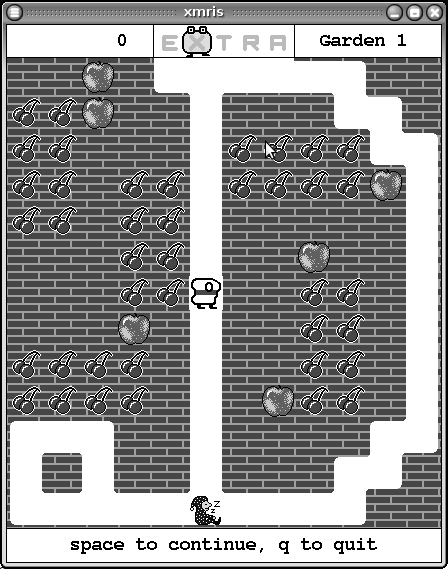
\includegraphics[height=0.5\hsize] {image2011-natsu/xmris-top_mono.png}
 \caption{Xmirsの画面}
\label{fig:xmris-top}
\end{center}
\end{figure}

 で、昔を懐しんでこのXmrisがやりたくなり、早速aptitude search xmrisしてみたところ、

 \begin{center}
  \Large{ごはっ、Xmrisがどこにも無いっ!?}
 \end{center}

 でした。で、「もしや?」と思い、方々捜し回ったところ、
Debian WikiのGames/Suggestedのページ
(\url{http://wiki.debian.org/Games/Suggested})のパッケージにして欲しいリストにXmirsの名前が燦然と輝いているではありませんか。


\subsection{Debian Games Teamへ}

 Xmrisがとにかくやりたかった為、完璧にパッケージ作成初心者ではありましたが、Debian Policy文章、apt-get sourceコマンド、lintianコマンドのお陰で苦労なくパッケージを作成できました。

 が、パッケージは作ったものの、当時、自分の周りにはDDは全くおらず、「どうやったらパッケージを取り込んでもらえるのだろう?」と言う事で悩みまくることになりました。で、辿り着いたのがDebian Game Teamでした。

 右も左も分からない状況で Debian Games TeamのML(\url{debian-devel-games@lists.debian.org}以下ML)でおそるおそるやり取りしたところ以下の事がわかりました。

 \begin{description}
 \item [参加資格]\mbox{}\\
   実際にGameのパッケージをつくろうとしている人はだれでも(初心者ならなおさら入って他の人のパッケージの作り方とやりとりを見てくれと言われた)
 \item [参加方法]\mbox{}\\
   こんな感じで進めます。
   \begin{description}
   \item [Step 1.]まずMLに参加したい意志表明を流す(例:これこれのパッケージを作りたいので入れて欲しい等)
   \item [Step 2.]次にalioth.debian.org(以下alioth)にアカウントを作り(\url{http://alioth.debian.org/account/register.php})、alioth上のDebian Games Teamのページ(\url{http://alioth.debian.org/projects/pkg-games/})にある``Request to join''のリンクから参加のリクエストを送る。
  \item [Step 3.] 後日Debian Games Teamの管理者からWellcomeレターが届き、alioth上のDebian Games TeamのページのProject Membersの欄に名前が登録される。
   \end{description}
 \item [実際の開発]\mbox{}\\
   マニュアル(\url{http://wiki.debian.org/Games/VCS},\url{http://wiki.debian.org/Games/VCS/git})を見てVCS/ML/IRCを活用しながらパッケージ開発を進めることになります。(IRCは、irc.debian.orgサーバー上の\#debian-gamesチャンネル)
   \begin{description}
   \item [Step 1.] マニュアルに従い作ろうとしているパッケージのリポジトリを堀る。(勝手にバンバン掘って良いとの事です)
   \item [Step 2.] gitコマンドを使ってどんどんパッケージの修正をアップロードしていく。
   \item [Step 3.] パッケージが完成したら、mentor.debian.netにアップロードして、mentorを募る。うまくmentorがつけば、Debianのパッケージリリースのプロセスにのるハズ。
   \end{description}
 \end{description}

\subsection{私見}

 以下にDebian Game Teamに関する私見をば。

 \begin{itemize}
 \item ゲームをdebianパッケージにしたい人が情報交換をする為に単に集まる寄合い場所のような位置づけなので、Debian Game Teamとして、ゲームのパッケージを作成する以外の明確なビジョンとかルールがあるわけではない。その為、 Debian Game Teamのエリアに自分のgitリポジトリを掘るときに「こうしていいか?ああしていいか?」といちいち許可を求めると、ウザがられるのは驚いた(最後はあなたの好きにしてくれ、本当にまずかったら指摘を受けるからその時に覚えてくれといわれてしまった。まあ、聞き方の問題だったのかもしれない...)
   \item きっとDebian Game Teamの関係者と面識が在るといろいろやりやすいと思う。
   \item Debian Game Team以外でも身の回りに相談できるDDがいると大変違う(Debianで常識、Debian Game Teamで常識をうまく切り分けられる)
   \item 規模大き目のゲームをパッケージにまとめる際、付属しているバイナリデータ群に
        別のライセンスが適用/良くわからないライセンスが適用されていることがあり、
         こちらの扱いで頭を抱える事がある。
        (キャラクタの画像、背景の画像、ゲーム内部で使われているフォント、サウンドetc...)
   \item 手のかかる問題の解決/ちょっと揉めるリスクのある問題の解決(ライセンス問題、以前のパッケージメンテナ/アップストリームに結局連絡取れない、uploadに関してスポンサーがつかない等)については、消極的。結局、こちらはパッケージメンテしようとする側にて解決が求められる。
   \item MLに流れるやりとりよりも、IRCでのやり取りの方が多い印象。また、話も早い事が多い。MLで回答が得られなくてもがっかりせず、その場合はIRCへ突撃をお勧め。
   \item 空気を読むとpackageを作成する方法、debian policyなどは基礎知識としてある事が前提。
   \item チームに所属している人の生活があふれるやり取りがIRCで日常的に行われているのは新鮮だった。例:今、「会社でたよー。ちょっとまってねー」→ 「はい家についたから繋いだよー。〜の件はねー」と会話が続く。日常生活の一部として、Contribution活動が組み込まれてしまっているのは自分にとっては感動ものでした。
 \end{itemize}

%-------------------------------------------------------------------------------
\dancersection{KinectをDebianで使ってみた}{山田 泰資}
%-------------------------------------------------------------------------------

\index{kinect}
\subsection{Kinectって何?}

KinectはMicrosoftが2010/11にXBox360の新しい操作デバイスとして発売した
ゲームデバイスで、強力な画像認識機能を持ち、一切コントローラなどを
手にしないゲームプレイを実現します。

ハードウェアとしての最大の特徴は、画像認識と言っても単なるカメラではなく、
深度センサを搭載していることです。この種の深度センサ付カメラは従来も
あったのですが、Kinectは大量生産されることもあって価格が1万4千円前後と
従来と比べてまさに桁違いの安さで、このためPCなどの周辺機器として
流用できないかと発売前から高い注目を集めました。

\subsection{発売、そしてKinectハックへ}

そして発売されると普通にUSB接続ができることが判明(単品販売品のみ。
XBox360同梱版はケーブルを加工する必要あり)し、すかさず画像・深度
データのキャプチャ方法が解析されます。こうしてまず生まれたのが
libfreenectです。libfreenectは急速に開発が進み、
\begin{enumerate}
\item カメラ(通常、深度、赤外線)画像の取得
\item カメラのチルト制御
\item 加速度センサの読み出し
\item 筐体LEDの制御
\end{enumerate}
とサウンド関係以外はほぼ制御できるようになり、各種言語へのラッパーが
作られたりOpenCVなどの既成の画像認識ライブラリと組み合わせてデモが
作成されるなど、あっというまに普及が進みました。ここまでが発売後
1ヶ月程の話になります。

しかし、libfreenectだけでは限界がありました。XBox360ではkinectを
使ったゼスチャ認識などの高度な機能を持ったアプリケーション(ゲーム)を
作成できる環境が用意されているのですが、libfreenectはあくまで
ハードウェアにアクセスするまでなので、その部分が欠けていたのです。

実は前評判では「本体側の負荷を下げるため、Kinect側でジェスチャ認識などの
高水準認識も分担する能力がある」という話もあったのですが、最終的には
深度センサまでがハードウェアで、残りはXBox360向けのソフトウェア
ライブラリで実現する形となっていたのでした。

しかし、ここで新展開が起こります。Kinectの深度センサと上記ライブラリの
原型提供を行ったPrimeSense社から、
\begin{enumerate}
\item Linux, Windows用のKinect搭載センサ用ドライバをOSSとして公開する
\item ゼスチャ認識機能を備えた OpenNI フレームワークをOSSとして公開する
\item 骨格認識および高度なジェスチャ認識を行う NITE ライブラリを無償提供する
\footnote{OSSではなく、無償利用のためのライセンスコードが公開された}
\end{enumerate}
という発表が行われ、純正のXBox360開発環境と遜色がなくなり、人気が
さらに高まりました。

これを生かして年末にかけては3Dモデリングツール(MikuMikuDance)に
モーションキャプチャエンジンとして組み込んだり、年明けにはARウルトラ
セブン(画面中の自分の姿にウルトラセブンのコスプレをオーバレイし、
ジェスチャにあわせて様々な必殺技を繰り出すことができる)が登場するなど、
日本では現在進行形で爆発的な盛り上がりを見せています。

ここではOpenNIおよびNITEの利用方法を紹介しつつ、それを元に
Debian勉強会のプレゼンテーションをジェスチャで行う支援ツールの
作成までを紹介します。

\subsection{OpenNIとNITEの導入}
まずはインストールです。
\begin{enumerate}
\item 独自に拡張が始まっているOpenNIとドライバ(SensorKinect)はgithubから
\item NITEはバイナリのためPrimeSense社サイト(\url{http://www.openni.org/})から
\end{enumerate}
それぞれ入手します。

現段階ではバージョンの組み合わせによっては動作しないことがあり、
ここでは以下の組み合わせで導入します:
\begin{enumerate}
\item OpenNI (stable) / \url{https://github.com/OpenNI/OpenNI.git}
\item SensorKinect (avin2 version) / \url{https://github.com/avin2/SensorKinect.git}
\item NITE-Bin-Ubuntu-x64-1.3.0.17.tar.bz2
\end{enumerate}

いくつかのパッケージを入れるなどビルド環境を整えておく必要は
あります
\footnote{apt-get install gcc python2.6 libusb-1.0-0-dev freeglut3-dev doxygen graphviz あたりで整うかと思います}
が、後は付属のドキュメントの通りに進めればトラブルなく導入できました。

まずはOpenNI本体をインストールします:
\begin{commandline}
$ git-clone https://github.com/OpenNI/OpenNI.git
$ cd OpenNI/Platform/Linux-x86/CreateRedist
$ ./RedistMaker # ビルドおよびインストール用バイナリセットを作ります
...
$ cd ../Redist
$ pwd
/d/src/openni/OpenNI/Platform/Linux-x86/Redist
$ sudo ./install.sh
copying shared libraries...OK
copying executables...OK
copying include files...OK
creating database directory...OK
registering module 'libnimMockNodes.so'...OK
registering module 'libnimCodecs.so'...OK
registering module 'libnimRecorder.so'...OK

*** DONE ***
$
\end{commandline}

次にドライバ(といっても、Linux版のものは単なる共有ライブラリです):
\begin{commandline}
$ git-clone https://github.com/avin2/SensorKinect.git
$ cd SensorKinect/Platform/Linux-x86/CreateRedist
$ ./RedistMaker # ビルドおよびインストール用バイナリセットを作ります
...
$ cd ../Redist
$ pwd
/d/src/openni/SensorKinect/Platform/Linux-x86/Redist
$ sudo ./install.sh
creating config dir /usr/etc/primesense...OK
copying shared libraries...OK
copying executables...OK
registering module 'libXnDeviceSensorV2.so' with OpenNI...OK
registering module 'libXnDeviceFile.so' with OpenNI...OK
copying server config file...OK
setting uid of server...OK
creating server logs dir...OK
installing usb rules...OK

*** DONE ***
$
\end{commandline}

そして最後にNITEのインストールです:
\begin{commandline}
$ tar xf NITE-Bin-Ubuntu-x86-1.3.0.17.tar.bz2 -C /d/src/openni/
$ cd Nite-1.3.0.17
$ sudo ./install.bash -l=0KOIk2JeIBYClPWVnMoRKn5cdY4=
...バイナリを/usr/lib等にコピーした後、サンプルコードをビルドする...
$
\end{commandline}

最後のNITEの導入で指定した「0KOIk2JeIBYClPWVnMoRKn5cdY4=」が
無料利用のための公開ライセンスキーになります。

これらのインストールが終わると
\begin{enumerate}
\item /usr/libにlibnim*.so, libXn*.so, libXnV*.so
\item /usr/include/{ni,nite}に各種ヘッダファイル
\item /usr/binにniReg, niLicenseコマンド(モジュールやライセンスの管理用)
\item /var/lib/niにモジュールやライセンスの管理用XMLファイル
\item /usr/etc/primesenseにOpenNIやモジュールの設定・データファイル
\end{enumerate}
という構成になります。/usr/etc/primesenseはLFS的におかしな位置のため、
/var/lib/ni/modules.xmlから参照しているパス設定を変更の上、/etcに
移動させるとよいかもしれません。
\footnote{OpenNIのパッケージを作成予定ですが、このあたりは検証後直す予定}

あと、サンプルコードを動かせるよう一部ファイルを修正しておきましょう。
NITEを展開した Nite-1.3.0.17/Data/ 下のXMLファイルを以下の内容にします。
ライセンスキーの書き込みと、キャプチャ設定の修正・追加になります。

Sample-Scene.xmlの内容:
\begin{commandline}
<OpenNI>
  <Licenses>
    <License vendor="PrimeSense" key="0KOIk2JeIBYClPWVnMoRKn5cdY4="/>
  </Licenses>
  <Log writeToConsole="true" writeToFile="false">
    <!-- 0 - Verbose, 1 - Info, 2 - Warning, 3 - Error (default) -->
    <LogLevel value="3"/>
    <Masks>
    <Mask name="ALL" on="false"/>
    </Masks>
    <Dumps>
    </Dumps>
  </Log>
  <ProductionNodes>
    <Node type="Depth">
      <Configuration>
        <MapOutputMode xRes="640" yRes="480" FPS="30"/>
        <Mirror on="true"/>
      </Configuration>
    </Node>
    <Node type="Scene" />
  </ProductionNodes>
</OpenNI>
\end{commandline}

Sample-Tracking.xmlの内容:
\begin{commandline}
<OpenNI>
  <Licenses>
    <License vendor="PrimeSense" key="0KOIk2JeIBYClPWVnMoRKn5cdY4="/>
  </Licenses>
  <Log writeToConsole="false" writeToFile="false">
    <!-- 0 - Verbose, 1 - Info, 2 - Warning, 3 - Error (default) -->
    <LogLevel value="3"/>
    <Masks>
    <Mask name="ALL" on="true"/>
    </Masks>
    <Dumps>
    </Dumps>
  </Log>
  <ProductionNodes>
    <Node type="Depth" name="Depth1">
      <Configuration>
      <MapOutputMode xRes="640" yRes="480" FPS="30"/>
      <Mirror on="true"/>
      </Configuration>
    </Node>
    <Node type="Gesture" />
    <Node type="Hands" />
  </ProductionNodes>
</OpenNI>
\end{commandline}

Sample-User.xmlの内容:
\begin{commandline}
<OpenNI>
  <Licenses>
    <License vendor="PrimeSense" key="0KOIk2JeIBYClPWVnMoRKn5cdY4="/>
  </Licenses>
  <Log writeToConsole="true" writeToFile="false">
    <!-- 0 - Verbose, 1 - Info, 2 - Warning, 3 - Error (default) -->
    <LogLevel value="3"/>
    <Masks>
    <Mask name="ALL" on="false"/>
    </Masks>
    <Dumps>
    </Dumps>
  </Log>
  <ProductionNodes>
    <Node type="Depth" name="Depth1">
      <Configuration>
      <MapOutputMode xRes="640" yRes="480" FPS="30"/>
      <Mirror on="true"/>
      </Configuration>
    </Node>
    <Node type="User" />
  </ProductionNodes>
</OpenNI>
\end{commandline}

これらの内容の意味については次項で解説します。

\subsection{Kinectを叩いてみる - OpenNIを使ってみよう}
それではOpenNIから使ってみましょう。
以下はサンプルを少しいじって、深度カメラを叩いて深度情報を
取得し、それをPPM画像の形でダンプするようにしてみたものです。

\begin{commandline}
/*BINFMTCXX: -Wall -I/usr/include/ni -I/usr/include/nite -lOpenNI
 *
 * 深度情報のキャプチャを行い、PGM画像として保存する。
 * カメラからの距離がピクセルの濃淡で表される画像になる。
 *
 */

#include <XnCppWrapper.h>

#define log(...) do { \
        fprintf(stderr, __VA_ARGS__); fprintf(stderr, "\n");    \
    } while (0)

#define die(...) do { \
        fprintf(stderr, __VA_ARGS__); fprintf(stderr, "\n"); exit(1);   \
    } while (0)

// 深度センサが返すデータは深度が16bit値で左上から並んでいるので、
// そのまま16bit PGMとしてダンプすれば画像になる。
void
ppmsave(xn::DepthMetaData& meta, const char *outfile) {
    const XnDepthPixel* pix = meta.Data();

    XnUInt32 xmax = meta.XRes();
    XnUInt32 ymax = meta.YRes();

    // dump 16bit depth data as 16bit PGM
    FILE* out = fopen(outfile, "w+");
    fprintf(out, "P5\n%d %d 65535\n", xmax, ymax);
    fwrite(pix, sizeof(XnDepthPixel), xmax * ymax, out);
    fclose(out);
}

int
main(int argc, char **argv) {
    xn::Context context;
    xn::EnumerationErrors errors;
    xn::DepthGenerator dgen;
    xn::DepthMetaData meta;

    if (argc < 3) {
        die("Usage: %s kinect.xml depth.pgm", argv[0]);
    }

    // XML構成ファイルでの初期化、深度カメラへの参照取得、そしてキャプチャ
    context.InitFromXmlFile(argv[1], &errors);
    context.FindExistingNode(XN_NODE_TYPE_DEPTH, dgen);
    context.WaitOneUpdateAll(dgen);

    // キャプチャデータの取得と保存
    dgen.GetMetaData(meta);
    ppmsave(meta, argv[2]);

    context.Shutdown();
    return 0;
}
\end{commandline}

これを実行すると、\footnote{binfmtc パッケージをインストールしておくと、
実行権限をつけておいたC++プログラムを直接シェルから実行するとコンパイル・
実行してくれるようになります。}
\begin{commandline}
$ ./camera3d.cc kinect.xml depth.pgm
\end{commandline}
次のように各ピクセルの深さが画像として取れます:
\begin{center}

\includegraphics[height=6cm]{image201101/depth.eps}
\end{center}
正直何がなんだか?という画像ですが、右側にいるのがノートPCを
膝において座っている私です。

ここでの中核部分は以下の3行です。
\begin{commandline}
context.InitFromXmlFile(argv[1], &errors);
context.FindExistingNode(XN_NODE_TYPE_DEPTH, dgen);
context.WaitOneUpdateAll(dgen);
\end{commandline}

OpenNIではシステム中にどのようなデバイスが存在するか、また、
それらの構成(カメラなら解像度など)はどうなるかを外部のXMLで
記述でき、それを元に初期化を行います。コードだけでも書くことは
できるのですが、その場合は構成を変更するとコードの書き換えが
必要になります。

このコンテキスト(context)を作成し、そこにデバイスやフィルタ(未登場
ですが、センサデータの入力を受けてゼスチャ認識を行い、登録されている
フックをトリガするものなどがあります)といったOpenNIモジュール群を
接続する、というのがOpenNI/NITEのプログラムフローになります。

最後に、上で利用したkinect.xmlも引用しておきます:
\begin{commandline}
<OpenNI>
  <!-- ログ設定。以下の設定で標準出力は使わず Log/*.log に書く -->
  <Log writeToConsole="false" writeToFile="true">
    <LogLevel value="0"/>
    <Masks>
      <Mask name="ALL" on="true"/>
    </Masks>
    <Dumps />
  </Log>

  <ProductionNodes>
    <Node type="Image" name="Kin2D">
      <Configuration>
        <MapOutputMode xRes="640" yRes="480" FPS="30"/>
        <Mirror on="true"/>
      </Configuration>
    </Node>

    <Node type="Depth" name="Kin3D">
      <Configuration>
        <MapOutputMode xRes="640" yRes="480" FPS="30"/>
        <Mirror on="true"/>
      </Configuration>
    </Node>

    <Node type="Scene" />
    <Node type="User" />
    <Node type="Gesture" />
    <Node type="Hands" />
  </ProductionNodes>
</OpenNI>
\end{commandline}
以後の例もすべてこのXMLを使って動かしています。

\subsection{ジェスチャの検出方法 - NITEを使う}
それでは次はジェスチャの認識をさせてみましょう。
こちらではNITEライブラリを利用します。

これもOpenNIフレームワーク上のプログラミングなのでコンテキストを
生成する点は同じですが、NITEではコンテキストを介した深度センサ
データのやりとりのような低レベルの操作は隠され、
\begin{enumerate}
\item ジェスチャー操作の流れを管理する、コンテキストをラップするセッションマネージャ
\item セッションマネージャに登録される各種のジェスチャー検出器
\item それら検出器に登録される、操作検知時に呼び出されるコールバック
\end{enumerate}
という構造のコードになります。操作中・操作終了をセッションマネージャが
判定し、「セッション中」の動作のみが検出器にかかるよう調整しています。

実際にどのようなものになるか、見てみましょう:
\begin{commandline}
/*BINFMTCXX: -Wall -I/usr/include/ni -I/usr/include/nite -lXnVNite -lOpenNI
 *
 * 簡単なジェスチャ認識のテスト。
 * 手を振ってセッション開始すると、プッシュとスワイプ動作を認識する。
 *
 */

#include <XnCppWrapper.h>
#include <XnVNite.h>

/**********************************************************************
 * Utility Functions
 **********************************************************************/

#define log(...) do {                       \
        fprintf(stderr, __VA_ARGS__);       \
        fprintf(stderr, "\n");              \
    } while (0)

#define die(...) do {                       \
        fprintf(stderr, __VA_ARGS__);       \
        fprintf(stderr, "\n");              \
        exit(1);                            \
    } while (0)

/**********************************************************************
 * セッションマネージャや検出器に登録するコールバック関数
 * 現在は個々のジェスチャーを認識した等のログを出すのみ。
 **********************************************************************/

static void
OnSessionStart(const XnPoint3D &p, void *data) {
    log("session start");
}

static void
OnSessionEnd(void *data) {
    log("session end");
}

static void
OnFocusStartDetected(const XnChar *focus,
                     const XnPoint3D &p, XnFloat progress, void *data) {
    log("focus start");
}

static void
OnSwipe(XnVDirection dir, XnFloat speed, XnFloat angle, void *data) {
    log("swipe detected. dir=%d, speed=%f, angle=%f", dir, speed, angle);
}

static void
OnPush(XnFloat speed, XnFloat angle, void *data) {
    log("push detected. speed=%f, angle=%f", speed, angle);
}

/**********************************************************************
 * Main
 **********************************************************************/

int
main(int argc, char **argv) {
    xn::Context context;

    if (argc < 2) {
        die("Usage: %s kinect.xml", argv[0]);
    }

    context.InitFromXmlFile(argv[1]);

    // セッションマネージャと各種検出器の生成
    XnVSessionManager* sm = new XnVSessionManager;
    XnVSwipeDetector*  sd = new XnVSwipeDetector;
    XnVPushDetector*   pd = new XnVPushDetector;

    // セッションマネージャの初期化
    //
    // 手を振って(Wave)セッションに入り、休止状態からのセッション再開は
    // 手を上げる(RaiseHand)。セッション中は下で登録された検出器が操作を
    // 検出するようユーザの動きをそれらに伝達する。
    sm->Initialize(&context, "Wave", "RaiseHand");
    sm->RegisterSession(NULL,
                        OnSessionStart, OnSessionEnd, OnFocusStartDetected);

    // ジェスチャー検出器と検知した際のコールバックを登録
    sm->AddListener(sd);
    sm->AddListener(pd);
    sd->RegisterSwipe(NULL, OnSwipe);
    pd->RegisterPush(NULL, OnPush);

    // 後はずっと入力を待ってはイベント処理するループ
    context.StartGeneratingAll();
    for (;;) {
        context.WaitAndUpdateAll();
        sm->Update(&context);
    }
    return 0;
}
\end{commandline}

最初の深度データの画像を保存する例よりも簡単になりました。
上では XnVSwipeDetector と XnVPushDetector の2種類だけを使いましたが、
NITEには10を超える様々な基本ジェスチャーの検出器があり、また、
複数のジェスチャーを組み合わせた操作に対応するための複合処理などを
行う補助クラスも用意されています。

このように、多種多様な検出器を用意して、煩雑な体の各部の動きの
トラッキングや照合の手間をNITEは省いてくれます。

\begin{itembox}[l]{各種の操作と認識率}
なお、動かしてみるとわかりますが、動作によって「きちんと認識される」度が
結構違います。スワイプは「一瞬手を止めて、それからさっと流す」動作なのですが
非常に認識率が悪いです。一方、プッシュ操作はほぼ確実に認識されます。
プッシュ(Push, Click)動作は手振り(Wave)動作と並んで「セッション開始の
シグナル動作(focus gesture)」として実用的とマニュアルに書かれていますが、
よくわかります。快適な操作感のためには結局カスタムの検出器を作成する必要が
ありそうです。
\end{itembox}

\subsection{アプリケーションの制御方法 - XTestの話}
さて、これまでOpenNI, NITEと例を出してきましたが、次はこれで
認識したジェスチャでどう他のアプリケーションを制御するかです。
今回はX11のxtst(XTest)拡張でマウスやキーイベントを送り、それで
(この資料の)プレゼンテーションが行えるようにします。

XTest自体の使い方は以下のようになります。
\begin{commandline}
/*BINFMTCXX:-Wall -lXtst -lX11
 * XTestを使ったキーとマウスの制御テスト
 */

#include <stdio.h>
#include <stdlib.h>
#include <unistd.h>

#include <X11/Xlib.h>
#include <X11/Xutil.h>
#include <X11/extensions/XTest.h>

#define log(...) fprintf(stderr, __VA_ARGS__)
#define die(...) do { fprintf(stderr, __VA_ARGS__); exit(1); } while (0)

enum { DOWN = 1, UP, DOWNUP };

void
sendkey(Display *disp, unsigned int keysym, int mask) {
    unsigned int kc = XKeysymToKeycode(disp, keysym);
    if (mask & DOWN) { XTestFakeKeyEvent(disp, kc, True, CurrentTime); }
    if (mask & UP)   { XTestFakeKeyEvent(disp, kc, False, CurrentTime); }
    XSync(disp, False);
}
int
main(int argc, char **argv) {
    Display *disp;

    if ((disp = XOpenDisplay(NULL)) == NULL) {
        die("Unable to open display\n");
    }

    // キー入力のテスト - とりあえず ls させてみる
    unsigned int key[] = { XK_L, XK_S, XK_Return };
    for (int i = 0; i < (int)(sizeof(key) / sizeof(*key)); i++) {
        sendkey(disp, key[i], DOWNUP);
    }

    // 相対位置移動
    XTestFakeRelativeMotionEvent(disp, -100, -100, CurrentTime);
    XSync(disp, False);
    sleep(3);

    // 絶対位置移動
    XTestFakeMotionEvent(disp, -1, 100, 100, CurrentTime);
    XSync(disp, False);
    sleep(3);

\end{commandline}
\begin{commandline}
    // XTestのFakeMotionでなぜかXMing上のポインターが動かないので、
    // XWarpPointerを使ってみるテスト・・・これだと動くようだ。
    XWarpPointer(disp, None, None, 0, 0, 0, 0, 200, 200);
    XSync(disp, False);
    sleep(3);

    // Control押しながら右クリックを実行(メニューが出るか確認)
    sendkey(disp, XK_Control_L, DOWN);
    XTestFakeButtonEvent(disp, 3, True,  CurrentTime);
    XTestFakeButtonEvent(disp, 3, False, CurrentTime);
    sendkey(disp, XK_Control_L, UP);
    XSync(disp, False);

    // 終了
    XTestDiscard(disp);
    XCloseDisplay(disp);

    return 0;
}
\end{commandline}

操作したいアプリケーションに合わせて
\begin{enumerate}
\item XTestFakeKeyEvent
\item XTestFakeButtonEvent
\item XTestFakeMotionEvent
\item XTestFakeRelativeMotionEvent
\end{enumerate}
で操作イベントを送りながら、XSyncで同期を取る(ポインタを移動させて
入力、のような操作で、移動が完了してから入力がされるようにする)というのが
基本的な処理になります。

あとはこれを先のOpenNI/NITEのジェスチャ検知をトリガに発行してやれば、
今回のデモは完成になります。

\subsection{デモ}
さて当日うまくいくか・・・(当日の結果:いくらKinectの前で踊っても
反応が鈍すぎで、スライドを3枚めくった所で聴衆からお役御免を言い渡されたの
だった・・・。NUI難しい)

%-------------------------------------------------------------------------------
\dancersection{俺のlibsaneが火を噴くぜ!}{本庄 弘典}
%-------------------------------------------------------------------------------
\index{libsane}

SANEはScanner Access Now Easyの頭文字を取ったもので、各種デバイスから画
像を取り出すための汎用インターフェースです。主にスキャナから画像を取得
するため、LinuxやFreeBSDなどフリーなOSで利用されます。

今回はSANEの仕組みとlibsaneを用いたプログラムの作成方法について解説します。

\subsection{SANEの構造}

SANEを利用するアプリケーションはlibsane.soという共有ライブラリをリンク
します。libsane.soはdllと呼ばれる仮想デバイスドライバを通し、各デバイス
ごとに作られたドライバにアクセスすることでデバイスを制御します。また図
に示されるように、net仮想ドライバで他のマシンのsanedに接続することで、
リモートスキャナへのアクセスを実現します。
\cite{sane,sanejp,saneapi}

\begin{figure}[H]
\begin{center}
 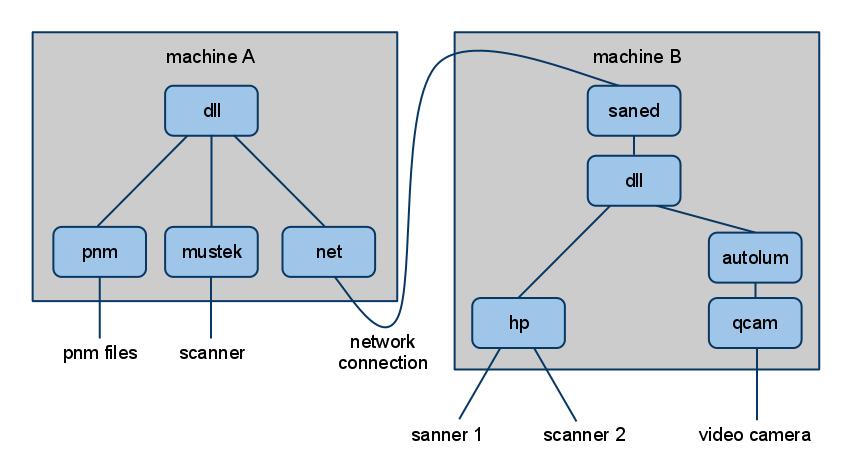
\includegraphics[height=0.5\hsize] {image201012/libsane02.png}
 \caption{SANEの構造}
\label{fig:sane}
\end{center}
\end{figure}

なお、
SANEを利用するユーザはscannerグループに所属させる必要があります。

\subsection{Code Flow}

\begin{figure}[H]
\begin{center}
 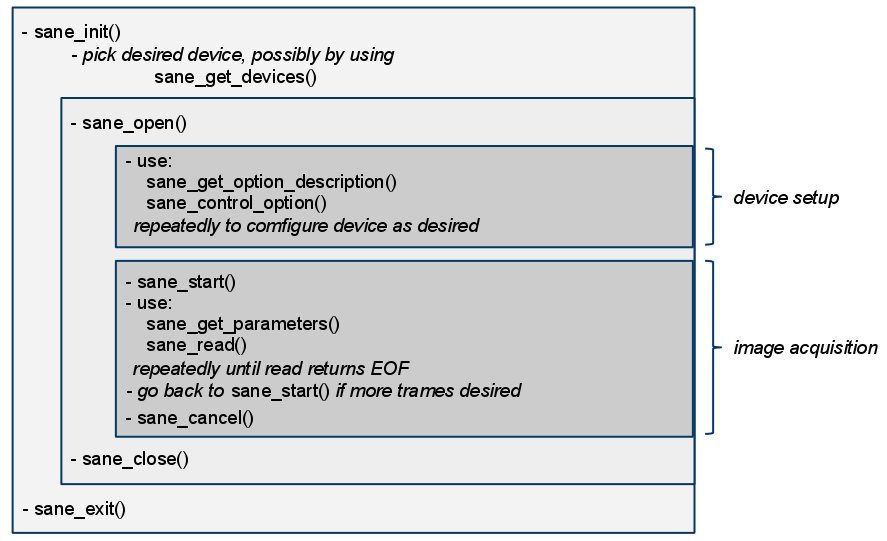
\includegraphics[height=0.5\hsize] {image201012/codeflow.png}
 \caption{Code Flow}
\label{fig:codeflow}
\end{center}
\end{figure}


\subsection{スキャンするためのコード}

とりあえずスキャンするだけのコードは次のようになります。

\begin{commandline}
#include <stdio.h>
#include <stdlib.h>
#include <string.h>

#include <sane/sane.h>


#define MAXLEN 32768

int main()
{
  SANE_Status stat;
  SANE_Handle hndl;
  SANE_Byte buf[MAXLEN];
  SANE_Int len = MAXLEN;
  FILE *fp;

  stat = sane_init(NULL, NULL);
  printf("init: %d\n", stat);
  stat = sane_open("fujitsu:libusb:008:002", &hndl);
  printf("open: %d\n", stat);

  fp = fopen("foo.bin", "wb");
  stat = sane_start(hndl);
  printf("start: %d\n", stat);
  while (len == MAXLEN) {
    stat = sane_read(hndl, buf, MAXLEN, &len);
    printf("read: %d\n", stat);
    printf("read_len: %d\n", len);
    fwrite(buf, len, 1, fp);
  }
  fclose(fp);

  sane_close(hndl);
  printf("close: %d\n", stat);
  sane_exit();
  printf("exit: %d\n", stat);
}
\end{commandline}

このコードで保存されるfoo.binは、
ScanSnap S1500の場合、
ヘッダ無しのpbmファイルとして保存されました。
スキャナによってはpgmで保存されるものもあり、
デフォルトで保存される画像のモードは特に決まっていないようです。


\subsection{カラーのスキャン}

オプションの設定にはいくつか注意点があるようです。

\begin{itemize}
\item sane\_get\_option\_descriptor()でオプションの説明文やフォーマットの取得が可能。
\item sane\_control\_option(hndl, 0, SANE\_ACTION\_GET\_VALUE, \&num, \&info)でオプションの総数を取得できる。
\item sane\_control\_option()でActionにSANE\_ACTION\_GET\_VALUEを指定することで現在設定されているオプションを読み出すことが可能。
\item sane\_control\_option()でActionにSANE\_ACTION\_SET\_VALUEを指定することでオプションの設定が可能。
\item sane\_control\_option()を呼ぶ際には事前にsane\_get\_option\_descriptor()を呼び出しておく必要がある。
\end{itemize}

\begin{commandline}
#include <stdio.h>
#include <stdlib.h>
#include <string.h>
#include <sane/sane.h>

#define MAXLEN 32768

int main()
{
  SANE_Status stat;
  SANE_Handle hndl;
  const SANE_Option_Descriptor *opt;
  SANE_Int info = 0;
  SANE_Byte buf[MAXLEN];
  SANE_Int len = MAXLEN;
  SANE_Parameters param;
  FILE *fp;

  stat = sane_init(NULL, NULL);
  printf("stat: %d\n", stat);
  stat = sane_open("fujitsu:libusb:008:004", &hndl);
  printf("open: %d\n", stat);

  int x=300, y=300;
  opt = sane_get_option_descriptor(hndl, 4);
  printf("get_option_descriptor: %03d: %d\n", 0, opt->size);
  stat = sane_control_option(hndl, 4, SANE_ACTION_SET_VALUE, &x, &info);
  printf("control_option: %d\n", stat);
  printf("info: %d\n", info);

  opt = sane_get_option_descriptor(hndl, 5);
  printf("get_option_descriptor: %03d: %d\n", 0, opt->size);
  stat = sane_control_option(hndl, 5, SANE_ACTION_SET_VALUE, &y, &info);
  printf("control_option: %d\n", stat);
  printf("info: %d\n", info);

  strcpy(buf, "Color");
  opt = sane_get_option_descriptor(hndl, 3);
  printf("get_option_descriptor: %03d: %d\n", 0, opt->size);
  stat = sane_control_option(hndl, 3, SANE_ACTION_SET_VALUE, buf, &info);
  printf("control_option: %d\n", stat);
  printf("info: %d\n", info);

  stat = sane_start(hndl);
  printf("%d\n", stat);
  fp = fopen("foo.ppm", "wb");

  stat = sane_get_parameters(hndl, &param);
  printf("get_parameters: %d\n", stat);
  sprintf(buf, "P6\x0a# SANE data follows\x0a%d %d\x0a%d\x0a",
    param.pixels_per_line, param.lines, 255);
  fwrite(buf, strlen(buf), 1, fp);


  while (len == MAXLEN) {
    stat = sane_read(hndl, buf, MAXLEN, &len);
    printf("read: %d\n", stat);
    printf("read_len: %d\n", len);
    fwrite(buf, len, 1, fp);
  }
  fclose(fp);

  sane_close(hndl);
  printf("close: %d\n", stat);
  sane_exit();
  printf("exit: %d\n", stat);
}
\end{commandline}


\begin{figure}[H]
\begin{center}
 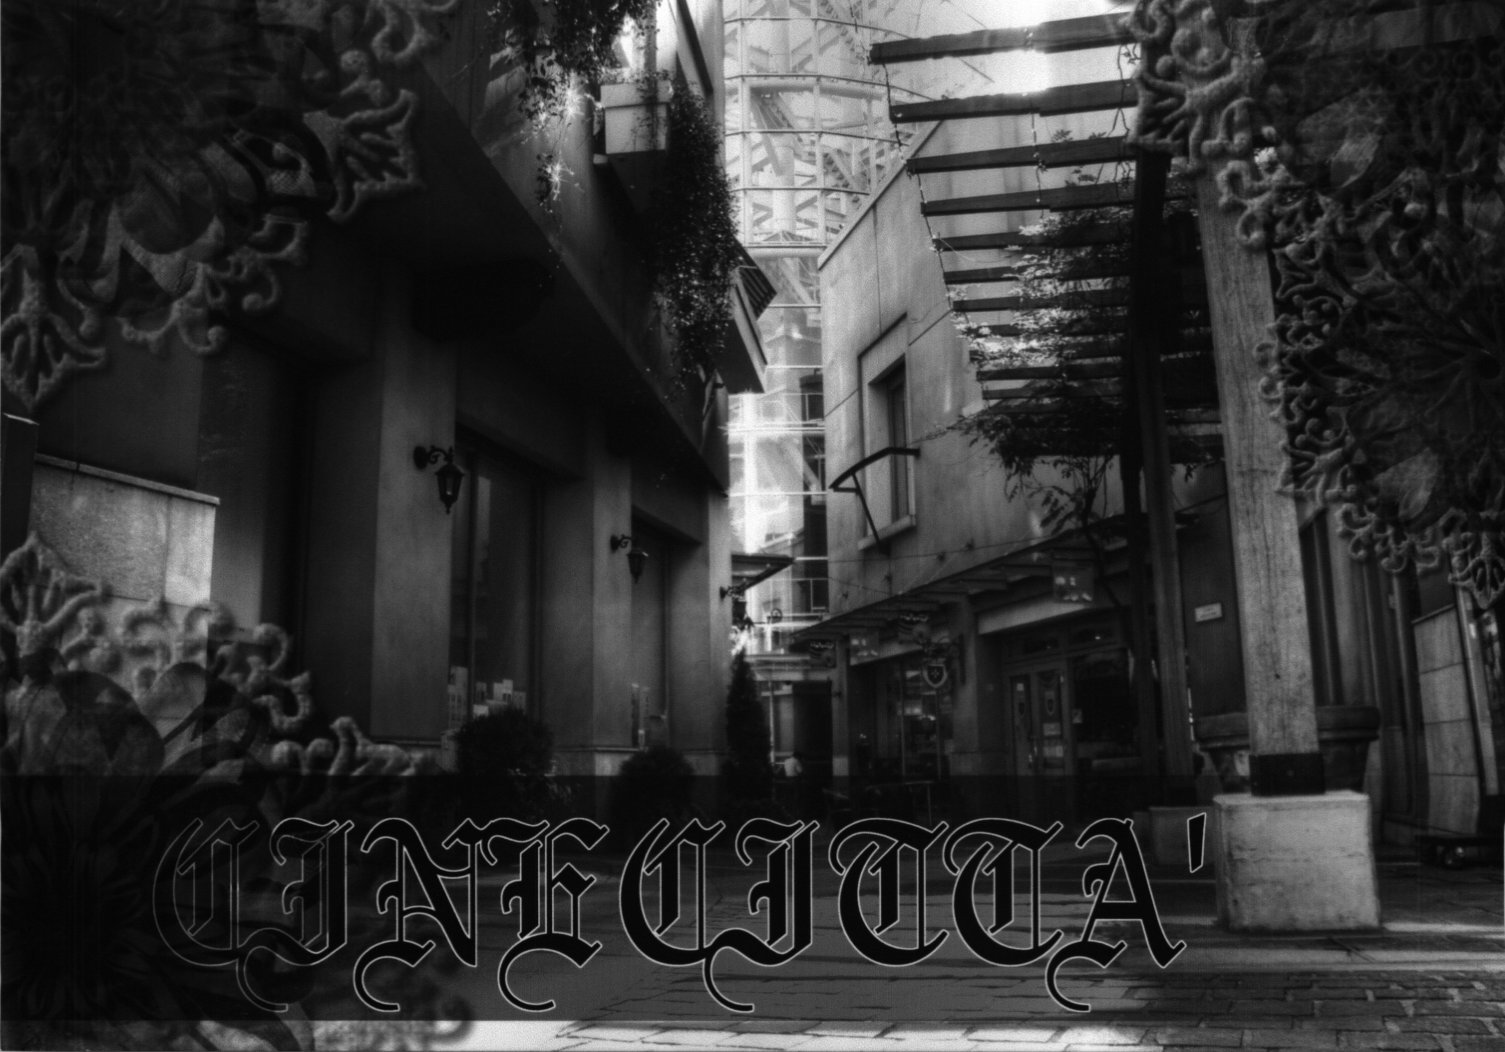
\includegraphics[height=0.5\hsize] {image2011-natsu/dst02_mono.jpg}
 \caption{スキャン結果}
\label{fig:scan}
\end{center}
\end{figure}

モノクロではわかりづらいと思いますが、
ScanSnap S1500でスキャンした結果、
RとBが入れ替わってスキャンされました。

\subsection{まとめ}

\begin{itemize}
\item やや不安定(特に権限周り)
  \begin{itemize}
  \item scanimage -Lでたまにsegmentation faultする
  \end{itemize}
\item スキャナによってデフォルトの動作がまちまち
  \begin{itemize}
  \item ScanSnapは.pbmでスキャン
  \item CanoScanは.pgmでスキャン
  \end{itemize}
\item スキャナによってRGBの順番すらまちまち
  \begin{itemize}
    \item でもこれはScanSnapが悪いのかも
    \item ScanSnapはTWAIN未対応だし
  \end{itemize}
\item ドキュメント化されていない罠の存在
\item スキャナのボタンをイベントとして使えないっぽい
\end{itemize}

\begin{thebibliography}{0}
 \bibitem{sane}SANE - Scanner Access Now Easy \\
\url{http://www.sane-project.org/}

 \bibitem{sanejp}
SANE-tutorial-JP / 著者:David Mosberger / 翻訳:川岸 良治\\
\url{http://archive.linux.or.jp/JF/JFdocs/SANE-tutorial-JP.html}

 \bibitem{saneapi}
SANE Standard Version 2.0 proposal 0.08 - rauch/beck \\
\url{http://www.sane-project.org/sane2/0.08/}

\end{thebibliography}

%-------------------------------------------------------------------------------
\dancersection{Proxmox VE の紹介}{森山 京平}
%-------------------------------------------------------------------------------
\index{Proxmox VE}

\label{sec:moriyama}
\subsection{自己紹介・経歴・概要}
森山 京平(23)\\
\\
NAIST(奈良の森の中の大学院)\\
Ubuntu User\\
Debianは、サーバ用途でしか触ったことがない。\\
最近は、もっぱら、仮想化技術に興味をもち、KVM を触って自己満足の世界にひ
たっている。某プロジェクト\footnote{AI3 \url{http://www.ai3.net}}のネッ
トワークエンジニア兼サーバエンジニアに任命され、四苦八苦しながらネットワー
ク・サーバの運用と管理を行っている。今年 AI3 Project では、10 年ほど運用
してきたサーバ(物理マシン)のリプレイスを行うようになった。そこで、近年
話題になっている、仮想化技術を用いて、サーバの台数を減らし、可用性を増す
ことを試みた。機器の設置や、dom0(仮想化のベースとなるサーバ)の設定は、
ほぼ終了。仮想マシンで実行するサービスのテストも無事に終わった。今後、次々
に移行していく予定である。KVM を用いて完全仮想化を行うという要求があった
ので、どうしようと迷っていた所、Debian ベースで開発が進んでいる、
ProxmoxVE という OSS に出会い、それを採用させて頂いた。今回は、その
ProxmoxVE について簡単にご説明させていただこうと思う。

\subsection{Proxmoc VEとは}
ProxmoxVEとは、Proxmox Server Solutions GmbH によって開発されている、
Debian ベースでかつ web、cli から仮想マシンを操作できる KVM\&OpenVZ マネー
ジメントツールである。perl と shell を使い qemu や kvm コマンドをうまく
組み合わせて web 上からの操作を可能にしている。競合しているツールとして
同じく web から操作できる KVM のマネージメントツールの karesansui がある。
こちらは国内産であり、100\%PurePython で書かれている。優位性云々は、
karesansui をあまりあたったことがないのでわからない。ProxmoxVE のスター
トは、メールゲートウェイの仮想化を行い、セキュリティを高める目的の仮想化
環境である proxmox という OSS からスタートしている。proxmox から得た知見
を proxmox VEにも適用している。現在の最新バージョンは、1.7 であり、2.0
のリリースが予定されている。ダウンロードは \url{http://www.proxmox.com/}
からできる。

\subsection{インストール}
さて、インストールの方法を説明したい。そのまえに、dom0 マシンに対しての
要求がある。KVM による完全仮想化を実現するために、お持ちのマシンの CPU
が Intel-VT もしくは AMD-V に対応しておかなければならない。もしも、
OpenVZ のみを使うのであれば、それらは、必須ではない。しかしながら、パフォー
マンスとしては、完全仮想化であるほうが、優位であると参考までに覚えておいていただきたい。

\subsubsection{ダウンロード}
ProxmoxVE のイメージをダウンロードする。\url{http://www.proxmox.com/} こ
こから donwnload リンクをたどって行くと iso をダウンロードできる。ダウン
ロードした iso を CD なり DVD に焼く。

\subsubsection{ProxmoVE のインストール}
インストール手順は、至ってシンプル。マシンの性能にもよるが、15 分程度で仮想環境が手に入る。

\subsection{web インターフェースからの各種操作}
ProxmoxVE では、基本的に操作を web インターフェース上から行うように設計
されている。ログイン画面からログインを行うことで、Web 管理コンソールに入ることができる。ログインを終えると、ホストマシンのカレントステータスが表示される。\footnote{CPU、メモリ、カーネルのバージョンなど}

\subsubsection{VM マネージャ}
VM マネージャの欄には、仮想マシン、テンプレート、ISO イメージという項目
が存在する。仮想マシンでは、仮想マシンの状態、作成、マイグレートの操作を
行うことができ、テンプレートでは、OpenVZ のテンプレートに関する操作がで
きる。また、ISO イメージにおいては、OS のインストールディスクのイメージ
をアップロードできる。テンプレートは OpenVZ から、ISOイメージは KVM から用いる。

\paragraph{リスト}
ここから、仮想マシンのそれぞれのメンテナンスタスク、カレントステータスを確認することができる。

\subparagraph{仮想マシンの設定}
実行中の仮想マシンの欄をクリックすることで仮想マシンの設定画面に遷移する。仮想マシンの操作や設定はここから行う。

\begin{itemize}
 \item 仮想マシンの設定[仮想マシンのディスク領域、メモリ、スワップなどの設定]
 \item 仮想マシン削除[仮想マシンの削除をおこなう(復元不可)]
 \item 仮想マシン起動[仮想マシンの起動をおこなう]
 \item 仮想マシン再起動[仮想マシンの強制再起動をおこなう]
 \item 仮想マシンシャットダウン[仮想マシンの強制シャットダウンを行う]
 \item 仮想マシン停止(サスペンド?)[仮想マシンのサスペンドをおこなう(未実装?)]
 \item VNC コンソールへのアクセス[JAVA アプレット-VNC でコンソールへアクセスする]
\end{itemize}

\paragraph{作成}
仮想マシンの作成をおこなう。KVM に対応していれば、KVM の項目が出てくる、
そうでなければ、タイプの欄に OpenVZ の項目しか出てこない。それぞれのパラ
メータの設定おこない、”作成する”をクリックすることで、仮想マシンの作成をおこなえる。

\paragraph{マイグレート}
ProxmoxVEでは、CLI から pveca コマンドを用いることでクラスタリングを行う
ことができる。クラスタリングを行った物理マシン間で仮想マシンのマイグレー
トが可能である。今回は、端折らせていただくが、物理マシンのメンテナンスの
際に役立つ機能である。

仮想マシンの項目から、ほとんどの管理を行うことができる、その点が
ProxmoxVE の素晴らしいとこである。詳細な管理や設定を行いたい場合には、
CLI(ssh によるアクセス)でおこなう。CLI のベースは debian であるので、かなり使いやすい印象をうけた。

\subsubsection{設定}
設定には、システム、ストレージ、バックアップの項目が存在する。

\paragraph{システム}
ネットワーク、DNS、時刻、管理、オプションの項目があり、ネットワークでは、
おもにネットワークインターフェースの設定を行う。DNS では、DNS の設定を行
い、サード DNS サーバまで設定を行える。時刻は、時間帯の設定(JST など)
の設定を行う。NTP サーバの設定ができるかと思ったらそうではなく、もし特定
の NTP サーバの設定を行いたい場合は、CLI からの設定が必要であるように思
う(未確認)。管理の項目からは、管理者の E-mail、パスワードの設定が行え
る。オプションからは、言語とキーボード、HTTP プロキシの設定を行える。

\subparagraph{ストレージ}
ストレージの設定を行う。ストレージの追加削除を行う。iSCSI、NFS、LVMグルー
プ、ディレクトリの参照をおこなうことが可能である。

\subparagraph{バックアップ}
ストレージの項目から、バックアップストレージの指定があれば、ここから、バックアップの設定をおこなうことができる。定期的な仮想マシンのバックアップを行うことができる。

\paragraph{管理}
管理の項目には、サーバ、ログ、クラスタがある。

\subparagraph{サーバ}
サーバのサービスの起動、停止、再起動を行うことができる。SSL証明書もここからダウンロードできる。またサーバそのものの再起動、シャットダウンも行える。

\subparagraph{ログ}
タスクのログ、syslog の確認を行えることは、認識しており、仮想化初心者ユー
ザの敷居を低くする有用な OSS であるかと思う。もし、詳細をしりたい方がい
らっしゃれば、ProxmoxVE の Wiki\cite{proxmoxvewiki}を参照していただけたらと思う。

\begin{thebibliography}{}
 \bibitem{proxmoxvewiki} ProxmoxVE Wiki, \url{http://pve.proxmox.com/wiki/Main_Page}
\end{thebibliography}

%-------------------------------------------------------------------------------
\dancersection{Apache2 のモジュールをつくってみた}{上川 純一}
%-------------------------------------------------------------------------------
\index{apache}

Apache httpd というウェブサーバがあります。おそらく定番と言われるウェブ
サーバで、多くの人が利用していると思います。ウェブサーバとして多くの機能
を提供しているApacheですが、モジュールという仕組みで機能拡張可能です。
今回はDebian上でApacheモジュールを作る方法をさぐってみることにします。

\subsection{Apacheモジュールをつくりたいとき}

Apacheモジュールが作りたいときはどういうときでしょうか。作りたいと思った
ときがつくりどき。cgiでfork する手間が惜しい、インタプリタ言語でインタプ
リタが走っている時間がもったいない、GCのある言語でときどき反応が悪くなる
のが気にくわない。いろんな理由があるとおもいますが、C言語でがりがりとウェ
ブリクエストを処理したいとかそういう要望があるのではないでしょうか。

Apacheモジュールでできることはどういうことでしょうか。Apacheの受け取る入
力(HTTP Request)から出力(HTTP Response)のほぼ任意の場所にフックとして割り
込むことができて、入出力のデータを加工することが可能です。

\subsection{Debian の Apache パッケージの構成}

ところで、httpd と Debian apache2 はどれくらい違うかご存知でしょうか。

Debian パッケージのREADME.Debian を見てみましょう。
\cite{Apache2ReadmeDebian}

ざっと眺めただけでも以下の点で特徴があります。

\begin{itemize}
 \item  apache2コマンドが環境変数に依存している。
 \item  apache2ctl / /etc/init.d/apache2 を利用しないと起動とかできない。
 \item  設定ファイルの配置が全然違う。
 \item  a2enmod / a2dismod コマンドが追加されている。
 \item  apxs コマンドが apxs2 という名前になっている。
\end{itemize}

\subsection{Apacheモジュールの作成}

普通のApacheモジュールの作成の流れをみてみましょう。

\subsubsection{パッケージの準備}

とりあえず開発環境をインストールしましょう。
\begin{commandline}
# apt-get install apache2-threaded-dev
\end{commandline}

\subsubsection{テンプレート生成}

apxs2 コマンドを利用してテンプレートを作成します。
モジュール名でディレクトリが作成されます。
\index{apxs2}

\begin{commandline}
$ apxs2 -g -n dancerqps
$ cd dancerqps
$ ls
Makefile  mod_dancerqps.c  modules.mk
\end{commandline}

\subsubsection{ソースコード編集}

ソースコードを編集しましょう。この場合、自動で生成された
\url{mod_dancerqps.c}がメインのモジュールソースコードです。

まず一番下に一番重要な構造が定義されています。ここで重要なのは
\verb!dancerqps_register_hooks! を登録しているところでしょうか。

\begin{commandline}
module AP_MODULE_DECLARE_DATA dancerqps_module = {
    STANDARD20_MODULE_STUFF,
    NULL,                  /* create per-dir    config structures */
    NULL,                  /* merge  per-dir    config structures */
    NULL,                  /* create per-server config structures */
    NULL,                  /* merge  per-server config structures */
    NULL,                  /* table of config file commands       */
    dancerqps_register_hooks  /* register hooks                      */
};
\end{commandline}


\verb!dancerqps_register_hooks!で実際にフックの登録を行います。
ここでは、アウトプットフィルタを登録しています。
\begin{commandline}
static void dancerqps_register_hooks(apr_pool_t *p) {
  ap_register_output_filter(dancerqps_name, dancerqps_filter,
			    NULL, AP_FTYPE_RESOURCE);
}
\end{commandline}

そして、実際に各リクエストのアウトプットに対して実効するフィルタのコード
を書きます。

\begin{commandline}
static apr_status_t dancerqps_filter(ap_filter_t *f, apr_bucket_brigade *bb) {
  /* ここでなにか処理をする */
  ap_log_rerror(APLOG_MARK, APLOG_ERR, 0, f->r,
		"dancerqps processing was here!");
  return ap_pass_brigade(f->next, bb);
}
\end{commandline}

\subsubsection{モジュールのファイルインストール}

モジュールをビルドしてインストールする一連の手順をしてくれるコマンドがあ
ります。

\begin{commandline}
$ sudo apxs2 -c -i mod_dancerqps.c
\end{commandline}

\subsubsection{モジュールを有効にする}

apxs2 コマンドでモジュールを有効にする方法は Debian独自のa2enmodなどのコマンドの存在
を無視しているようなのでa2enmodなどと整合性のとれるような方法をとるのが
よいでしょう。
で、それではDebian的な方法とはなんでしょうか。

\subsubsubsection{Debian way 1}

めんどくさい方法だけどシステム運用者としては便利かもしれない方法。
a2enmodとかができます。

/etc/apache2/mods-available に hoge.conf, hoge.load ファイルを作成します。
hoge.conf は設定が不要なら不要ですが、httpd.confに書くような内容を記述し
ます。
hoge.load には LoadModule行を記述します。

この方法でファイルを作成しておけば、/etc/apache2/mods-enabledディレクト
リにシンボリックリンクが作成されます。

\subsubsubsection{Debian way 2}

デフォルトでは空のファイルだけど、/etc/apache2/httpd.conf に書き込むとそ
の設定が有効になります。

\begin{commandline}
LoadModule test_module /usr/lib/apache2/modules/mod_test.so
<Location "/hoge/">
   SetHandler test
</Location>
\end{commandline}

\subsubsubsection{Debian的な方法から乖離しているっぽい方法}

apache をコマンドラインから設定ファイルを指定して起動することができます。
DebianのApacheは環境変数を設定しないと直接は起動できなくなっているので、
面倒な手続きが必要になります。

まず、適当にテスト用のhttp.confをでっち上げます。

\begin{commandline}
Listen 8080

LockFile /home/test/tmp/apache.1.lock
PidFile /home/test/tmp/apache.1.pid

# log configuration.
LogFormat "%h %l %u %t \"%r\" %>s %b" common
CustomLog "/home/test/log/access_log" common
ErrorLog "/home/test/log/error_log"

# Order, Allow.
LoadModule authz_host_module /usr/lib/apache2/modules/mod_authz_host.so
# map from / -> /index.html
LoadModule dir_module /usr/lib/apache2/modules/mod_dir.so
DirectoryIndex index.html index.cgi index.pl index.php index.xhtml index.htm
# .html -> content-type: text/html
LoadModule mime_module /usr/lib/apache2/modules/mod_mime.so
TypesConfig /etc/mime.types

# Document root
DocumentRoot "/home/test/hoge"
<Directory "/home/test/hoge">
    Options Indexes FollowSymLinks

    AllowOverride None

    Order allow,deny
    Allow from all

</Directory>

# Load my custom filter.
LoadModule dancerqps_module /usr/lib/apache2/modules/mod_dancerqps.so
SetOutputFilter DANCERQPS
\end{commandline}

適当な設定ファイルを指定してApacheを起動してみます。

\begin{commandline}
APACHE_RUN_USER=dancer \
 APACHE_RUN_GROUP=dancer \
 /usr/sbin/apache2 -f $(readlink -f ./httpd.conf) -k restart
\end{commandline}
% $

\subsubsection{負荷テスト}
\index{ab}

ab (apachebench) ツールが標準で入っているのでそれで計測します。適当に確
認しましょう。

\begin{commandline}
$ /usr/sbin/ab -c 100 -n 100 http://localhost:8080/
This is ApacheBench, Version 2.3 <$Revision: 655654 $>
Copyright 1996 Adam Twiss, Zeus Technology Ltd, http://www.zeustech.net/
Licensed to The Apache Software Foundation, http://www.apache.org/

Benchmarking localhost (be patient).....done


Server Software:        Apache/2.2.9
Server Hostname:        localhost
Server Port:            8080

Document Path:          /
Document Length:        44 bytes

Concurrency Level:      100
Time taken for tests:   0.056 seconds
Complete requests:      100
Failed requests:        0
Write errors:           0
Total transferred:      29600 bytes
HTML transferred:       4400 bytes
Requests per second:    1796.17 [#/sec] (mean)
Time per request:       55.674 [ms] (mean)
Time per request:       0.557 [ms] (mean, across all concurrent requests)
Transfer rate:          519.21 [Kbytes/sec] received

Connection Times (ms)
              min  mean[+/-sd] median   max
Connect:        7    9   0.5      9      10
Processing:     9   26   8.9     27      40
Waiting:        6   26   9.3     27      40
Total:         16   36   8.9     37      49

Percentage of the requests served within a certain time (ms)
  50%     37
  66%     41
  75%     43
  80%     45
  90%     47
  95%     48
  98%     49
  99%     49
 100%     49 (longest request)
\end{commandline}

\subsubsection{まとめ}

はじめてApacheモジュールを作成して、インストールして動かすところまでやっ
てみました。


\begin{thebibliography}{}
 \bibitem{Apache2ReadmeDebian} Debian の Apache2 パッケージの README.Debian ファイ, \url{/usr/share/doc/apache2.2-common/README.Debian.gz}
\end{thebibliography}

%-------------------------------------------------------------------------------
\dancersection{CAcert の準備に何が必要か}{山田 泰資}
%------------------------------------------------------------------------------

\index{CACert}

\subsection{CAcertって何?}
CAcertプロジェクトとは誰もが低コストに証明書を持てるようにすることで、
安全な環境・通信を広く実現しようというプロジェクトです。2002年に発足し、
2003年には非営利法人のCAcert Inc.がオーストラリアで設立され、以来
7万人のメンバーに対して18万件の証明書(クライアント認証用、
サーバ認証用、S/MIME署名用、コード署名用、etc)を発行してきています。

通常、個人や組織内で自己発行した証明書は「オレオレ証明書」などと
呼ばれてあくまで閉じた世界での利用になります。しかし、この
プロジェクトではCAcertがルート証明機関として、そのルート証明書が
各種OSやブラウザに組み込まれ、VeriSign社などによる商用サービスに
近い水準で世界的に信頼される状態を目指しています。このため、
コミュニティベースのプロジェクトとは言っても、厳格かつ高い水準の
認証基準や運営ポリシが定められています
\footnote{実は途中沈滞していたものの、ここ数年で急速に整備されてきました}
。

この高い水準の認証局運営を低コストで行うため、CAcertは次の2つを
運営の柱としています:
\begin{enumerate}
\item 「信頼関係の構築・維持」と「証明書発行」の分離
\item 「信頼度・経験値のポイント化」と、「ポイントによる発行制限」
\end{enumerate}

まずは前者から説明します。通常、証明局の運営では申請者の身元
確認などを法的文書に基づいて行い、その上で証明書を発行します。
この前者が高コストで、
\begin{enumerate}
\item 提出された申請内容が真正かどうかの確認
\item 後日の紛争に備えての関係書類の(法的に有効な)紙での保管
\end{enumerate}
などで事務コストがかかります。一方、証明書の発行は秘密鍵の安全な
保管などセキュリティ面のコストは必要なものの、比較的安価です。
そこで、CAcertでは
\begin{enumerate}
\item 本人確認と関係書類の保管はコミュニティベースで各自が実施
\item それに基づいた証明書の発行はCAcertがルートCAとなって実施
\end{enumerate}
という認証と発行の分離を行っています。コミュニティ側で行った
認証結果をポイントという形でCAcertに登録し、CAcertはポイントに
応じて各種の証明書を発行する訳です。

そしてこのポイント制度もCAcertの特色の1つです。CAcert Inc.自身は
本人確認を行っていないので、認証をする側もされる側もコミュニティ
メンバーという事になります。この仕組みの中で十分な認証を行うため、
\begin{enumerate}
\item 認証「される」人が申請できる証明書の形式・機能はポイントに応じる
\item 認証「できる」ようになるのは100ptに到達してからで、更に試験合格が必要
\item 認証時に付与できるポイントも100ptの成り立てでは少なく、経験に応じて増える
\end{enumerate}
と1回の認証ではなく多人数間で認証を行う(Web of Trustと呼びます)方式を
導入しています。

\subsection{CAcertでできること - 証明書の作成、認証者としての活動}

さて、まずは一番利用するであろう証明書の作成について紹介します。
実際のところ、認証を受け、利用するのみのメンバとしてであれば、
これがCAcertの唯一の機能です。

これは\url{https://cacert.org/}に行き、メンバ登録を行うことで作成できます。
ただし、認証可能メンバ(CAcert Asurer)による認証・ポイント付与を
受けていない場合、作成できるのは最低限の機能を持つ証明書のみとなります。
以下が保有ポイントによる作成可能な証明書などメンバ権限の一覧です:
\begin{table}[h]
\begin{center}
\begin{tabular}{|r|l|p{25em}|}
\hline
保有ポイント & ステータス & できること \\ \hline
$\geq$   0 & Member
      & 実名抜き(メールアドレスのみ入る)のサーバ・クライアント用証明書の発行(半年有効) \\ \hline
$\geq$   1 & Member
      & 上と同様だが、署名元のルート証明書がMember Root証明書に格上げされる \\ \hline
$\geq$  50 & Assured Member
      & 実名入りのサーバ・クライアント用証明書の発行(2年有効) \\ \hline
$\geq$ 100 & Prospective Assurer
      & 上に加え、コードサイニング証明書の発行(1年有効) \\ \hline
$\geq$ 100 + 試験通過 & Assurer
      & 上に加え、オンライン試験に合格した場合、認証可能メンバとして他者を認証し、最大10ポイントまで付与できる。また、自身は以後の認証の度に0-2EPを受領する \\ \hline
$\geq$ 100 + 10EP + 試験通過 & Assurer
      & 上と同様だが、付与可能ポイント上限が15ポイントとなる \\ \hline
$\geq$ 100 + 20EP + 試験通過 & Assurer
      & 上と同様だが、付与可能ポイント上限が20ポイントとなる \\ \hline
$\geq$ 100 + 30EP + 試験通過 & Assurer
      & 上と同様だが、付与可能ポイント上限が25ポイントとなる \\ \hline
$\geq$ 100 + 40EP + 試験通過 & Assurer
      & 上と同様だが、付与可能ポイント上限が30ポイントとなる \\ \hline
$\geq$ 100 + 50EP + 試験通過 & Assurer
      & 上と同様だが、付与可能ポイント上限が35ポイントとなる。また、コミュニティ内において Experienced Assurer / Senior Assurer としての役割に進む入口に達したと見なされる \\ \hline
\end{tabular}
\end{center}
\caption{ポイントによるアカウントステータスと権限の一覧}
\end{table}

上の通り、証明書の発行を受ける利用者としては100ptが上限となります。
これ以上はどれだけ認証を受けてもAssurance Pointは増えません
(システム的に増えたように見えても無効)。しかし、一方で試験を受け、
Assurerとして他者を認証すると、その度に最大2EPが与えられます。
表中の10EP/20EP/...とある部分がそれで、これをExperience Pointと呼びます。
以後はこちらを蓄積することで、更に上位のステータスを得る形になります。

ちなみに試験は選択式(25問中20問正解で合格)で、実はそんなに
難しくありません。100ptに達する前から受けることができ、合格するまで
何度やっても構いません(トレーニング的な意味で定期再受験が推奨
されている)。合格しておけば100ptになった瞬間からAssurerになれるので、
皆さん受けておいてはいかがでしょうか?
\footnote{https://cats.cacert.org/ から受けられますが、クライアント証明書が必要です}
以下が試験画面です:

\begin{figure}[H]
\begin{center}
\includegraphics[width=0.6\hsize,angle=270]{image201012/cacertcat.eps}
\vspace{1cm}
\caption{オンライン試験(選択式)の画面(全25問)}
\label{cacertcat}
\end{center}
\end{figure}

最後に、さらに上位の Assurer として Experienced / Senior Assurer という
ものがあります。これらはイベント内での認証会の開催ではExperienced Assurerが
最低3名必要であったり、コミュニティ内での調停やトレーナーには Senior
Assurer が指名されるなど、より幅広い関わりを持つ上で必須の重要な立場と
なります。Experienced Assurer は50EP以上(つまり、100pt分の認証を受けた後、
最低25人以上を認証した状態)が条件ですが、SeniorAssurerの認定には
\begin{enumerate}
\item Experienced Assurerであること
\item さらに、co-auditor\footnote{認証ポリシの策定や監査を統括するAssurance Officeの委託を受けて活動している経験豊富なExperienced Assurer}の試問を受け、合格すること
\item さらに、各国\footnote{現時点ではほぼ欧州でのみ開催・・・}で開催されるATE(Assurer Training Event)に参加し、トレーニングを受けていること
\item さらに、宣誓(CARS - CAcert Assurer Reliable Statement)を行うこと
\end{enumerate}
という高いハードルがあります。組織としてのCAcertが一通り機能するには
Senior Assurerの存在がキーとなるため、日本でCAcertが完全に立ち上がったと
言えるのは、このSenior Assurerが生まれた時になるでしょう。

\subsection{認証を(して|されて)みよう}
最後までのハードルは高いのですが、まずは第一歩からということで、
1対1で認証を(する|される)時の手順を紹介します。

まずは双方で以下を用意します(標準的な手順の場合):

\begin{itembox}[l]{認証する側(Assurer)が用意するもの}
\begin{enumerate}
\item 相手に名乗るための名刺(ただし、口頭でもよい
\footnote{不特定多数のイベントでは、0点付与/調停となる可能性もあるので、口頭に留めるのが正解?}
)
\item 白紙・未署名のCAP(CAcert Assurance Program) Form(相手が忘れた時用)
\footnote{https://secure.cacert.org/cap.php}
\item 紫外灯などの、証明書の偽造検出のための機材
\footnote{日本政府発行のパスポートなどをこれで確認する}
\item 法的責任や義務を説明するためのCCA(CAcert Community Agreement)(できれば渡せるよう紙で)
\end{enumerate}
\end{itembox}

\begin{itembox}[l]{認証される側(Member)が用意するもの}
\begin{enumerate}
\item CAcertに登録したメールアドレス(複数登録の場合はプライマリのもの)
\item 身元証明書。2つ以上が望ましく、最低1つは政府発行かつ誕生日入りである必要がある。また、最低1つは写真入りである必要がある
\item 未署名のCAP Form(署名以外は事前記入・印刷OK)
\footnote{https://secure.cacert.org/cap.php - なお、ログインすれば事前記入済みのものをメニューから選択・印刷もできる}
\end{enumerate}
\end{itembox}

中央集権型のCAcertでは、証明書の階層構造の安全を守るためと、
認証手続きが実際に法的責任が生じる契約であることから、GPGキー
サイン会よりも高い基準での偽造検出や確認を要請しています。
上の紫外灯での真正性確認と、未署名書類へ目の前で署名することの
確認義務などがそれにあたります。

さて、続きです。お互いの準備が整ったら、以下の手順で説明・確認・
署名を行います。
\begin{center}
\Large{!!手順は説明・確認・署名の順番です!!}
\end{center}
大事なことなので二回書きました。
\begin{enumerate}
\item まず、AssurerからCCAの概要、特に法的に発生する義務と責任について明確に説明して下さい。骨子としては以下の3点ですが、Assurerは下記の背景やCAcertの意義を合わせて説明する義務があります。
\begin{enumerate}
\item 係争となった場合、各国内の裁判所に提訴する権利は放棄し、CAcertがAssurerの中から任命する調停者の裁定に従う義務があること
\item 誤用や誤認証を行い損害が発生した場合、補償責任があること。ただし、最高でも1000EUR(2010/12の相場で約10万円強)となる
\item 証明書の運用・保証範囲やプライバシ保護などに関して、公式文書群(COD - CAcert Official Document)の規定に従うこと
\end{enumerate}

\item Memberが上記の義務・責任に同意するなら次に進みます
\item 次に、AssurerはMemberにCAP Formへの記入と署名を求め、併せて証明書を受け取って下さい。なお、署名と提出は目の前で行われる必要があります(事前署名は不可)

\item Assurerは内容を確認して下さい。確認ポイントは以下の通りです:
\begin{enumerate}
\item 責任・義務を規定するCCAに同意する旨が明記・チェックされていること
\item 氏名・誕生日が一致し、また、写真からも当人であることが確認できること
\item メールアドレスがcacert.orgに確かに登録されていること
\item 書類への署名が証明書に記載の署名(あれば)と同じであること
\item 証明書が失効しておらず、真正と見えること(紫外灯チェック、写真の上にハンコがかかっているか、等)
\item 相手が氏名・誕生日など、証明書記載事項の質問に対して正答すること
\end{enumerate}

\item 不備があるなどで確信が持てない場合、以下の対応を行います:
\begin{enumerate}
\item 仕組み上、付与ポイントが少なくなったり、調停が必要となる可能性があることを伝えて下さい
\item 表記違いがある場合、証明書の記載内容が優先されます。CAcert登録内容の修正について当人と調整し、dispute(調停依頼\footnote{この単語だけだと紛争・係争ですが、このような修正依頼なども含まれるため、調停を用語としました})をAssurerより提起して下さい。ポイント付与は修正後に行います。
\item 複数の証明書で氏名表記に揺れがあるものの同一人物と判断できる場合は、CAP Formにすべて列挙の上で認証して下さい。
\item 芸名であっても、それが規定の証明書で証明可能であれば、認証して構いません
\item 称号(PhD等)は使わないで下さい。証明書の記載内容以上のものを認証してはなりません
\end{enumerate}
\item 以上で両者の対面での手続きは終了です。ここで別れて下さい。
\item 最後に、CAP Formの裏面にメモを残します。困った点、書類が古かった、妙に急かされた等の引っかかっる点があったらそれを、また、面白い用法や、相手が運営参加希望者だった場合はその得意分野などです。後日の連絡や調停時に使います。
\end{enumerate}

以上が当日のやりとりとなります・・・が、Assurerの仕事はまだ終わっていません!
認証パーティが終わったら、Assurerの手元には署名入りCAP Formが沢山残るはずです。
これらを元に、以下の事後処理を行います:
\begin{enumerate}
\item CAP Formに対して認証者として署名する
\item cacert.orgより、CAP Form記載のメールアドレスに対してポイントを付与する。付与するポイント数は、裏面メモなどを見ての確信度に応じて0点から最高点まで調整
\item 処理を終えたCAP Formを、7年間保管できる場所にしまう $\leftarrow$ $\leftarrow$ $\leftarrow$ 説明後述
\end{enumerate}

さて、ここで「0点を付与」と「手続き自体をしない」は意味が異なります。
「0点」は「相手を信頼できなかった」ではなく
\begin{center}
\Large{書類が未知すぎて、点数を付けたくてもできませんでしたー!mOm}
\end{center}
という意味になります。0点を貰った人は、誤解しないようにしましょう。
一方、手続きをしないというのは
\begin{center}
\Large{いや、この(人|書類)はおかしいだろJK}
\end{center}
という、どう見ても本物ではなかったなどの疑念が大きい場合です。この場合は
裏面メモを取っておき、ポイント付与ではなく調停依頼をsupport@cacert.orgに
要請することも考えましょう。

\subsection{7年間の保管義務って?}
おそらくGPGキーサインとの最大の違いは、この点になります。

単に認証基準が高いというだけでなく、CAcertは
\begin{center}
\Large{デジタル空間の証明階層を実世界の法的文書でバックアップする}
\end{center}
という意義を持っています。このため、紙ベースで署名・作成された
CAP FormはAssurerに保管義務があるだけでなく、その電子化も禁止されて
います
\footnote{CAP Form毎に署名を付加して各自で保管とか考えましたが、
再びデジタル空間に基盤が戻ってしまうので不可のようです…}
。

もし自分では保管し続けることが困難になった場合は、\url{support@cacert.org} に
調停依頼を要請し、指示を仰いでください。

\subsection{公式CAcertイベントの開催方法}
1対1での認証と違い、正式な認証会の開催となると多くのものが必要となります。
基本要件は先の1対1と同じなのですが、公式CAcert認定イベントとして
開催する場合、各種の規定があります。要件としてあるのか、単に「円滑な
開催、信頼性の高い認証」のために推奨されているものか判然としない部分も
ありますが、マクロレベルでの開催の流れは以下のようになります。

\begin{enumerate}
\item Event Office へ開催提案を送る (\url{http://wiki.cacert.org/Officers})
\item CAcertとの窓口になる主催者(EventOffier)を協議して決める
\item 開催日・場所を決め、スポンサーを付ける場合は予算案を詰める
\footnote{本気で公式イベント化する場合、どうも色々支援がある?}
\item 計画策定。出展内容や必要資材・搬入の調整、更には当日にAssurerとして参加を求める場合は事前のAssurer人員の教育や宿泊の手配を行う
\item 事前準備。ブースの設営、配布物の用意、買い出しなど
\item イベント実施
\item 後片付け。撤収の他、再利用可能なバナーなどの資材は回収・整理する
\item 完了報告。EventOfficerよりレポートをEvent Officeに送って終了
\end{enumerate}

これはあくまで CAcert 公式イベントとする場合なので、そうでない
場合は1対1の認証を基本として、この章の内容は準備内容の参考に
使って下さい。

\subsubsection{準備チェックリスト}
ここでは推奨されている確保すべき人員・資材の一覧を列挙しておきます。
これを満たさなくては正規の認証手順を経たと認定されないということは
なさそうですが、後から不備・無効となるのを避けるため、慣れるまでは
心配な点はCAcert側のEvent Officeに相談するとよいでしょう。

\begin{table}[H]
\begin{center}
\begin{tabular}{|r|l|p{25em}|}
\hline
役割 & 人数 & 注記 \\ \hline
Event Organiser & 1
  & 主催者兼進行役。一番の経験者がよい。Event Officeと相談して決める \\ \hline
Experienced Assurer & 3+
  & 認証担当。他ブースを訪問して証明して回る巡回証明役もいるとよい \\ \hline
Assurer & 2+
  & EAの補助としてCAP Formの事前確認を行い、EAをフル回転させる \\ \hline
ガイド役 & 2+
  & 行列の整理や質疑、派生して起こる問題の対処など \\ \hline
\end{tabular}
\end{center}
\caption{CAcertイベント開催に必要な人員}
\end{table}

\begin{table}[H]
\begin{center}
\begin{tabular}{|r|l|p{25em}|}
\hline
資材 & 個数 & 注記 \\ \hline
紫外灯     & 1+  & 並行処理する認証手続きの個数だけ用意 \\ \hline
机         & 1+  & 並行処理する認証手続きの個数だけ用意 \\ \hline
椅子       & 1+  & 並行処理する認証手続きの個数だけ用意 \\ \hline
ネット回線 & 0+  & 事前印刷が十分できていれば必須ではないが推奨 \\ \hline
PC         & 1+  & 資料閲覧、ポイント付与作業、新規登録用(Knoppix推奨) \\ \hline
プリンタ   & 1   & CAP Form不足や配布資料の現場量産用 \\ \hline
ペン       & 10+ & 参加人数や進行方法に基づいて本数は考える \\ \hline
募金箱     & 1   & 経費のカバー用(事前告知があれば、正式に徴収してもよい \\ \hline
\end{tabular}
\end{center}
\caption{CAcertイベント開催に必要な資材}
\end{table}

\begin{table}[H]
\begin{center}
\begin{tabular}{|r|l|p{25em}|}
\hline
資料 & 個数 & 注記 \\ \hline
Assurer連絡名簿 & 1 & 認証に関する疑義対応や後日のフォローアップ用 \\ \hline
CAP Form(1p, 記入済)& 30+ & 未署名。開催日、場所、Assurer名まで記入 \\ \hline
CAP Form(1p, 白紙)  & 20+ & 新規Assurerに手伝ってもらう用 \\ \hline
CCA (4p)              & 50+ & Assuranceに伴う契約義務・責任の解説用 \\ \hline
CCA (巨大張り出し用) & 1 & 壁に張り出して使う \\ \hline
Assurance Policy (8p)    & 1+ & 質疑回答、参照用 \\ \hline
Assurance Handbook (29p) & 1+ & 質疑回答、参照用 \\ \hline
Root Distribution License (1p) & 1 & 質疑回答、参照用 \\ \hline
Dispute Resolution Policy (6p) & 1 & 質疑回答、参照用 \\ \hline
Practice On Names (4p) & 1+ & 各Assurerに1部。表記揺れへの対応ガイド \\ \hline
Practice On ID Checking (4p) & 1+ & 各Assurerに1部。証明書内容の検査ガイド \\ \hline
PoJAM (4p) & 1 & 未成年への認証、未成年による認証に関する規定 \\ \hline
CPS(28p) & 1 & 発行証明書の内容・用法の規定 \\ \hline
その他 & 0+ & CAcert Officeと協力する場合、IR資料や景品が多数用意される \\ \hline
\end{tabular}
\end{center}
\caption{CAcertイベント開催に必要な資料}
\end{table}

多人数を相手にあまり時間を取らずに説明・認証をするため、CCA(CAcert
Community Agreement)の印刷・配布や書類不備の防止のための確認員の
準備が成功のキモになるようです。日本で開催する場合は、説明会の
形式を取って、各座席に一部ずつ置いておき、解説の進行と共に記入して
貰うような形がよいのではないでしょうか。

\subsubsection{当日の進行手順(案)}
具体的な進行方法については特に案内が見当たらなかったため、
開催未経験者ですが進行案をここに書き出しておきます。

\begin{enumerate}
\item
まず、クラスルーム形式でCAcertおよび発生する義務・責任の説明を行う。
入室時に各自に3-5枚
\footnote{その場にいるAssurerのランクや人数による}
CAP Formを渡し、説明中に署名以外は全部記入してもらう。
\item
次に、AssurerとMember(予定者)で横並びに列を組んで、以下の図の通り
Memberにはカニ歩きをしてもらいながら認証をする。
\item
認証で新たなAssurerが生まれたら、Experience Point獲得のため
できるだけAssurance側に回ってもらう。
\end{enumerate}

\begin{figure}[H]
\begin{center}
\includegraphics[width=0.6\hsize,angle=270]{image201012/cacertparty.eps}
\label{cacertparty}
\end{center}
\caption{CAcertサイン会の進行案}
\end{figure}

以上の進行でAssurerの数を早く増やすことができます。

\subsection{CAcertの主要資料と組織構成}
CAcert Wikiなどを読んでも資料が大量にあって大変、しかも組織構成も
訳がわからなかった、という方もいるのではないかと思います(←自分のこと)。
これは法的に監査を受け、商用の証明局並みの信頼度を獲得して普及を
図るというゴールのために整備を重ねてそうなってきたのですが、
理解しやすくなるようにCAcertの主要ポリシ・資料の関係図と位置付け、
また組織構成をまとめてみました。

まずは主要文書の一覧から。なお、公式文書(組織内の文書として
法的に有効なもの)はすべて COD (CAcert Official Document) という
コード番号が振られています。

\begin{table}[H]
\begin{center}
\begin{tabular}{|r|p{10em}|l|p{20em}|}
\hline
文書番号 & タイトル(略称) & 状態 & 内容 \\ \hline
COD1 & Policy on Policy (PoP) & POLICY &
ポリシ策定に置けるIETF風のコンセンサスベースの運営方針およびドキュメント状態の管理方法を定める \\ \hline

COD2 &
Configuration-Control Specification(CCS) & DRAFT &
監査対象となるDOC/HW/SWまたはそれらへのポインタを定める \\ \hline

COD3 &
CAcert Official Documents Policy (COD) & 破棄予定 &
ドキュメント形式を定める予定だったが、不要として破棄予定 \\ \hline

COD4 &
Non-Related Persons -- Disclaimer and Licence (NRP-DaL) & 破棄済 &
外部の非メンバとの関係を規定する文書だったが、COD14(Root Distribution License)にてルート証明書の配布ライセンスを別途定めたので破棄された \\ \hline

COD5 &
Privacy Policy (PP) & POLICY &
サイトおよび証明書の利用においての個人情報の扱いを規定する \\ \hline

COD6 &
Certification Practice Statement (CPS) & DRAFT &
認証局および証明書の提供機能・管理方針・保証範囲など全側面に渡る運営方針を規定する \\ \hline

COD7 &
Dispute Resolution Policy (DRP) & POLICY &
CAcertの運営およびメンバ間において発生する各種の係争に関する裁定方法を定める \\ \hline

COD8 &
Security Policy (SP) & DRAFT &
システムおよび鍵の管理システムが耐障害性・安全性・可用性の各面で満たすべき事項を定める \\ \hline

COD9 &
CAcert Community Agreement (CCA) & 有効 &
CAcertメンバーとして認証を受ける際に法的な束縛を行うための合意書 \\ \hline

COD10 &
欠番 & NA & \\ \hline

COD11 &
Oranisation Assurance Policy(OAP) & POLICY &
組織体がCAcert認証を受けるにあたって必要な手順と要件を定める \\ \hline

COD12 &
欠番 & NA & \\ \hline

COD13 &
Assurance Policy (AP) & POLICY &
認証の保証範囲、ポイントの付与基準、留意事項など認証活動の全範囲を規定する \\ \hline

COD14 &
Root Distribution License (RDL) & DRAFT &
CAcertのルート証明書の配布ライセンスを規定する \\ \hline

- &
Assurer Handbook & 有効 &
認証手順および実施要件の実務解説 \\ \hline
\end{tabular}
\end{center}
\end{table}

各文書は WiP(Work in Progress - 策定中)、DRAFT(草案段階)、
POLICY(正式ポリシ)の三段階を経て策定されます。ちなみに、
今年(2010年)はすべての文書が出揃い、CAcertの最終ゴールである
証明局としての法的監査への準備が大きく進んだ年でした。

また、上記文書の中でもMember/Assurerの活動に特に密接なものを
抜き出して関係を図示すると、以下の様になります:

\begin{figure}[H]
\begin{center}
\includegraphics[width=0.6\hsize,angle=270]{image201012/cacertdocs.eps}
\label{fig:cacertdocs}
\end{center}
\caption{CAcertの主要ドキュメントの関係}
\end{figure}

各種文書ではCOD[0-9]+やPoP/CCS/CCA/PP/DRL/...のような略称が頻繁に
使われており初めて読むときは混乱してしまいがちです。まずは、図中の
DRP(調停規則)/CCS(証明書運用規定)/CCA(会則)/Handbook(実務解説書)を
押さえておくのがよいでしょう。

それでは次は組織構成です。問い合わせ先が見えにくいためまとめたのですが、
実際に図にするとそう複雑でもなく、協同組合のCAcert Inc.を母体として、
組織的な代表は通常組合員から選出・任命し、運営はコミュニティと共同という
形態になっています。

\begin{figure}[H]
\begin{center}
\vspace{15mm}
\includegraphics[width=0.6\hsize,angle=270]{image201012/cacertorg.eps}
\label{fig:cacertorg}
\end{center}
\caption{CAcertの組織構成(REF: \url{http://wiki.cacert.org/Officers})}
\end{figure}

なお、連絡を取る場合はCAcert Wikiで該当するオフィス(担当チーム)を
探す、というのが「正しい」方法ですが、情報が散らばっていたりして
判断できないこともあるので、
\begin{center}
\Large{とにかく \url{support@cacert.org} に連絡して、振り分けしてもらう}
\end{center}
というのがよいでしょう。このMLはトリアージ役の人がウォッチしている
(ことになっている)ので、適切な所に誘導して貰えるはずです。

\subsection{まとめ}
CAcertは組織も文書も、本格的な証明機関を目指しているだけあって
かなり複雑になっていますが、利用するだけであればオンライン登録で
すぐ証明書の発行を行えるので手軽に使うことができます。

これまでは欧州を中心
\footnote{CAcert Inc.は豪州ですが、サーバの実体や活動は欧州が中心}
に展開してきているため日本ではそもそもAssurerが少ない状況ですが、
CAcertも世界巡業をするなど徐々に展開を図っているようです。あなたも
CAcertに参加してみませんか?

\subsection{おまけ}
この文書のためにCAcertについて調べなおしていたら、
\begin{enumerate}
\item
Using Secure DNS to Associate Certificates with Domain Names For TLS\\
\url{https://datatracker.ietf.org/doc/draft-ietf-dane-protocol/}
\item
資料 - DNSに関わる技術動向 - KIDNS (Keys in DNS) -\\
\url{http://dnsops.jp/bof/20101125/201011-DNSOPS-KIDNSv5.pdf}
\end{enumerate}
というものを芋蔓式に見つけました。

要はアクセス先から証明書が送られてきたら、アクセス先
ドメインのCERT/TLSAレコードを引いて、そちらから得られた
証明書(またはそのハッシュ)で検証する仕組みや、同様の
手法をSSH/PGPに適用する仕組みになります
\footnote{実はGnuPGはすでに対応しているそうです・・・知らなかった}
。
これが普及したらドメインが絡むものについては、現行の
ルートCAからの信頼の階層という枠組み自体が不要になります。

実は10年近く前から検討されていたものの、最近ようやくDNSSECが
普及し始めた副産物として実用になってきたということですが、
こういうものもあるということで、紹介しておきます。

%-------------------------------------------------------------------------------
\dancersection{CACert Assurance}{山田 泰資}
%-------------------------------------------------------------------------------
\index{CACert}
\index{CACert assurance}

先月のCAcert報告に引き続き、今回はCAcertのassurance会
\footnote{認証会?サイン会?もうGPGと合わせてサイン会でいいか?}
を行うので、その手順をまとめました。

また、手順についてcacert.orgのMLで質問していたところ、
色々と話が転がって、3/4-5のオープンソースカンファレンス(OSC2011
Tokyo/Spring @ 早大)で、関係者が来日の上、CAcertの公式イベントとして
CAcert ATE (Assurer Training Event) を開催できることになりました。
日本初となります。これについても報告&協力募集します。

\subsection{今日の手順}
今日は練習を兼ねたミニサイン会を行います。必要な資材は用意して
あるので、今日参加された方は政府発行の身分証明書があり、cacert.orgに
アカウントがあればポイントを受けられます。

以下、手順:
\begin{enumerate}

\item 認証を受けたい方は、CAP Formに以下の内容をまず記入して下さい
      \index{CAP Form}
\begin{enumerate}
\item 表面は、\bf{\underline{署名およびAssurer用フィールド以外の各欄}}に記入。名前や誕生日はローマ字と西暦で
\item 裏面は、白紙部分に名前(漢字&カタカナ)と和暦での誕生日を補記として記入
\footnote{これは来るOSC2011で外国の方に認証してもらうための手順として策定中の方法です}
\end{enumerate}

\item Assurerは、以下の確認を行って下さい
\begin{enumerate}
\item CCA(CAcert Community Agreement)
\footnote{CAcertに参加するにあたっての遵守事項}
に同意することの口頭確認、および、その旨のチェックボックスにチェックがあること
\item CAP Formの内容がすべて記入されており、また、提示された身分証明書の通りであること
\item 身分証明書が真正であり、内容が以下を満たすこと
\footnote{可能ならば紫外灯などでの偽造チェックや、他の証明書(政府・民間発行は問わない)での追加確認をします}
\begin{enumerate}
\item 誕生日記載の政府発行の物が1つはあること
\item 写真確認できるものが1つはあること
\end{enumerate}
\end{enumerate}

\item 最後に、\bf{\underline{CAP Formに目の前で署名をし}}、そのままAssurerに渡して別れて下さい。署名がないと無効です!

\item Assurerは、以下の追加作業を行って下さい
\begin{enumerate}
\item CAP FormにAssurerとして署名し、それを最低7年間保管する
\item CAP Form記載のメールアドレスを使って \url{http://cacert.org} で検索し、各人にポイントを付与する
\end{enumerate}

\end{enumerate}

ポイントが100ptを超えた方、超えそうな方は \url{https://cats.cacert.org/} の
オンライン試験を通しておくと、100pt以上になった時点から他の人を認証できる
ようになります。なお、アクセスにはCAcert発行のクライアント証明書が必要です。

\subsection{CAcert@OSC2011の計画}
元々OSC2011のDebian枠の空き時間でGPGキーサイン兼CAcertサイン会を
企画していましたが、冒頭の通りcacert.orgの方より打診があり、
\begin{quote}
\Large{日本初のCAcert公式トレーニングイベント(ATE Tokyo)}
\end{quote}
を開催できることになりました。

ATE(Assurance Training Event)というのは通常のサイン会とは若干異なり、
主にAssurerになる・なれる人を対象にした、上位Assurer養成(&CAcertの
信頼性向上)のためのサイン会を兼ねたトレーニングイベントです。
\index{ATE}

たまたま期間中に来日するcacert.orgの方(Peter Yuill氏)がおり、
OSC2011の枠も別途確保できたため、日本でのCAcert立ち上げの好機として
緊急で開催決定となりました。

検討中の日程は以下の通りです:
\begin{enumerate}
\item 3/5昼にOSC2011の正式セッションとしてトレーニング講座を実施する(サインも残り時間やブースで実施)
\item その上で、3/5夕刻から追加サイン会を実施する。実施場所・時間は以下の2案で検討中
\begin{enumerate}
\item 近隣の会議スペースや会場の空きスペースでサイン会をする
\item 飲み屋やレストランのスペースを借りて、その中でサイン会をする
\end{enumerate}
\end{enumerate}

OSC2011は17:00に終了なので、サイン会は前者なら17:00-19:00、後者なら
18:00-エンドレス(酔っ払うまで)で考えています。飲み会内開催案は
\begin{quote}
\Large{「酔っ払いそうだが大丈夫か?」「大丈夫だ、問題ない」\footnote{意訳}}
\end{quote}
と、先にサインをするなど手順を工夫すれば、場所や時間の確保問題を
クリアする案としてよいかもという事です(ドイツのATEでもやってみるとか)。

なお、準備のため、特に運営やサインに協力して下さる方を絶賛大募集中です。
現在の準備状況は以下の通り:
\begin{table}[H]
\begin{center}
\begin{tabular}{|r|p{30em}|}
\hline
必要なもの & 準備状況
\\ \hline
当日参加できるAssurerの方 & 未調整(来場者に100pt渡せるとベスト)
\\ \hline
当日参加できる運営の方 & 未調整(Assurer担当と別に、CAP Form確認や引率に数名)
\\ \hline
場外会場の確保 & 未了(隣接の区のスポーツセンタの優先権がある新宿区の人求む)
\\ \hline
事前告知&申込ページの用意 & 未了(wiki.cacert.orgで行う?atnd等を使える?)
\\ \hline
CAP FormやCCAなどの紙資料 & 準備可能(各100部程度なら市の印刷機で激安)
\\ \hline
ATEプレゼンやCCAの翻訳 & 未了(これが次の山か?頑張ります・・・)
\\ \hline
案内チラシ(場所案内など) & 未了(内容が未作成。印刷は可能)
\\ \hline
ブラックライト(Assurer人数分)& 未了(製作計画中)
\\ \hline
プリンタ(紙資料印刷用) & 準備OK(持って行けます)
\\ \hline
プロジェクタ(場外でプレゼンの場合) & 準備OK(持って行けます)
\\ \hline
終了後レポート & 未了(実施レポートをcacert.orgに出すまでが公式イベント、らしい。これはやります)
\\ \hline
\end{tabular}
\end{center}
\end{table}

なお、開催規模ですが、CAcertの方には、「Assurerまたは100pt近い
Assurer見込み」の状態のATE参加者は10名内外、また、その中で150pt達成
済みの Experienced Assurer は数名だろうという見込みを伝えています。

%-------------------------------------------------------------------------------
\dancersection{月刊 PPC64ポーティング 2011年04月, 05月}{山本 浩之}
%-------------------------------------------------------------------------------
\index{ppc64}

\subsection{2011年04月編}

ppc64 porting は、2005年頃に amd64 porting に貢献した Andreas Jochens によって alioth を使って行われていたのですが、
ppc64 は amd64 と比較してネイティブサポートのメリットがそれほど大きくないとの結論に達し、2007年頃、一度捨てられたプロジェクトです。

メリットが少ないとの結論に達したのには、
\begin{itemize}
   \item PowerPC32 から PowerPC64 へは、amd64 と違い、レジスタ数が変わっていない
   \item PowerPC の命令は、PowerPC32 も PowerPC64 も、共に 32 bit の固定長のままである
\end{itemize}
という理由があります。

特に問題になったのが 32 bit の固定長命令で、以下のようになっています。
\begin{commandline}
--------------------------------------------------------------------------
|    opcode    | src register | dest register |     immediate value      |
|    6 bits    |   5 bits     |    5 bits     |         16 bits          |
--------------------------------------------------------------------------
\end{commandline}
この中で即値が使えるのは「immediate value」である下位 16 bit だけです。

そのため、PowerPC32 では 32 bit の即値をレジスタにロードするためには、
\begin{commandline}
16 bit 送る → 16 bit 送る
\end{commandline}
の 2 つの命令だけでした。

しかし PowerPC64 では、64 bit GPR の上位ワードに直接ロードするための命令が無いため、64 bit の即値をレジスタにロードするのに、
\begin{commandline}
下位に 16 bit 送る → 下位に 16 bit 送る → 下位ワードを上位ワードにシフト → 下位に 16 bit 送る → 下位に 16 bit 送る
\end{commandline}
と、少なくとも 5 命令が必要です。

このため、通常だと、パフォーマンスが低くなることがあっても高くなることは無いのではないか、ということになり、プロジェクトは破棄されました。
まあこれを趣味で拾ったのが私でして、なんとか根本的にパフォーマンスを上げ
ていかなければならないという宿命を背負っています。

現在のところ、64 bit を使える CPU は PowerPC 970、POWER4、POWER5、POWER6、POWER7、Cell、PX などがあります。
32 bit 専用の CPU より新しいため、POWER4 と POWER5 を除き、全て VMX (IBM \& モトローラ) または AltiVec (モトローラ) と言うベクトル演算ユニットを備えており、
それぞれを動かす命令は、同一な VMX 命令セットとして、完全に互換性があります。

さらに POWER6、POWER7、Cell、PX では VMX を拡張し、レジスタを 128 本とした VMX-128 ユニットが搭載されていますが、
現在の gcc では、VMX-128 ユニットを使いこなすオプションはまだありません。

着手してかれこれ1年なんですが、とりあえず VMX ユニットを持たない POWER4 と POWER5 は、既に公式にある powerpc port を使ってもらうとして、
ppc64 port ではこの VMX 命令をサポートする方向で、パフォーマンスが上がらないかと試しています。

ちなみに VMX 命令は、powerpcspe port でサポートされている、SPE 命令と全く同じところにデザインされていて、完全に排他的になっています。

\subsection{2011年05月編}

週末ハッカーなおいらですが、今月の進捗状況を報告します。

今月は perl 2.12 投入、eglibc 2.13 投入、gcc-4.6 のデフォルト化などと、公式でも FTBFS 続出な月でした。
しかしそれにもめげず、debian-ports への応募の前段階として、buildd 環境に最低限必要なパッケージ群を公開し始めました。

\begin{commandline}
http://yama.fam.cx/debian/dists/unreleased/main/binary-ppc64
\end{commandline}

でも、まだ全ては揃っていません。
足りないのは以下のパッケージです。






\begin{table}[h]
 \caption{ppc64 で問題があるパッケージ(2011/05の時点)}
 \label{tab:ppc64-ftbfs}
 \begin{center}
\begin{tabular}{|c|p{30em}|}
 \hline
 パッケージ名 & 問題 \\
 \hline \hline
   aptitude & build-deps なパッケージが FTBFS でビルドできていない \\
   corutils & どうやら公式でも FTBFS らしいです。パッチが一ヶ月以上放置されています。 \\
   debconf & all なパッケージなんですが、ppc64 では FTBFS でした。 \\
   pam & なんのパッケージが悪さをしているのかはっきりとしていませんが、ある時点から Segment fault するようなパッケージしかビルドできなくなりました。 \\
 \hline
 \end{tabular}
\end{center}
\end{table}

また、先月の宿題、「nbench で、ppc64 port を powerpc port と比較してみよ」ですが、以下の結果になりました。

\begin{commandline}
ppc64 port:
-----
BYTEmark* Native Mode Benchmark ver. 2 (10/95)
Index-split by Andrew D. Balsa (11/97)
Linux/Unix* port by Uwe F. Mayer (12/96,11/97)

TEST                : Iterations/sec.  : Old Index   : New Index
                    :                  : Pentium 90* : AMD K6/233*
--------------------:------------------:-------------:------------
NUMERIC SORT        :          762.72  :      19.56  :       6.42
STRING SORT         :          162.35  :      72.54  :      11.23
BITFIELD            :      1.4628e+08  :      25.09  :       5.24
FP EMULATION        :          165.36  :      79.35  :      18.31
FOURIER             :           12004  :      13.65  :       7.67
ASSIGNMENT          :          16.388  :      62.36  :      16.17
IDEA                :            2479  :      37.92  :      11.26
HUFFMAN             :          1095.6  :      30.38  :       9.70
NEURAL NET          :          25.628  :      41.17  :      17.32
LU DECOMPOSITION    :          806.48  :      41.78  :      30.17
==========================ORIGINAL BYTEMARK RESULTS==========================
INTEGER INDEX       : 41.242
FLOATING-POINT INDEX: 28.635
Baseline (MSDOS*)   : Pentium* 90, 256 KB L2-cache, Watcom* compiler 10.0
==============================LINUX DATA BELOW===============================
CPU                 : Dual
L2 Cache            :
OS                  : Linux 2.6.38-2-powerpc64
C compiler          : gcc version 4.6.1 20110428 (prerelease) (Debian 4.6.0-6)
libc                : libc-2.13.so
MEMORY INDEX        : 9.837
INTEGER INDEX       : 10.646
FLOATING-POINT INDEX: 15.882
Baseline (LINUX)    : AMD K6/233*, 512 KB L2-cache, gcc 2.7.2.3, libc-5.4.38
* Trademarks are property of their respective holder.
-----

powerpc port:
-----

BYTEmark* Native Mode Benchmark ver. 2 (10/95)
Index-split by Andrew D. Balsa (11/97)
Linux/Unix* port by Uwe F. Mayer (12/96,11/97)

TEST                : Iterations/sec.  : Old Index   : New Index
                    :                  : Pentium 90* : AMD K6/233*
--------------------:------------------:-------------:------------
NUMERIC SORT        :          781.12  :      20.03  :       6.58
STRING SORT         :           99.52  :      44.47  :       6.88
BITFIELD            :      1.8306e+08  :      31.40  :       6.56
FP EMULATION        :          168.36  :      80.79  :      18.64
FOURIER             :           11881  :      13.51  :       7.59
ASSIGNMENT          :          17.011  :      64.73  :      16.79
IDEA                :          3354.6  :      51.31  :      15.23
HUFFMAN             :            1149  :      31.86  :      10.17
NEURAL NET          :          23.981  :      38.52  :      16.20
LU DECOMPOSITION    :             731  :      37.87  :      27.35
==========================ORIGINAL BYTEMARK RESULTS==========================
INTEGER INDEX       : 42.220
FLOATING-POINT INDEX: 27.013
Baseline (MSDOS*)   : Pentium* 90, 256 KB L2-cache, Watcom* compiler 10.0
==============================LINUX DATA BELOW===============================
CPU                 : Dual
L2 Cache            :
OS                  : Linux 2.6.38-1-powerpc64
C compiler          : gcc version 4.5.2 (Debian 4.5.2-7)
libc                : libc-2.11.2.so
MEMORY INDEX        : 9.118
INTEGER INDEX       : 11.742
FLOATING-POINT INDEX: 14.982
Baseline (LINUX)    : AMD K6/233*, 512 KB L2-cache, gcc 2.7.2.3, libc-5.4.38
* Trademarks are property of their respective holder.
-----
\end{commandline}

概要を言うと、ppc64 port は powerpc port と比べ、誤差範囲程度で同じです。
ただし、「STRING SORT」で飛躍的に良くなり、「IDEA」で若干悪く、「LU DECOMPOSITION」で若干良くなっている結果となっています。

また、VMX 命令サポートの効果ですが、どうやら nbench は CPU 性能を主に計測するベンチマークソフトらしく、各アプリケーション自体のベンチマークは測定できませんでした。




%-------------------------------------------------------------------------------
\dancersection{Debian/m68k 開発}{岩松 信洋}
%-------------------------------------------------------------------------------
\index{m68k}

Debian/m68k 開発環境を構築する機会があったのでまとめてみました。

\subsection{m68k とは?}
m68k とはなにか?Motorola 680x0/m68000/68000 の事。
省略してm68k。
32bit で CISC。エンディアンはビッグ。
世界中で未だに人気にあるCPUの一つ。
今はフリースケール・セミコンダクタによって、
Coldfireという名前で製造および販売されています。
なので今は68kと言うことが多いです(モトローラじゃないから)。
Apple社のMacintosh SEやシャープのX68000、Palm PilotのCPUとして活躍していました。
もちろん Linuxでもサポートされており、Debian では hamm から正式にサポート
アーキテクチャとして採用されましたが、etch から脱落しました。
Debian に最初にポーティングされ、最初に脱落したアーキテクチャということ
で覚えておくと良いでしょう。

\begin{wraptable}{r}{60mm}
 \caption{m68k を使った主な機器}
 \label{tab:m68k-hard}
 \begin{center}
  \begin{tabular}{|c|c|}
 \hline
 メーカ & ハードウェア \\
 \hline
   ATARI & Atari Falcon \\
   HP & HP 9000 Series 200 \\
   SUN & Sun-1 \\
   DEC & VAXstation 100 \\
   SGI & RIS 1000 \\
   SEGA & メガドライブ \\
   SNK & ネオジオ \\
 \hline
 \end{tabular}
\end{center}
\end{wraptable}

\subsection{Debian/m68k の現状}
etch から脱落した後も開発は続けられており、今はdebian-ports.org上で開発
しています。1年前に開発が停滞しましたが、Thorsten Glaser氏\footnote{MirOSの開発者。
OpenWRTの開発者でもある。}が拾い上げ、数名の開発者と共に楽しく開発を続け
ています。

ポーティング開始当時は Macintosh や ATARI社のAmiga上で開発していましたが、
既にこれらのハードウェアは入手が難しくなっているので主にエミュレータを使って
開発しています。
Debian のbootstrapが行える程度のパッケージは常に最新に近い状態が維持され
ているので、XやGUIを使わない環境程度ならすぐに構築可能です。

ちなみに、Debianに再度取り込むことは目標にしておらず、linux/m68k(68k)の
開発用として生きる道を選んだようです。
もしDebian で クロスコンパイルやエミュレータによる開発が許可されるように
なったら、復活するかもしれません。

開発議論はML(\url{http://lists.debian.org/debian-68k/})とIRC(debian-68k@oftc)で行われています。

\subsection{なぜm68kに手を出してしまったのか?}

先月、Ruby のコミッタになってしまったので、他になにかか自分でもできることないかなと
思ってバグを見ていたら、Ruby1.9.1 パッケージのバグ \#611691 (m68k が
FTBFS)を見つけたのが事の始まりです。

\subsection{開発環境設定方法}

先にも説明したように、実機での開発は行われておらずエミュレータを使って開
発が行われています。エミュレータといえば、ARMやSHなどが使える qemu が有
名ですが、qemu の 68k は不具合が多いので、
Debian では ARAnyM \footnote{\url{http://aranym.org/}}
という 68k エミュレータを使って開発しています。ここでは ARAnyM を使った開発環境
の構築方法を説明します。

\subsubsection{ARAnyM とは}

ARAnyM(Atari Running on Any Machine) は 68040 + MMU + FPU(68882) を実装したエミュレータです。
全ての68k をサポートしているわけではなく、人気のあったCPU、特に
Atari のハードウェアがサポートしていたCPUをサポートしています。
グラフィックス、ディスクドライブ、CDROM、ネットワークもサポートしており、
特徴として、OpenGLを使った高速なグラフィックと4GB のメモリを扱えることが
あります。

\subsubsection{ホスト側の設定}
まず、ARAnyMをインストールします。Debian パッケージになっているのでaptで
簡単にインストールできます。また、後で必要になるパッケージもインストール
しておきます。

\begin{commandline}
$ sudo apt-get install aranym p7zip
\end{commandline}

Debian m68k の開発に必要なカーネル、ユーザランドイメージのダウンロードし
ます。

カーネルはlinux-image-2.6.38-2-atariカーネルパッケージ
\footnote{\url{http://packages.debian.org/search?keywords=linux-image-2.6.38-2-atari}}
を展開した vmlinuz を使います。

\begin{commandline}
$ wget http://debian.nctu.edu.tw/debian-ports/pool-m68k/main/l/linux-2.6/linux-image-2.6.38-2-atari_2.6.38-5_m68k.deb
$ ar -x linux-image-2.6.38-2-atari_2.6.38-5_m68k.deb
$ tar -xzf data.tar.gz
$ ls boot/vmlinuz-2.6.38-2-atari
-rw-r--r-- 1 iwamatsu iwamatsu 1767311 2011-05-12 00:48 boot/vmlinuz-2.6.38-2-atari
\end{commandline}

次のユーザランドイメージをダウンロードします。
build-essentail がインストールされたイメージが既にあるので、これを活用し
ます。

\begin{commandline}
$ wget http://people.debian.org/~smarenka/aranym/sid/disk.tar.7z
$ 7zr x -so disk.tar.7z | tar xvf -
$ ls -l disk.img
-rw-r--r-- 1 iwamatsu iwamatsu 10737377280 2011-05-18 00:37 disk.img
\end{commandline}

次にネットワークを設定します。
以下で説明するネットワークは\fgref{fig:m68k-aranym-network}
のようなネットワーク構成になるようにしています。

\begin{figure}[ht]
\begin{center}
\includegraphics[width=0.3\hsize]{image2011-natsu/m68k-aranym-network-mono.eps}
\end{center}
\caption{ARAnyMのネットワーク構成図}
\label{fig:m68k-aranym-network}
\end{figure}

今回のARAnyM 環境では tun を使うので uml-utilities パッケージをインストールします。
\begin{commandline}
$ sudo apt-get install uml-utilities
\end{commandline}
%$

そして、tunおよびARAnyMを使うユーザをuml-netに追加します。
\begin{commandline}
$ sudo gpasswd -a iwamatsu uml-net
\end{commandline}
%$

ホスト側の ネットワークを以下のように設定します。
\begin{commandline}
$ cat /etc/network/interfaces
auto tap0
iface tap0 inet static
address 192.168.2.1
pointopoint 192.168.2.2
netmask 255.255.255.255
tunctl_user iwamatsu
up iptables -t nat -A POSTROUTING -s 192.168.2.2 -j MASQUERADE
down iptables -t nat -D POSTROUTING -s 192.168.2.2 -j MASQUERADE
\end{commandline}

フォワーディングを有効にして、tap0 ネットワークデバイスを上げます。
\begin{commandline}
$ sudo sh -c 'echo 1 > /proc/sys/net/ipv4/ip_forward'
$ sudo ifup tap0
\end{commandline}

次に ARAnyM の設定を行います。
ARAnyM は 特に指定しない場合には {}\~{}/.aranym/config を読み込みます。
\begin{commandline}
$ cat aranym.config
[GLOBAL]
FastRAM = 768 # メモリサイズ。単位はMB。
Floppy =
TOS =
EmuTOS =
AutoGrabMouse = No
GMTime = Yes
[LILO]
# Linux カーネルイメージ
Kernel = vmlinuz-2.6.38-2-atari
# these Args for normal X operation
# カーネルコマンドライン
Args = root=/dev/hda1 console=tty debug=par
# these Args for headless
#Args = root=/dev/hda1 console=nfcon
# ネットワーク設定
[ETH0]
Type = bridge
Tunnel = tap0
# エミュレータで使う仮想ネットワークデバイスのMacアドレス
Mac = XX:XX:XX:XX:XX:XX
[STARTUP]
GrabMouse = No
Debugger = No
[IDE0]
Present = Yes
IsCDROM = No
ByteSwap = No
ReadOnly = No
# ディスクイメージ
Path = disk.img
Cylinders = 20805
Heads = 16
SectorsPerTrack = 63
ModelName = Master
[VIDEO]
FullScreen = No
BootColorDepth = 8
VidelRefresh = 1
\end{commandline}

以上で設定は終わりなので、ARAnyM を使って、Debian OSを立ち上げます。

\begin{commandline}
$ aranym-mmu -l -c aranym.config
\end{commandline}

\begin{commandline}
$ uname -a
Linux aranym 2.6.38-2-atari #1 Mon May 9 16:39:31 UTC
 2011 m68k GNU/Linux
$ cat /proc/cpuinfo
 CPU:68040
 MMU:68040
 FPU:68040
 Clocking:73.5MHz
 BogoMips:49.04
 Calibration:245248 loops
\end{commandline}

\subsubsection{ターゲットでの設定}

Debian OS が立ち上がったら、root ユーザでログイン(パスワードは無し)し、
ネットワーク設定を行います。
起動時に ARAnyM の仮想ネットワークデバイス(nfeth:nat-feature) を
eth0 として認識します。認識されている場合にはARAnyM の設定した
MACアドレスで eth0 が認識されています。

\begin{commandline}
# dmesg  | grep eth0
eth0: nfeth addr:192.168.0.1 (192.168.0.2) HWaddr:XX:XX:XX:XX:XX:XX
\end{commandline}

もしホスト側の設定が間違っている場合、eth0 が存在しない状態になります。
このような場合には、ホスト側の設定を見直してください。

eth0 が認識されているのなら、\texttt{/etc/network/interfaces} と \texttt{/etc/resolv.conf} を以下のように変更します。

\begin{commandline}
# cat /etc/network/interfaces
auto lo
iface lo inet loopback

auto eth0
iface eth0 inet static
address 192.168.2.2
netmask 255.255.255.0
gateway 192.168.2.1
# cat /etc/resolv.conf
nameserver 192.168.3.1
\end{commandline}

設定が終わったら、各デバイスを上げネットワークがつながることを確認できれ
ば、aptを使って最新の環境にアップデートし開発環境環境は完成です。

\begin{commandline}
# ifup lo
# ifup eth0
# ping 192.168.2.1 # gateway へのチェック
# ping 192.168.3.1 # DNS へのチェック
# apt-get update   # apt-get update
# apt-get install debian-ports-archive-keyring
# apt-get update
# apt-get dist-upgrade
\end{commandline}

\subsubsection{その他開発環境}

エミュレータを使って開発できるのはすごく良いことなのですが、エミュレータ
だけでは遅いのでクロスツールチェインが欲しくなります。
Debian でのクロスtoolchainは emdebian プロジェクトが提供しています
が、m68k のものは提供されていません。
しかし、amd64 バイナリは Thorsten Glaser 氏が
以下のapt-line で提供しています。

\begin{commandline}
deb http://www.freewrt.org/~tg/debs68k/ cross main
\end{commandline}

\subsection{ARAnyM 上での開発}

動作しているのが エミュレータ上というだけで通常の開発と変わりません。
cowbuilder も使えるので、遅いという以外には問題はないでしょう。
開発速度を上げたい場合には、distcc/icecc/ccache などを駆使すれば
快適な開発ができるようになります。このあたりの話はまた今度。

\subsection{RubyのFTBFSバグはどうなったのか?}

Debian/m68k の開発環境は構築できましたが、Rubyのバグはどうなったのかとい
うと、\url{http://redmine.ruby-lang.org/issues/4745}としてバグレポート
し、r31646でコミットしておきました。

%\subsection{まとめ}
%Debian/m68k はまだ死んでいません。Amiga の入手は難しいですが、Coldfire
%開発ボードは3万円ぐらいで買えます。
%マイナーアーキテクチャの開発に関わるきっかけにはよいのではないでしょうか。

\begin{thebibliography}{}
 \bibitem{wikidebianorg_m68k} wiki.debian.orgのm68kの項目,\url{https://wiki.debian.org/M68k}
\end{thebibliography}

%-------------------------------------------------------------------------------
\dancersection{バグ報告はバグのためだけじゃないよ}{のがた じゅん}
%-------------------------------------------------------------------------------
\index{bug}
\index{ばぐほうこく@バグ報告}

\subsection{はじめに}

Debianを使っている時、なにか不具合を見つけたとします。
そんな時、あなたはどういう行動をとるでしょうか。

Sidを使っていてよくあるケースは、パッケージのアップデート直後に以前と違う
動きをしてバグに気がつくというケースでしょう。

そんな時、\texttt{/var/log/apt/term.log}や\texttt{/var/log/aptitude}のログを見て、アップデー
トしたパッケージにアタリをつけ、Debianバグ管理システム(BTS:Bug Tracking
System)\footnote{\url{http://bugs.debian.org/}}にそのパッケージのバグ情報
を見に行きます。

すると、あなたの遭遇したバグはすでに報告されていて、結局何もすることなかっ
た。で終わる人も多いかと思います。

そんなあなたのために、今回は不具合報告以外に焦点を当てたバグ報告について
書いてみたいと思います。

\subsection{おさらいも兼ねてバグ報告の基本}

バグ報告以外のBTSの使い方、といっても基本的なバグ報告について知らなければ
応用もできないので、おさらいも兼ねてバグ報告の基本について述べます。

DebianのBTSは、debbugsと呼ばれるDebianに特化したバグ報告システムを使って
います。
debbugsはメールベースのBTSで、\url{submit@bugs.debian.org}宛にメールを送ること
でバグを登録できます。

メールの送り方は、メールのSubjectにバグの内容についての要約を書きます。メー
ル本文にはBTSとして受け付けてもらうための擬似ヘッダを書きます。書き方は本
文1行目にパッケージ名、2行目にパッケージのバージョンを書きます。
必要に応じて重要度とタグを書き、その後にバグの内容を書いていきます。

\begin{commandline}
Subject: バグについて
----
Package: <パッケージ名>
Version: <パッケージバージョン>
Severity: <重要度 critical|grave|serious|important|normal|minor|wishlist>
Tags: <タグ>

以下バグの内容を書く
\end{commandline}

\subsubsection{reportbug/reportbug-ng/debian-elを使う}
\index{reportbug}
\index{reportbug-ng}
\index{debian-el}

Debianのバグ報告の基本は以上ですが、バグ報告のたびに毎回手で書くのは非常
に面倒です。

reportbugやreportbu-ngを使うと定型化された部分は自動で埋めて、バグ修正に
必要な情報も付記してくれるので、バグ報告にはこれらを利用しましょう。

reportbugを初めて使う場合はターミナルからはreportbug、GUIからは[メ
ニュー]→[システムツール]→[reportbug]を実行すると、reportbugの初期設定が
始まります。

詳しい初期設定の方法については「あんどきゅめんてっどでびあん2009年冬号」
の「GUIがついて格好良くなったreportbugを使ってみよう」\cite{nogata2009}に
書いてあるので参考にしてください。

reportbug-ngを使う場合は、普段使うメーラー(MUA)と連携して利用するので、
reportbug-ngのメニューバー[Edit]のMail ClientでMUAを確認しておきます。

emacsの人はdebian-elパッケージを入れておいて、M-x debian-bugでいいと思い
ます。

\subsubsection{reportbugを使ったバグ報告の仕方}

reportbugを使ってバグを報告するには、reportbugをそのまま起動するとバグ報
告をしたいパッケージ名を尋ねられるので入力するか、reportbugにパッケージ名
をつけて起動します。

\begin{commandline}
 $ reportbug (パッケージ名)
\end{commandline}

パッケージ名を入力すると、そのパッケージの既存のバグ一覧が表示されるので、
目を通して、同じものがなければバグ報告に進みます。

reportbugの一連の流れも「あんどきゅめんてっどでびあん2009年冬号」の「GUI
がついて格好良くなったreportbugを使ってみよう」\cite{nogata2009}に書いて
あるので参考にしてください。

\subsection{Severity(バグの重要度)とTags(タグ)}
バグ報告の基本で擬似ヘッダに書くSeverity(バグの重要度)とTags(タグ)につい
て触れましたが、ここでは「Debian -- Debian BTS ― 開発者情報」
\footnote{\url{http://www.debian.org/Bugs/Developer}}から引用して、簡単に
説明します。

\subsubsection{Severity(バグの重要度)}
バグの重要度はcritical(致命的)から、wishlist(要望)までの7段階に分かれて
います。通常使うのはnormalが多いと思います。


\begin{description}
 \item[critical (致命的)]

            システム上の関係のないソフトウェア (またはシステム全体) を破
            壊する、重大なデータの欠落を引き起こす、または、そのパッケー
            ジをインストールしたシステム上でセキュリティホールが生じる場
            合。

 \item[grave (重大)]

            問題のあるパッケージが使用できない、またはほ
            とんど使用できない。またはデータの欠落を引き起こす、そのパッ
            ケージを使用するユーザのアカウントにアクセスを許してしまうセ
            キュリティホールが生じる場合。

 \item[serious (深刻)]

            Debian ポリシーに対して見すごせない違反がある (大まかに言うと、
            「must」や「required」の要件に違反している)、またはパッケージメ
            ンテナあるいはリリースマネージャの意見としてそのパッケージが
            リリースに適していないと判断された場合。

 \item[important (重要)]

            バグがパッケージの有用性を大きく損なっている場合 (ただし、誰
            にとっても完全に使用できなくなっている場合を除く)。

 \item[normal (通常)]
            デフォルト値。通常のバグ。

 \item[minor (軽度)]

            問題がパッケージの利用に影響しない、かつ修正はたいした事がな
            いと思われる場合。

 \item[wishlist (要望)]

            将来的な要望、主に設計上の理由により修正が非常に困難なバグ。
\end{description}


\subsubsection{Tags(バグのタグ)}
バグ報告には決められたタグをつけることができます。

とりあえず抜き書きをしてみましたが、個人的にはパッチをつけたときにpatchを
使ったことがあるような気がしますが、そんなに意識して使ったことがないです。


\begin{description}
 \item[patch (パッチ)]

            バグ報告に、バグを修正するためのパッチや簡単な手順が含まれて
            います。パッチがあってもバグを適切に解決できない場合や別の問
            題を生じる場合は、 このタグは使うべきではありません。

 \item[security (セキュリティ)]

            このバグはパッケージのセキュリティ問題を説明します (例: アク
            セスされてはいけないデータへのアクセスを許可する不正な許可属
            性がある、 やれるべきではない方法でシステムを制御できるバッ
            ファオーバーフローがある、 修正すべき DoS 攻撃の穴がある、
            等)。ほとんどのセキュリティバグは、critical (致命的) や
            grave (重大) の severity (重要度) も設定すべきです。

 \item[upstream (上流)]

            このバグは、パッケージの上流の部分に影響します。

 \item[l10n]

            このバグは、パッケージの地域化に関するものです。

 \item[sid/squeeze/lenny]

            ディストリビューションに関するタグです。
\end{description}


\subsection{不具合報告ではないバグ報告とは}

バグ報告についてひと通り書きましたが、タイトルにもあるようにDebianはパッ
ケージに由来する不具合のほかに、Debianに関連する問題があれば、すべてBTSに
登録し管理します。

話だけではわかりにくいですが、reportbugを起動してパッケージ名の代わりに
「other」と入力すると、このように登録するカテゴリ一覧が表示されます。

\begin{commandline}
 1 base                  General bugs in the base system
 2 bugs.debian.org       The bug tracking system, @bugs.debian.org
 3 buildd.debian.org     Problems and requests related to the Debian Buildds
 4 buildd.emdebian.org   Problems related to building packages for Emdebian
 5 cdimage.debian.org    CD Image issues
 6 cdrom                 Problems with installation from CD-ROMs
 7 debian-i18n           Requests regarding Internationalization (i18n) of the
                         distribution
 8 debian-maintainers    Problems and requests related to Debian Maintainers
 9 debian-policy         Proposed changes in the Debian policy documentation
10 ftp.debian.org        Problems with the FTP site and Package removal
                         requests
11 general               General problems (e.g., that many manpages are mode
                         755)
12 installation-reports  Problems with installing Debian
13 listarchives          Problems with the WWW mailing list archives
14 lists.debian.org      The mailing lists, debian-*@lists.debian.org.
15 mirrors               Problems with Debian archive mirrors.
16 nm.debian.org         New Maintainer process and nm.debian.org website
17 press                 Press release issues
18 project               Problems related to project administration
19 qa.debian.org         Problems related to the quality assurance group
20 release-notes         Problems with the release notes
21 release.debian.org    Requests regarding Debian releases and release team
                         tools
22 security-tracker      The Debian Security Bug Tracker
23 security.debian.org   Problems with the security updates server
24 snapshot.debian.org   Issues with the snapshot.debian.org service
25 spam                  Spam (reassign spam to here so we can complain about
                         it)
26 tech-ctte             Issues to be referred to the technical committee
27 upgrade-reports       Reports of successful and unsucessful upgrades
28 wiki.debian.org       Problems with the Debian wiki
29 wnpp                  Work-Needing and Prospective Packages list
30 www.debian.org        Problems with the WWW site (including other
                         *.debian.org sites)
\end{commandline}

インストーラやプレスリリース、サイトについての問題といった多岐に渡る問題
について扱っていることがわかると思います。

\subsection{wishlistを使う}

もうひとつ。不具合ではないバグ報告としてはwishlist(要望)があります。

wishlist(要望)とは、パッケージに対しての要望がある場合に使用し、たとえば
パッケージのソフトに対して何か機能を追加してもらいたい場合や、アップスト
リームで新しいバージョンのソフトがリリースされたときに、バージョンアップ
をお願いする場合などに使われます。

wishlistの使い方は簡単で、バグの重要度(severity)にwishlistを指定して通常
のバグ報告をするだけです。

\begin{commandline}
$ reportbug gpsbabel-gui (reportbugにパッケージ名をつけて起動します)

Please briefly describe your problem (max. 100 characters allowed; you can
elaborate in a moment). This will be the bug email subject, so write a concise
summary of what is wrong with the package, for example, "fails to send email"
or "does not start with -q option specified" (type Ctrl+c to exit).
> Please include icon and desktop file. (要望の要約を書きます)
\end{commandline}

reportbugにパッケージ名をつけて起動します。起動すると問題の要約を尋ねられ
るので要望の要約を書きます。

\begin{commandline}
Rewriting subject to 'gpsbabel-gui: Please include icon and desktop file.'
Removing release critical severities, since running in 'novice' mode.
How would you rate the severity of this problem or report?

1 important  a bug which has a major effect on the usability of a package,
             without rendering it completely unusable to everyone.

2 normal     a bug that does not undermine the usability of the whole package;
             for example, a problem with a particular option or menu item.

3 minor      things like spelling mistakes and other minor cosmetic errors
             that do not affect the core functionality of the package.

4 wishlist   suggestions and requests for new features.

Please select a severity level: [normal] 4 (wishlistを指定します。)
\end{commandline}

バグの重要度を尋ねられるので、4番のwishlistを選びます。

\begin{commandline}
Spawning sensible-editor... (エディタが起動します)

Subject: gpsbabel-gui: Please include icon and desktop file.
Package: gpsbabel-gui
Version: 1.4.2-1
Severity: wishlist

*** Please type your report below this line ***
(ここに要望の内容を書きます)

(以下略)
\end{commandline}

「*** Please type your report below this line ***」以下に要望を書き終えれ
ば、通常のバグ報告と同じようにsubmit@bugs.debian.orgにメールを送るだけです。

\subsection{パッケージ作成にまつわるバグ報告}

パッケージ作成にまつわるバグ報告と書きましたが、「パッケージがないのにバ
グ報告とははなんぞや?」と思われるかもしれません。

パッケージを作成するためには、「こんなパッケージを作って欲しい」というパッ
ケージ作成希望をバグ報告として出すことからスタートします。

「不具合ではないバグ報告」の章を思い出すと、こういうセクションがあったと
思います。

\begin{commandline}
29 wnpp                  Work-Needing and Prospective Packages list
\end{commandline}

このWNPP(Work-Needing and Prospective Packages)からパッケージ作成が始ま
ります。

(と偉そうに書いていますがWNPPをしたことがないので、Debian -- 作業が望まれ
るパッケージ: \url{http://www.debian.org/devel/wnpp/}に書いてあることをな
ぞっているだけです。何かあればツッコミをお願いします。)

\begin{commandline}
$ reportbug
Please enter the name of the package in which you have found a problem, or
type 'other' to report a more general problem.
> other
\end{commandline}
reportbugを起動して「other」と入力します。

\begin{commandline}
Please enter the name of the package in which you have found a problem, or
choose one of these bug categories:

 1 base                  General bugs in the base system

(中略)

29 wnpp                  Work-Needing and Prospective Packages list
30 www.debian.org        Problems with the WWW site (including other
                         *.debian.org sites)

Enter a package: 29
\end{commandline}
バグのカテゴリーを尋ねられるので29番のWNPPを選びます。

\begin{commandline}
Are you sure you want to file a WNPP report? [y|N|q|?]? y

1 ITP  This is an `Intent To Package'. Please submit a package description
       along with copyright and URL in such a report.
2 O    The package has been `Orphaned'. It needs a new maintainer as soon as
       possible.
3 RFA  This is a `Request for Adoption'. Due to lack of time, resources,
       interest or something similar, the current maintainer is asking for
       someone else to maintain this package. They will maintain it in the
       meantime, but perhaps not in the best possible way. In short: the
       package needs a new maintainer.
4 RFH  This is a `Request For Help'. The current maintainer wants to continue
       to maintain this package, but they needs some help to do this, because
       their time is limited or the package is quite big and needs several
       maintainers.
5 RFP  This is a `Request For Package'. You have found an interesting piece of
       software and would like someone else to maintain it for Debian. Please
       submit a package description along with copyright and URL in such a
       report.

Choose the request type: 5
\end{commandline}
WNPPの中で何をするのか尋ねられます。

\begin{itemize}
 \item ITP: パッケージを作成する (Intent To Package)
 \item O: パッケージを手放す (Orphaned)
 \item RFA: パッケージを引き取って欲しい (Request for Adoption)
 \item RFH: パッケージの維持を手伝って欲しい (Request For Help)
 \item RFP: パッケージをつくって欲しい (Request For Package)
\end{itemize}

なので5のRFPを選びます。

\begin{commandline}
Please enter the proposed package name: sahana-eden
Checking status database...
Please briefly describe this package; this should be an appropriate short
description for the eventual package:
> Disaster management system made from web2py
\end{commandline}
パッケージの簡単な説明を書きます。書き終えるとエディタが起動します。

\begin{commandline}
Spawning sensible-editor...

Subject: RFP: sahana-eden -- Disaster Management System made by web2py
Package: wnpp
Severity: wishlist

*** Please type your report below this line ***

* Package name    : sahana-eden
  Version         : 0.5.3
  Upstream Author : Name <somebody@example.org>
* URL             : https://launchpad.net/sahana-eden
* License         : MIT/X
  Programming Lang: Python
  Description     : Disaster Management System made by web2py

Sahana Eden is an Emergency Development Environment which allows the
rapid deployment of customisable tools to support the 4 phases of the
Emergency Management Cycle as well as Development & Environment
projects. It is an example of an HFOSS project (Humanitarian FOSS)
\end{commandline}
書き終われば保存してエディタを終了します。

\begin{commandline}
Report will be sent to "Debian Bug Tracking System" <submit@bugs.debian.org>
Wrong line:   Upstream Author : Name <somebody@example.org>
ERROR: you have composed an ITP with fields unchanged from the template; this will NOT be submitted. You should
edit all fields so they contain correct values for your ITP (e to edit) [E|q|?]?
\end{commandline}
適当に書いてると怒られてしまいました。ということでEで戻って書きなおして
保存、\url{submit@bugs.debian.org}宛に送ればRFPはおしまいです。

\subsubsection{RFPをITPにする}
この辺りになると自分でも未知の領域ですが、「作業が望まれるパッケージ」に
よると

\begin{quote}
これをパッケージ化することにしたら、このプログラムが パッケージ化の作業中
ことをほかの人に知らせ、さらにあなたがそのバグの 所有者となるために、 バ
グレポートを「RFP」から「ITP」に改称します。それから ソフトウェアをパッケー
ジ化し、アップロードして、そのパッケージが インストールされたらこのバグを
閉じます。
\end{quote}

とのことなので、\url{control@bugs.debian.org}宛に「Debian BTS ― 制御サーバ」
\url{http://www.debian.org/Bugs/server-control.ja.html}を参照してコントロー
ルメールを送ればよいのでしょうか。

\begin{commandline}
owner (バグ番号) !
retitle (バグ番号) ITP: sahana-eden -- Disaster Management System made by web2py
thanks
\end{commandline}

調べきれず終わってしまった…。

\subsection{最後に}
不具合報告だけではないバグ報告を書きましたが、いかがでしたでしょうか。
あまり自分も使うことがない事をまとめたので大変でした。


\begin{thebibliography}{99}
 \bibitem[1]{reportbug}
            Debian -- Debian BTS - バグを報告する
            \url{http://debian.org/Bugs/Reporting}
 \bibitem[2]{wnpp}
            Debian -- 作業が望まれるパッケージ
            \url{ http://www.debian.org/devel/wnpp/}
 \bibitem[3]{devref}
            Debian 開発者リファレンス
            「第5章 パッケージの取扱い方」
            \url{http://www.jp.debian.org/doc/manuals/developers-reference/pkgs.html#newpackage}
 \bibitem[4]{iwamatsu2005}
            岩松伸洋
            「ITPの仕方からアップロードまでの流れ」
            (あんどきゅめんてっどでびあん2005年冬号)
            \url{http://tokyodebian.alioth.debian.org/pdf/debianmeetingresume2005-fuyu.pdf}
            pp. 3 -- 7
 \bibitem[5]{yamane2005}
            やまねひでき
            「claim makes Debian better」
            (あんどきゅめんてっどでびあん2005年冬号)
            \url{http://tokyodebian.alioth.debian.org/pdf/debianmeetingresume2005-fuyu.pdf}
            pp. 26 -- 29
 \bibitem[6]{uekawa2005}
            上川純一
            「debbugs internal」
            (あんどきゅめんてっどでびあん2005年冬号)
            \url{http://tokyodebian.alioth.debian.org/pdf/debianmeetingresume2005-fuyu.pdf}
            pp. 31 -- 38
 \bibitem[7]{kinoshita2008}
            木下達也
            「バグレポートから参加するDebianパッケージ開発」
            (あんどきゅめんてっどでびあん2008年夏号)
            \url{http://tokyodebian.alioth.debian.org/pdf/debianmeetingresume2008-natsu.pdf}
            pp. 76 -- 78
 \bibitem[8]{fujisawa2009}
            藤澤徹
            「MC-MPI/GXP公式パッケージへの道」
            (あんどきゅめんてっどでびあん2009年夏号)
            \url{http://tokyodebian.alioth.debian.org/pdf/debianmeetingresume2009-natsu.pdf}
            pp. 77 -- 83
 \bibitem[9]{nogata2009}
            のがたじゅん
            「GUIがついて格好良くなったreportbugを使ってみよう」
            (あんどきゅめんてっどでびあん2009年冬号)
            \url{http://tokyodebian.alioth.debian.org/pdf/debianmeetingresume2009-fuyu.pdf}
            pp. 61 -- 66
\end{thebibliography}

%-------------------------------------------------------------------------------
\dancersection{dpkg のおさらい}{倉敷 悟}
%-------------------------------------------------------------------------------
\index{dpkg}

今となっては、APT やその他いろいろ綺麗で便利な GUI ツールのかげに隠れて
すっかり存在感の薄れてしまった dpkg。ですが debian システムの根幹を支えて
くれている屋台骨であることには何の変化もありません。

というわけで、今回は新年度特集として、誰でも知っている (べき) dpkg の
おさらいをしてみようと思います。

\subsection{普段使いの dpkg}

まずは文字通り、日常的に debian システムで作業をする上で dpkg コマンドを
使う場面を振り返ってみましょう。
事前課題として皆さんそれぞれの利用シーンも整理してもらいましたが、やはり
ある程度パターンは定まってくるようです。

\subsubsection{deb ファイルの操作}

基本中の基本ですが、バイナリパッケージファイルそのものを操作する
コマンドです。

「ダウンロードした *.deb ファイルをインストールしよう」という時は:
\begin{commandline}
dpkg -i <package filename>
\end{commandline}

APT と違って依存関係をひっぱってくれたりはしないので、個人的には
--ignore-depends= \textless package name \textgreater を多用したりします。

「このパッケージファイルには何が入ってるんだろ?」という時は:
\begin{commandline}
dpkg --contents <package filename>
\end{commandline}

\subsubsection{パッケージ DB の操作}

インストールされてパッケージ DB に登録された情報を照会するコマンド達です。
実際の使用頻度が一番高いのはこのあたりでしょう。

「今どんなパッケージがインストールされてるんだっけ?」という時は:
\begin{commandline}
dpkg -l [<string>]
\end{commandline}

「このパッケージでインストールされるファイルは何だっけ?」という時は:
\begin{commandline}
dpkg -L <package name>
\end{commandline}

「このファイルはどのパッケージから来てるんだっけ?」という時は:
\begin{commandline}
dpkg -S <file path>
\end{commandline}

「新しい PC に今のと同じパッケージをまるっと引っ越そうかな」という時は:
\begin{commandline}
dpkg --get-selections > tmpfile
dpkg --clear-selections ; dpkg --set-selections < tmpfile
\end{commandline}

--clear-selections は、set-selection ができる状態でのみ実行するように
しておいた方がいいでしょう。

\subsubsection{設定ファイルなど}

そんなものの存在自体が初耳だ、という人がほとんどじゃないかという気もしますが、
実は dpkg にも設定ファイルがあります。

\begin{commandline}
/etc/dpkg/dpkg.cfg
/etc/dpkg/dpkg.cfg.d
~/.dpkg.cfg
\end{commandline}

書式は簡単で、dpkg コマンドのコマンドラインオプションからダッシュを省いたものを書いて
おくだけです。毎回こだわりの定番オプションを手打ちしている方は是非どうぞ。

ちなみに、手元の sid で自動登録されていた内容は次のような感じです。

\begin{commandline}
no-debsig
log /var/log/dpkg.log
\end{commandline}

man dpkg して、どういう内容なのか見てみると、また新鮮な発見があるかもしれません。

\subsection{パッケージの中身をのぞいてみる}

さて、dpkg のことをだいぶ思い出してきたところではないかと思います。
引き続き、今度は操作対象となるバイナリパッケージの中身を少し眺めて
みることにしましょう。

\subsubsection{バイナリパッケージの中身}
実は、deb パッケージは単なる ar 書庫ファイルだったりします。なので、

\begin{commandline}
ar t <package filename>
\end{commandline}

で書庫の中身を表示することができますし、同様に ar で中身を解凍して
取り出すこともできます。出てくるファイルはこんな感じです。

\begin{commandline}
debian-binary
data.tar.gz
control.tar.gz
\end{commandline}

この 3 つのファイル名はどんなパッケージでも同じです。それぞれ、次のような
内容になっています。

\begin{description}
  \item[debian-binary] バイナリパッケージのバージョンが記載されている。現時点では 2.0 のはず
  \item[data.tar.gz] パッケージに含まれるファイルの実体をまとめたディレクトリツリー。これだけ取り出せば checkinstall あたりと同じかも
  \item[control.tar.gz] パッケージのメタ情報とパッケージ前後処理のスクリプトなど
\end{description}

\subsubsection{メタ情報}
data.tar.gz は明確なのでひとまず置いておくことにして、control.tar.gz の中身を見てみましょう。

\begin{description}
\item[debconf関連] config
templates
\item[post/pre関連] preinst
postinst
prerm
postrm
\item[パッケージ情報]
control
conffiles
md5sum
\end{description}

これらのファイルに記載されている情報は、下記の場所にそれぞれ適当に配置されます。
\begin{description}
\item[/var/lib/dpkg/info/] post/pre 関連、conffiles、debconf 関連などなど
\item[/var/lib/dpkg/status] パッケージの導入ステータス
\end{description}


\subsubsection{バイナリパッケージの分解と合成}

先程 ar 書庫のことを書きましたが、実際にバイナリパッケージの中身をとりだしたい時は、
別のコマンドで一度に解凍した方がラクかもしれません。

\begin{commandline}
dpkg-deb --control <package filename> [<target directory>]
dpkg-deb --extract <package filename> [<target directory>]
\end{commandline}

指定した target directory (指定しなかった場合はカレントディレクトリ) に、
それぞれ
パッケージ制御ファイルは DEBIAN/ ディレクトリ以下にまとめて、
展開するツリーは直下をルートとしてそのまま、展開してくれます。

逆に、こういう状態で展開されているディレクトリを (DEBIAN/ と usr/ なりが
ある状態で) 指定して、

\begin{commandline}
dpkg-deb --build <target directory>
\end{commandline}

を実行すると、バイナリパッケージ形式の ar アーカイブに固めることも
できます。

\subsection{dpkg 3 分黒魔 \textasciicircum h \textasciicircum h 演習}

ここから、バイナリパッケージと dpkg をネタに、ちょっと困った場面で dpkg を使う
練習をしてみましょう。

\subsubsection{演習:dropbox の deb ファイルをインストールする}

※この回の勉強会の直後に、dropbox のパッケージはまともに作り直されて main に入りました。当時の記録ということでそのまま残していますが、今見ても邪悪さは楽しめないかも知れません

\url{http://www.dropbox.com/downloading?os=lnx} から、ubuntu 専用の邪悪\textasciicircum
h \textasciicircum h 手抜きな deb ファイルをダウンロードしてください。そのまま
では debian にインストールしようとするとエラーになってしまうので、ここまでの内容
を使ってどうにかしてみてください。

アーキテクチャは各自の環境に合わせて適切な方を選んでください。これを間違えても
dpkg コマンドでなんとかすることはできません。

この資料は事前に配布してしまうので、解答はセッションの方で説明します。

一応、解答としては安易な方法を 3 種類ほど想定していますので、余裕でできてしまった
人は何種類か方法を考えてみたり、一応ソースもあるので、自分で make してバイナリ
パッケージ作成にチャレンジしてもいいでしょう。

%-------------------------------------------------------------------------------
\dancersection{backports.debian.org}{岩松 信洋}
%-------------------------------------------------------------------------------
\index{backports.debian.org}

2010の9月、正式に debian.org インフラの一部になった
backports.debian.org(以下、bpo) ですが、実際にどのように使えばいいのかわからないと
ころがあります。今回はユーザと開発者側からの視点で情報をまとめました。

\subsection{backports.debian.orgとは}

backports.debian.org は
testing や unstable で提供されているパッケージを
既にリリースされた stable(執筆時点ではsqueeze)および old-stable(執筆
時点ではlenny) にバックポートしたパッケージ
を提供するプロジェクトです。バックポートされることによって、stable で提
供されているパッケージより新しいバージョンを使うことができるようになりま
す。

\begin{center}
\includegraphics[width=10cm]{image201104/backports-image_mono.eps}
\end{center}


%ほとんどのパッケージは単純に stable/old-stable 向
%けにビルドするだけではなく、依存するパッケージもメンテナンスする必要があ
%るので、backports はあまり使われていないのが現状です。
%また、パッケージメンテナ

アップロードされるパッケージには、元のバージョンに{\bf{~{}bpo\{Debianリリース番号\}+\{ビルド番号\}}}
というバージョンが付加されます。これによって、どのバージョンをどのDebian
リリースにバックポートしたのかわかります。
また、セキュリティアップデートにも対応しています。この場合、
DSA(Debian Security Announce)ではなくBSA(Backports Security Announce)
となります。また、DSA とは連動していない点に注意が必要です。
%(といっても裏では調整しているようですが。)


\subsection{backports.debian.org で提供されているパッケージを使う}

まずは、backports.debian.org で提供されているパッケージの使い方について
説明します。

\subsubsection{どのようなパッケージが提供されているのか}
現在 backports.debian.org で提供されているパッケージは
\url{http://backports.debian.org/changes/squeeze-backports.html}
から参照できます。

\subsubsection{/etc/apat/sources.list に apt-line を追加する}

/etc/apat/sources.list に backports.debian.org の apt-line を追加します。
squeeze 向けには以下のように設定します。
\begin{commandline}
deb http://backports.debian.org/debian-backports squeeze-backports main
\end{commandline}

contrib や non-free も提供しているので、有効にしたい場合には apt-line に
追加できます。

追加したらリポジトリ情報を更新します。

\begin{commandline}
$ sudo apt-get update
または
$ sudo aptitude update
\end{commandline}

\subsubsection{パッケージをインストールする}

backports.debian.org で提供されているパッケージをインストールするには、
apt や aptitude の {\bf{-t}} オプションを使って ディストリビューションを指定し
ます。例えば、postgresql-9.0 パッケージをインストールするには以下のように実行しま
す。

\begin{commandline}
$ sudo apt-get -t squeeze-backports install postgresql-9.0
または
$ sudo aptitude -t squeeze-backports install postgresql-9.0
\end{commandline}

\subsubsection{パッケージを更新する}

backports.debian.org で提供されているパッケージに更新があった場合、
{\bf{apt-get update ; apt-get upgrade}}
を実行しても、パッケージは更新されません。
これはPin-Priorityの値が100
(指定すればインストールできるが、アップグレードの対象にはならない)
に設定されているためで、更新するには、apt
の preferences を使って、パッケージのプライオリティを設定する必要があり
ます。

例えば、 /etc/apt/preferences に以下のような設定をしておくと、
backports.debian.org で提供されているパッケージが更新された場合、
{\bf{apt-get update ; apt-get upgrade}}で更新されるようになります。
これは、セキュリティアップデートをこのコマンドで行いたい場合に
必要な設定でもあります。
\begin{commandline}
Package: *
Pin: release a=squeeze-backports
Pin-Priority: 200
\end{commandline}

また、常にbackports.debian.org で提供されているパッケージを利用するよう
には、Pin-Priorityの値を500に設定しておくとよいでしょう。
(\tbref{tab:pinpriority}\footnote{\url{http://debian.fam.cx/index.php?AptGet\#y193a8b6}から抜粋した})

\begin{table}[H]
 \begin{center}
  \caption{Pin-Priorityの値と意味}
  \label{tab:pinpriority}
  \begin{tabular}{|l|p{30em}|}
   \hline
   Pin-Priority & 意味 \\ \hline \hline
   \textless 0     & インストールしない \\
   1       & NotAutomatic アーカイブ (experimental や backports 等) の優先値 \\
   1-100   & 指定すればインストールできるが、アップグレードの対象にはならない\\
   100     & 現在インストールされているパッケージの 優先値\\
   101-500 & 通常のアーカイブよりも優先度が低いが、指定してインストールしたものはアップグレードの対象になる\\
   500     & {\bf{ターゲットリリース}}に指定されていない通常のアーカイブの優先値\\
   501-990 & {\bf{ターゲットリリース}}指定のアーカイブよりも優先度が低いが、アッ
   プグレードの対象になる\\
   990     & {\bf{ターゲットリリース}}に指定したアーカイブの優先値\\
   991-1000&現在インストールされているパッケージよりも新しければ{\bf{ターゲットリリース}}指定に関係なくインストールされる\\
   \textgreater 1000  & ダウングレードしてでも、そのパッケージをインストールさせる\\
   \hline
  \end{tabular}
 \end{center}
\end{table}

\subsubsection{セキュリティアップデート}
backports.debian.org で提供されているパッケージのセキュリティアップデー
トは DSA では行われません。BSAとして行われ 誰かが 修正してアップロードし
ます。(backports   チームがチェック していると思われる)
パッケージアップデートのアナウンスは
backports-announce メーリングリスト
(\url{http://lists.debian.org/debian-backports-announce})
で行われます。backports.debian.orgを使っている人はメーリングリストに登録
しましょう。

\subsubsection{バグレポート}
今のところ、backports.debian.org で提供されているパッケージは Debian
BTS(\url{http://bugs.debian.org}) にバグレポートしてはいけないことになっています。
なにか問題があった場合には、backports メーリングリスト(\url{http://lists.debian.org/debian-backports})
に投稿しましょう。
backports.debian.org は Debian の正式なインフラなので、Debian BTS に統合される可能性もあります。
その場合には、reportbug パッケージからもバグレポートできるようになるかも
しれません。

\subsubsection{欲しいパッケージがない場合}
自分の欲しい機能がまだ stable で提供されているパッケージにはなく、
unstable にあるパッケージで提供されているといったことはよくあります。
このような場合、自分でビルドして使う方法もありますが、
backports.debian.org で提供してもらうように依頼する方法もあります。
まずはパッケージメンテナに直接依頼するのがよいのですが、パッケージメンテ
ナが乗る気ではない場合、backpoorts メーリングリスト
(\url{http://lists.debian.org/debian-backports/})で依頼するという方法もあります。


\subsection{backports.debian.org を使ったパッケージの提供方法}

backports.debian.org は誰でも利用可能です。といっても、
パッケージをアップロードするには、Debian Developer(以下、DD)である必要があります。
Debian Maintainer もパッケージをアップロードおよび更新はできません。
よってDD以外はスポンサーアップロードをしてもらう必要があります。
また、自分がメンテナンスしているパッケージ以外でもアップロードできます。
ここでは、パッケージアップロードまでの流れと注意すべき点について説明します。

\subsubsection{backports.debian.org キーリングへの登録}
先ではDDだとアップロードできると説明しましたが、すぐにアップロードできるわ
けではありません。Debian Developer キーリングと同じ鍵を
backports.debian.org キーリングへの登録してもらうように申請する必要があります。
この申請はリクエストトラッカー
(\url{https://rt.debian.org/Ticket/Create.html?Queue=20})を使います。

申請すると、数日後にキーリングに追加されます(リクエストトラッカーから連
絡メールが来ます)。

\subsubsection{アップロードするパッケージについて}

backports.debian.org にアップロードするパッケージは
 testing や unstable にあるパッケージをリビルドしてアップロードするのでは
なく、パッケージそのものに手を加える必要があります。
また、いくつか注意する点もあります。

\begin{itemize}

\item ディストリビューションを コードネーム-backports に変更する。


debian/changelog では、ディストリビューションに stable
や unstable を設定しますが、backports.debian.org にアップロードするパッ
ケージのディストリビューションには {\bf{コードネーム-backports}} を指定する必要があります。
例えば、squeeze へバックポートしたい場合には、{\bf{squeeze-backports}}とします。


\item Debian バージョンに{\bf{~{}bpo\{Debianリリース番号\}+\{ビルド番号\}}}を付加する。

最初に説明したように、backports.debian.org にアップロードされるパッケー
ジには他のディストリビューションとの違いが分かるようにDebian バージョン
に{\bf{~{}bpo\{Debianリリース番号\}+\{ビルド番号\}}}というバージョンを付
加する必要があります。
例えば、unstable にある パッケージ foo の {\bf{1.2.3-4}} をアップロードし
squeeze-backports にアップロードしたい場合には、{\bf{1.2.3-4~{}bpo60+1}}
とします。60は squeeze のリリース番号(6.0)です。
もし、アップロードしたパッケージ問題があり、再アップロードしたい場合には、
{\bf{1.2.3-4~{}bpo60+2}}とし、ビルド番号をインクリメントします。



\item backports だけの修正を行わない。

特定のバージョンで発生するのはバグなので、unstable 等で修正して、それを
backports.debian.org にバックポートするようにしましょう。

\item squeezeおよびbackportsの環境でパッケージがビルドできるか確認する。

backports.debian.org では、buildd と同様に複数のアーキテクチャ向けにパッ
ケージがビルドされます。もし、stableおよびbackportsの環境でパッケー
ジがビルドできない場合、FTBFS(Fail To Build From Source)になるため、
注意が必要です。また、ABIの問題があるため、動作確認は慎重に行う必要があ
ります。pbuilder\footnote{\url{http://packages.qa.debian.org/p/pbuilder.html}}
や
cowbuilder\footnote{\url{http://packages.qa.debian.org/c/cowdancer.html}} を使っ
て、クリーンルームからのビルドチェッ
クを行いましょう。

\item インストールとアップデートの確認をする。

パッケージができても、インストールとアップデートがうまく動作しない場合が
あります。これは、
piuparts\footnote{\url{http://packages.qa.debian.org/p/piuparts.html}}
を使って確認できます。

\end{itemize}

\subsubsection{パッケージのアップロード先}
通常、パッケージは\url{ftp.upload.debian.org}にアップロードされます。
しかし、backports.debian.orgの場合には、
\url{backports-master.debian.org}にアップロードする必要があります。
通常、アップロードする時には dupload や dput
というパッケージをアップロードするツールを使います。
各アプリケーションの設定ファイルに以下のような設定を加えておきます。

\begin{itemize}
\item dupload の場合
\begin{commandline}
$cfg{'bpo'} = {
  fqdn => "backports-master.debian.org",
  incoming => "/pub/UploadQueue/",
};
\end{commandline}

\item dput の場合
\begin{commandline}
[bpo]
fqdn = backports-master.debian.org
incoming = /pub/UploadQueue/
method = ftp
login = anonymous
allow_dcut = 1
\end{commandline}
\end{itemize}

\subsubsection{セキュリティアップロードをする}
backports-master.debian.org にセキュリティアップロードを行う場合には
BSA 番号を割り振ってもらう必要があります。この番号は backports チームで
管理しているので、\url{team@backports.debian.org}に問い合せます。
また、セキュリティアップロードの内容をPGP/GPGでサインして、
backports-announce メーリングリスト(\url{http://lists.debian.org/debian-backports-announce})にアナウンスします。

アナウンスする内容のテンプレートは以下のようになります。
\begin{commandline}
Subject: [BSA-XXX] Security Update for <packagename>

<Uploader> uploaded new packages for <packagename> which fixed the
following security problems:

CVE-XXXX or whatever ID if existant
  short description
  ...
CVE-....
  ....

For the squeeze-backports distribution the problems have been fixed in
version <packageversion>.

<other distributions if any>
\end{commandline}

\subsubsection{backports.debian.org の動作}
backports.debian.org の動作は buildd network と同じです。
アップロード先やパッケージリポジトリが異なるだけで、buildd networkを
利用したパッケージのビルドを行っています。

\begin{center}
\includegraphics[width=15cm]{image201104/backports-buildd_mono.eps}
\end{center}

\subsection{まとめ}
ユーザが backports.debian.org を使う場合、新しいバージョンを使えるという
メリットがあるので使ったほうが良いと思います。
先に書いたようにBTS等はうまく連動していないのと、パッケージメンテナでは
なくてもアップロードできてしまうので、問題があった場合には調整が必要にな
ることがありそうです。このような場合には debian-backports メーリングリス
トをうまく活用していく必要があると思います。
また、apt の pin の設定を正しくしておかないと、うまくアップデートしなかっ
たりするので、注意が必要です。

開発者の場合には、メンテナンスコストが増えるだけであまりメリットがあるよ
うには思えません。しかしユーザからの依頼があった場合には考慮する必要が
あるので、仕組みだけは知っておくとよいと思います。
もう少し使いやすくするには他のDebianインフラとの連携が密になる必要がある
でしょう。

%-------------------------------------------------------------------------------
\dancersection{pbuilderを使ってみよう}{水野 源}
%-------------------------------------------------------------------------------
\index{pbuilder}

\subsection{pbuilderとは?}

\subsubsection{pbuilderとはなにか?}

pbuilderとは、「Personal Debian Package Builderの略」で、Debianパッケージ
をクリーンなchroot環境内でビルドするためのツールです。シェルスクリプトで
記述されており、内部ではdebootstrapというDebianの基本システムをインストー
ルするためのユーティリティを利用しています。pbuilderはdebootstrapを用いて
「最小限なDebian環境」をあらかじめ作成しておき、これをパッケージのビルド
時に展開して、その中で実際のパッケージビルドを実行します。

もちろんpbuilderを使わなくてもバイナリパッケージを構築することはできます。
ですがpbuilderを使うことで、パッケージビルドに伴ういくつかの問題を解決す
ることができます。

\subsubsection{Debianパッケージのビルド おさらい}

pbuilderのメリットを理解しやすくするため、ソースパッケージからパッケージ
をリビルドする手順を例に、Debianパッケージのビルドをおさらいしておきましょ
う。

apt-get sourceコマンドでソースの取得と展開を行います。Debianのソースパッ
ケージはオリジナルのソースtarballである*.orig.tar.gz、Debianパッケージに
する際に必要な差分である*.debian.tar.gz、署名ファイルである*.dscの三つの
ファイルで構成されており、apt-get sourceコマンドはこれらのファイルの取得
と展開を行なうことができます。

展開後のディレクトリには、オリジナルのソースファイルとパッケージに必要な
debianディレクトリが存在し、ここでdpkg-buildpackageコマンドを実行するこ
とでパッケージのビルドが行えます。しかしこの例では、ビルド時の依存関係が
満たせずビルドに失敗します。

\begin{commandline}
$ apt-get source jd
$ cd jd-2.7.0~beta100627
$ dpkg-buildpackage
   (...snip...)
dpkg-checkbuilddeps: Unmet build dependencies: quilt (>= 0.46-7~) autoconf automake libtool libgnutls-dev
libgtkmm-2.4-dev zlib1g-dev hardening-wrapper libasound2-dev
dpkg-buildpackage: warning: Build dependencies/conflicts unsatisfied; aborting.
   (...snip...)
\end{commandline}

apt-get build-depコマンドを実行すると、debian/controlファイルの
Build-Dependsに列挙されているパッケージがインストールされます。これでビ
ルド時の依存関係が満たされましたので、再度ビルドを行ないます。今度は問題
なくビルドが完了するはずです。

\begin{commandline}
$ apt-get build-dep jd
   (...snip...)
The following NEW packages will be installed:
  autoconf automake autotools-dev bsdmainutils debhelper defoma diffstat file
  fontconfig fontconfig-config gettext gettext-base groff-base
  hardening-wrapper html2text intltool-debian libasound2 libasound2-dev
   (...snip...)
$ dpkg-buildpackage
\end{commandline}

\subsubsection{Debianパッケージのビルド まとめ}

\begin{itemize}
 \item パッケージをビルドするには「ビルド時に」依存しているパッケージをイ
       ンストールする必要がある

 \item apt-getはBuild-Dependsをもとに、ビルド依存パッケージを一括導入で
       きる

 \item ビルド依存パッケージはdebian/controlにBuild-Dependsとして記述してある

\end{itemize}

\subsubsection{pbuilderを使うことによるメリット}

\subsubsubsection{クリーンな環境でパッケージのビルドを行うことができる}
前述の通りパッケージをビルドするためには、ビルド依存パッケージをあらかじ
めシステムにインストールしておく必要があります。通常のマシンでさまざまな
パッケージのビルドを行なっていると、こういったパッケージたちがシステムに
蓄積されていきます。pbuilderはビルド時に最小限なDebian環境を一時ディレク
トリに展開し、必要なパッケージを追加インストールします。そしてビルド終了
後に一時ディレクトリごと破棄するため、ビルド環境が「汚れていく」ことがあ
りません。

\subsubsubsection{依存関係のテストができる}
上記のようにpbuilderは、最小限なDebian環境に、ビルドに必要なパッケージを
その都度インストールします。この「必要なパッケージ」はパッケージの
Build-Dependsの記述をもとに行いますので、もしもBuild-Dependsの記述に不足
があった場合は、ビルドに失敗する = 記述の間違いに気付くことができます。
またBuild-Dependsが不足しているパッケージがリリースされてしまった場合、
必要なパッケージが既に揃っているメンテナの環境では正常にビルドできるが、
第三者の環境ではapt-get build-depで必要なパッケージがすべてインストール
されないため、リビルドに失敗するという事態が発生する可能性があります。

\subsubsubsection{別リリース、別アーキテクチャ向けのビルドを行うことができる}
通常であれば、ビルドマシンを対象となるリリースやアーキテクチャごとにそれ
ぞれ用意しなくてはなりません。しかしpbuilderであれば、amd64マシンの上に
i386のchroot環境を作ることもできるため、amd64マシン一台でamd64/i386両方
のパッケージをビルドすることが可能です(もちろんarmなども)。それだけでは
なく、sid/squeeze/lennyといった別リリースや、Ubuntuのchroot環境を作るこ
とも可能です(つまりDebian上でUbuntuパッケージが作れます。またその逆も可
能!)。

\subsection{pbuilderの使い方}

\subsubsection{pbuilderのインストール}

それではpbuilderをインストールして、実際に動かしてみましょう。pbuilder本
体をインストールしたら、pbuilder --createコマンドでchroot環境を作成しま
す。この例ではディストリビューションにsid、アーキテクチャはi386、ミラー
サイトに理研を指定しています。mirrorオプションで指定したミラーサイトは
chroot内のapt-lineにも反映されます。

\begin{commandline}
$ sudo apt-get install pbuilder
$ sudo pbuilder --create --distribution sid --architecture i386 --mirror "http://ftp.riken.jp/Linux/debian/debian"
\end{commandline}

構築作業が完了すると、/var/cache/pbuilder/base.tgz というファイルが作成
されています。これがi386なsidのchroot環境を固めたtarballです。

\subsubsection{パッケージのビルド}

pbuilderでパッケージをビルドするには、pbuilder --buildコマンドにソースパッ
ケージの*.dscファイルを引数として渡します。するとpbuilderは、
/var/cache/pbuilder/build/(pbuilder-buildpackageのPID) というディレクト
リにbase.tar.gzを展開し、この中でビルド依存パッケージのインストールと、
パッケージのビルドを行ないます。ビルドが終了するとbuildディレクトリは削
除され、ビルド済みのバイナリパッケージが/var/cache/pbuilder/result以下に
作成されているはずです。

\begin{commandline}
$ sudo pbuilder --build jd_2.7.0~beta100627-1.dsc
I: using fakeroot in build.
I: Current time: Tue Feb 15 19:48:46 JST 2011
I: pbuilder-time-stamp: 1297766926
I: Building the build Environment
I: extracting base tarball [/var/cache/pbuilder/base.tgz]
   (...snip...)
I: Installing the build-deps
 -> Attempting to satisfy build-dependencies
   (...snip...)
I: cleaning the build env
I: removing directory /var/cache/pbuilder/build//8063 and its subdirectories
\end{commandline}

\subsubsection{複数のpbuilder環境}

pbuilderはデフォルトで/var/cache/pbuilder/base.tgzを使用します
が、--basetgzオプションを使用することで任意のパス/ファイルを指定すること
ができます。これを利用して複数のpbuilder環境を使いわけることが可能です。

\begin{commandline}
$ sudo pbuilder --create --distribution sid --architecture i386 --basetgz /var/cache/pbuilder/sid-i386.tgz
$ sudo pbuilder --create --distribution squeeze --architecture amd64 --basetgz /var/cache/pbuilder/squeeze-amd64.tgz
$ sudo pbuilder --build jd_2.7.0~beta100627-1.dsc --basetgz /var/cache/pbuilder/sid-i386.tgz
$ sudo pbuilder --build jd_2.7.0~beta100627-1.dsc --basetgz /var/cache/pbuilder/squeeze-amd64.tgz
\end{commandline}

\subsubsection{pbuilder環境へのログイン}

パッケージビルド時に自動的に使用されるpbuilderのchroot環境ですが、ここへ
chrootしてシェルを取ることも可能です。そのためにはpbuilder --loginコマン
ドを使用します。この機能を利用すれば、squeeze上でsidの環境をちょっと試す、
といったことも可能です。

\begin{commandline}
$ sudo pbuilder --login --basetgz /var/cache/pbuilder/sid-i386.tgz
\end{commandline}

\subsubsection{pbuilder環境の更新}

パッケージをビルドするためには、chroot環境を常に最新に保っておく必要があ
ります。既存の環境をアップデートするにはpbuilder --updateコマンドを使用し
ます。

\begin{commandline}
$ sudo pbuilder --update --basetgz /var/cache/pbuilder/sid-i386.tgz
\end{commandline}

また前述のように展開したpbuilder環境は使い捨てで、環境に対して行なった変
更はビルド終了後に破棄されます。これによって常にクリーンな環境が保たれる
わけですが、場合によっては恒久的な変更を加えたい場合があるかもしれません。
そんな場合は、--login --save-after-loginコマンドでカスタマイズが可能で
す。--save-after--loginつきでchroot環境にログインして何らかの変更を加え
ると、ログアウト時にbase.tgzを更新してくれます。chroot環境に「パッケージ
を追加しておきたい」「設定を変更しておきたい」などという時に便利です。

\begin{commandline}
$ sudo pbuilder --login --save-after-login --basetgz /var/cache/pbuilder/sid-i386.tgz
I: Building the build Environment
I: extracting base tarball [/var/cache/pbuilder/sid-i386.tgz]
   (...snip...)
# exit
   (...snip...)
I: creating base tarball [/var/cache/pbuilder/sid-i386.tgz]
I: cleaning the build env
I: removing directory /var/cache/pbuilder/build//679 and its subdirectories
\end{commandline}

\subsection{pbuilderをさらに便利に使う/cowbuilder}
\index{cowbuilder}

このようにpbuilderは非常に便利ですが、毎回tarballを展開し使い終ったら削
除するというのは、展開や削除に時間がかかります。さらにtarballの中に格納
されているファイルとビルド時に使用されるファイルは同じものですし、ほとん
どのファイルは変更されないまま破棄されるわけですので、わざわざコピーする
のは無駄です。それならば原本そのものを見ておけばいいよね、という発想で無
駄を省いたのがcowbuilderです。

\subsubsection{tarballからハードリンクへ}

cowbuilderはpbuilderと同じように使用でき、同じように動作します。ただし、
pbuilderがchroot環境をtarballで保存するのに対し、cowbuilderは
/var/cache/pbuilder/base.cowというディレクトリ以下に展開した状態で保存さ
れる点が異なります。pbuilderでは使用時にtarballを
/var/cache/pbuilder/build以下に展開しますが、cowbuilderはcp -laコマンド
でbase.cowへのハードリンクを/var/cache/pbuilder/build以下に作成していま
す。ファイル実体のコピーや展開は行なわれないため非常に高速で、余計なディ
スクスペースも消費しません。

ですが単にハードリンクしているだけでは、ビルド用の一時環境に変更が加わっ
た時に原本が変更されてしまいます。そこで使用されているのがcowbuilderの名
前の由来でもある「Copy-On-Write」という技術です。Copy-On-Writeとは「コピー
したふりをして原本を参照させておき、変更が加わった際に実際にコピーを行なっ
て変更を書きこむ」技術で、cowbuilderの内部では、Copy-On-Writeを実現する
ためにcowdancerというプログラムが使用されています。これによりcowbuilder
は、大部分のファイルはハードリンクで原本(base.cow)をそのまま使い、変更が
必要な部分のみコピーして書きかえるという効率的な動作が可能になっています。

\begin{commandline}
$ sudo cowbuilder --create --distribution sid --architecture i386 --mirror "http://ftp.riken.jp/Linux/debian/debian"
$ cd /var/cache/pbuilder/base.cow/
$ ls -li etc/debian-version
7020666 /etc/debian_version
$ sudo cowbuilder --login
# ls -li /etc/debian-version
7020666 /etc/debian_version
# vi /etc/debian_version
# ls -i /etc/debian_version
7070836 /etc/debian_version
\end{commandline}

\subsection{Ubuntu的なpbuilder/cowbuilder}

Ubuntuではpbuilder/cowbuilderを直接使わず、pbuilder-dist/cowbuilder-dist
というラッパースクリプトを経由して使うのが一般的です。これらのスクリプト
はubuntu-dev-toolsパッケージに含まれており、Debianでも使用することができ
ます。これらのスクリプトは、pbuilderにおけるpbuilder-distribution.shをよ
りよい形でPythonで再実装したものと言えます。

\subsubsection{pbuilder-dist/cowbuilder-distの特徴}
\index{pbuilder-dist}

一言で言ってしまえば、pbuilder/cowbuilderに、事前に設定したオプションを
食わせるラッパーです。次のように実行します。

\begin{commandline}
$ pbuilder-dist distribution [architecture] operation
\end{commandline}

--debug-echoオプションを使用すると、実際に起動されるpbuilderのコマンドと
  オプションを確認することができます。pbuilderはrootかsudoつきで実行する
  必要がありましたが、pbuilder-distは内部でpbuilderがsudoつきで起動され
  るため、pbuilder-dist自身はユーザ権限で実行できます。またbase tarball
  やログファイル、ビルドしたパッケージなどをユーザのホームディレクトリ以
  下に作成するため、さまざまなpbuilderのオプションが暗黙的に設定されてい
  るのがわかります。またtarballのファイル名もdist-arch-base.tgzという形
  になっており、複数のpbuilder環境を共存させやすくなっています。

\begin{commandline}
$ pbuilder-dist sid i386 create --debug-echo
sudo /usr/sbin/pbuilder --create --basetgz "/home/mizuno/pbuilder/sid-i386-base.tgz" --distribution "sid"
--buildresult "/home/mizuno/pbuilder/sid-i386_result/" --aptcache "/var/cache/apt/archives/"
--override-config --logfile /home/mizuno/pbuilder/sid-i386_result/last_operation.log
--mirror "ftp://ftp.debian.org/debian" --components "main contrib non-free" --debootstrapopts --arch="i386"
\end{commandline}

\subsubsection{pbuilder-distの呼び出し方}

pbuilder-distコマンドをそのまま呼び出してもよいのですが、シンボリックリ
ンクで別名をつけて使うのも便利です。シンボリックリンクは
pbuilder-[dist]-[arch]という形式で作成します。例えばpbuilder-sid-amd64と
いうリンクは、pbuilder-dist sid amd64というコマンドと同等の働きをします。
i386/amd64のsidとsqueezeの環境、計4つを使いわけたいなどという場合は、そ
れぞれの名前でリンクを作成しておけばわかりやすいでしょう。

\begin{commandline}
$ ln -s /usr/sbin/pbuilder-dist pbuilder-sid-amd64
$ ./pbuilder-sid-amd64 create --debug-echo
sudo /usr/sbin/pbuilder --create --basetgz "/home/mizuno/pbuilder/sid-amd64-base.tgz" --distribution "sid"
--buildresult "/home/mizuno/pbuilder/sid-amd64_result/" --aptcache "/var/cache/apt/archives/"
--override-config --logfile /home/mizuno/pbuilder/sid-amd64_result/last_operation.log
--mirror "ftp://ftp.debian.org/debian" --components "main contrib non-free"
\end{commandline}

\subsubsection{pbuilder-distのメリット}

pbuilder-distでは、簡単に複数のpbuilder環境を使い分けることができます。
特にUbuntuは複数のリリースや、上流であるDebianでのテストが必要なため、
release、release+1、sidを簡単に切り替えられることが大事です。

また、デフォルトでユーザのホーム以下にbase tarballやビルドしたパッケージ
ができるため、ユーザ権限での管理がしやすいという特徴があります。

\subsection{まとめ}

\begin{itemize}
 \item pbuilder/cowbuilderを使うことで、普段使っている環境を開発用パッケー
       ジで汚すことなく、パッケージのビルドを行うことができます。

 \item 基本的なDebianシステムでビルドが可能なことを確認することができるの
       で、パッケージをいじった後は必ず確認しておくとよいでしょう。

 \item cowbuilderを使えば、より高速にpbuilder環境を利用することができます。

 \item pbuilder-distを使えば、リリース間、ディストリ間を渡り歩くのも簡単
       です。

\end{itemize}

%-------------------------------------------------------------------------------
\dancersection{Debian勉強会予約システムにアンケート追加}{上川 純一}
%-------------------------------------------------------------------------------
\index{あんけーと@アンケート}
\index{Debianべんきょうかいよやくしすてむ@Debian勉強会予約システム}

\subsection{アンケートシステムの目的}

Debian勉強会は各自のブログに記述するということが当初事後課題として機能し
ていました。勉強会を開催したあと、参加者は勉強会で得られた内容を整理すること
ができて、開催者は内容がどのようにうけとられたのかをある程度推し量ること
ができました。

しかし、近年勉強会の感想がブログに記述される率が低下してきています
\cite{deb201012annualreport}。原因を想像するに、最近はコミュニケーション
の道具としてのtwitterの流行などにともない、ブログに記述するという習慣が減っ
てきているからなのかもしれません。

時代の変遷によりブログエントリーがなくなるとその機能を代替するものは何で
しょう。

ブログの機能としては、フィードバックのシステムと、あとその他のユーザに勉
強会の記録を伝えるという面がありました。記録の面はtwitterのログをまとめ
るtogetterをなどを使えばよいだろうということが2010年12月の勉強会で提案さ
れ、それで問題は解決しそうです。
残る課題はフィードバックシステムとしての機能です。

勉強会へのフィードバックシステムとしてアンケートシステムを提案します。

\begin{figure}[ht]
\begin{minipage}{0.4\hsize}
 \begin{center}
  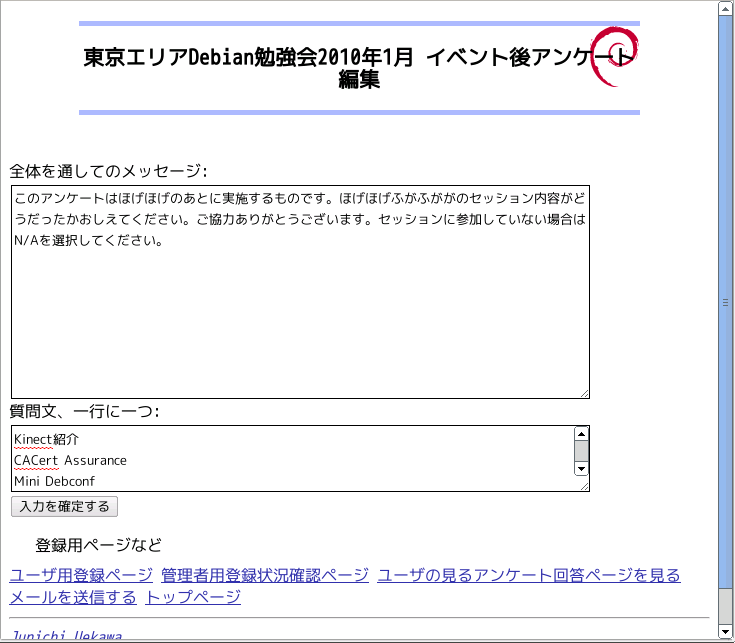
\includegraphics[width=1\hsize]{image201101/enquete-edit.png}
  \caption{アンケート編集画面}
 \end{center}
\end{minipage}
\begin{minipage}{0.5\hsize}
 \begin{center}
  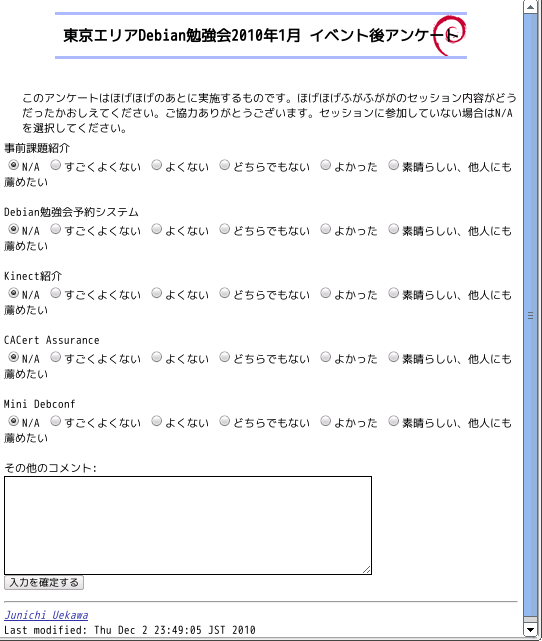
\includegraphics[width=1\hsize]{image201101/enquete-respond.png}
  \caption{アンケート回答画面}
 \end{center}
\end{minipage}
\end{figure}

\subsection{アンケートシステムの利用方法}

\subsubsection{管理者の事前準備}

イベントの管理者はイベントの一覧画面からアンケート作成画面に遷移すること
ができます。そこでは、ユーザに表示するための全体的なメッセージと、各項目
を改行区切りで記述する欄があります。

ユーザにメールを送信すると、ユーザにはリンクの書いてあるメールが届きます。
そのリンクをクリックすると、ユーザはアンケートに回答することができます。

\subsubsection{ユーザ}

ユーザは各項目については0から5までの値で回答することができます。
そして、全体について自由記述の項目があります。
\footnote{勉強会の会場では5択だと中心に回答が偏りがちなので、
4択にしたほうがよいのではないかという意見が出ました。Debian勉強会アンケー
トシステムでは中心に偏り過ぎているとい傾向はまだ出ていないのでこのまま進
めてみようと考えています。}

二つ目的があります。勉強会の企画の中で、どの部分が評価されているのかとい
うのを出していきたいのと、任意なメッセージを入力できるようにすることで会
に対してやりたいことなどの要望が伝えられるようにすることです。

\begin{table}[h]
 \caption{アンケート回答結果の内部表現}
 \begin{itemize}
  \item[0.] N/A \footnote{ユーザにとって回答に値しない、例えば自分がプレゼンテーション
	    していた場合や、遅刻・早退して自分がその場にいなかった、など、ア
	    ンケートに回答できない理由はいろいろありえます。}
  \item[1.] すごくよくない
  \item[2.] よくない
  \item[3.] どちらでもない
  \item[4.] よかった
  \item[5.] 素晴らしい、他人にも薦めたい
 \end{itemize}
\end{table}

\subsubsection{管理者が事後に確認}

管理者は、アンケートの[アンケート集計CSV]リンクをたどることにより、イベ
ント単位のデータのCSVダンプを見ることができます。

特に集計処理はしていません。ここから先はCSVをとりだして処理することにな
ります。

ここで、アンケートが匿名であるべきか記名であるべきかを最初考えていません
でした。どちらがどういう効果があるのかよくわかっていないので今後の課題と
したいと思います。ブログ代わりなのであれば記名でよいと思うのですが、アン
ケートが記名だとバイアスがかかるというのであれば匿名のほうがよいかもしれ
ません。システム的には今は匿名として扱っています。\footnote{Debian勉強会
の会場での議論では、回答の匿名性については。参加者のアンケート回答は匿名
扱いにしたほうが答えにバイアスがかかりにくいだろうという意見が出ました。}

\subsection{アンケートシステムの設計と実装}
\index{Google App Engine SDK}

アンケートシステムの設計と実装について見てみましょう。アンケートはDebian
勉強会予約システム\cite{deb201002debianreserve}の一機能として実装していま
す。

\subsubsection{データストア}

ここの設計で悩んだ点は、EventEnqueteResponseをAttendanceと一緒にするべき
かどうかです。Datastore がjoinをサポートしていないためです。今回は分離し
て必要なときに手動でjoin\footnote{同じキーで二回別のテーブルをqueryするこ
とになるので必要なときには効率が悪いけど、あまり必要にならないと予想した
設計}するアプローチにしてみました。

\begin{commandline}
class EventEnquete(db.Model):
    """Enquete questions for an event."""
    eventid = db.StringProperty()
    overall_message = db.TextProperty()
    question_text = db.StringListProperty()
    timestamp = db.DateTimeProperty(auto_now_add=True)

class EventEnqueteResponse(db.Model):
    """Enquete respnose for an event by one person."""
    eventid = db.StringProperty()
    # responses for 1-5 questions. 0 is N/A
    question_response = db.ListProperty(long)
    overall_comment = db.TextProperty() # a general comment from user.
    timestamp = db.DateTimeProperty(auto_now_add=True)
    user = db.UserProperty()
\end{commandline}

\subsubsection{ユーザインタフェース}

ユーザインタフェース部分は enquete.py に記述しています。メールやHTMLファ
イルの表示部分には、Django のテンプレートを利用しています。

\begin{itemize}
 \item EnqueteAdminEdit.html 管理者用のアンケート編集画面
 \item EnqueteAdminSendMail.txt 管理者が参加者にアンケートを依頼するメー
       ル送信するときのメールのテンプレート
 \item EnqueteAdminShowEnqueteResult.txt アンケートの結果をCSV形式で表示
       する。
 \item EnqueteRespond.html 参加者がアンケートを返答する際に表示される
       HTML。
 \item EnqueteRespondDone.txt 参加者がアンケートを回答したときに送信され
       る確認メール。
\end{itemize}

\subsubsection{バックグラウンドタスク}

ウェブインタフェースからアンケートの送信リクエストがあった場合、
クリックした瞬間にメールの送信処理が発生するわけではなく、
メールの送信処理にtaskqueueを利用しています。

送信元は noreply@debianmeeting.appspotmail.com を使っています。多分ログイ
ンユーザの権限でメールを出すということができないのだと想定してこうなって
います\footnote{未確認}。

\subsection{先月のアンケート集計結果}
\index{R}

それでは、例として2010年12月のアンケート結果をみてみましょう。
0は欠損値なので、Rに処理させる場合は「NA」として処理します。
これでRで処理した結果を見てみましょう。
まだこの時点ではデータが少ないので、今回のなかでどのセッションが
比較的ポジティブな感想を集めたのかということが分かるだけです。

事前準備として、統計解析ツールR\cite{r2008}をインストールします。ここでは
基本パッケージのr-baseとドキュメントのr-doc-info\footnote{R ではなにかわ
からないことがあればとりあえずinfoを見るか、help()コマンドをつかえばよい
かんじです。}をインストールしています。\index{r-base} \index{r-doc-info}

\begin{commandline}
# apt-get install r-base r-doc-info
\end{commandline}
\index{r-base}

R を起動してCSVファイルをロードして、まず基本的な統計量を調べます。

\begin{commandline}
$ R
[中略]
> enquete <- read.csv('201012enquete.csv')
> summary(enquete)
  事前課題紹介  X2010年のDebianを振り返って.2011年を企画する
 Min.   :3.00   Min.   :3
 1st Qu.:3.75   1st Qu.:3
 Median :4.00   Median :4
 Mean   :3.75   Mean   :4
 3rd Qu.:4.00   3rd Qu.:5
 Max.   :4.00   Max.   :5
 NA's   :1.00   NA's   :1
 CACertの準備に何が必要か 俺のlibsaneが火をふくぜ Debian.Miniconf.企画
 Min.   :4.000            Min.   :4.000           Min.   :1.000
 1st Qu.:4.000            1st Qu.:4.500           1st Qu.:2.000
 Median :5.000            Median :5.000           Median :3.000
 Mean   :4.556            Mean   :4.714           Mean   :2.778
 3rd Qu.:5.000            3rd Qu.:5.000           3rd Qu.:4.000
 Max.   :5.000            Max.   :5.000           Max.   :4.000
                          NA's   :2.000
> quantile(enquete$俺の, na.rm=TRUE)
  0%  25%  50%  75% 100%
 4.0  4.5  5.0  5.0  5.0
> quantile(enquete$Debian)
  0%  25%  50%  75% 100%
   1    2    3    4    4
\end{commandline}

ざっと数字を眺めただけですが、今回特に評価の高かったセッションはsaneネ
タと、CACertネタで、評価の低かったセッションはDebian Miniconf企画ネタでし
た。今回のアンケートの結果を受けると、Debian miniconfについてはプレゼンテー
ションの方法を考え直した方がよいだろうと思います。事前課題資料が無かった、
プレゼンテーションしようとしたマシンがプロジェクタにうまくつながらなかっ
た、そもそも話の内容もあまり練られていなかったということを考えるとそれが
そのままアンケートの統計値にも反映したと考えられます。

一つ目線を変えて相関を調べてみました。
しかし、まだこれをどう判断するべきか考えがまとまっていません。

\begin{commandline}
> cor(enquete$CAC, enquete$俺の, use="complete.obs")
[1] 0.7302967
> cor(enquete$俺の, enquete$事前, use="complete.obs")
[1] -0.2581989
> cor(enquete$CAC, enquete$事前, use="complete.obs")
[1] 0
\end{commandline}

また、勉強会で議論した結果出てきた懸念点としては、点数のフィードバックは
毎回出てこられても講師のやる気がそがれるなどの悪影響がある可能性がある点
でした。講師には一年に一回程度まとめて返すのがよいだろうという提案があり
ました。

\begin{thebibliography}{0}
 \bibitem{deb201012annualreport} 上川純一, 「2010年の東京エリアDebian勉強会をふりかえって」
東京エリアDebian勉強会 Deb専 2010年12月号
 \bibitem{deb201002debianreserve} 上川純一, 「東京エリアDebian勉強会予約システムの構想」
東京エリアDebian勉強会 Deb専 2010年2月号
\bibitem{r2008} R Development Core Team, ``R: A Language and
	Environment for Statistical Computing'', R Foundation for
	Statistical Computing, Vienna, Austria, 2008
	\url{http://www.R-project.org}
\end{thebibliography}

%-------------------------------------------------------------------------------
\dancersection{2010年の東京エリアDebian勉強会をふりかえって}{上川 純一}
%-------------------------------------------------------------------------------
\index{debianjp@Debian JP}
\index{とうきょうえりあ@東京エリアDebian勉強会}
\index{2010ねん@2010年}

今月で6年目のDebian勉強会が終了しました。
Debian Developer の数も着々と増えていき、当初の目標が達成されてきていま
すね。

今年東京エリアDebian勉強会常連のやまねさんがDebian Developerになりました。
苦節6年おめでとうございます。

Debian Maintainer 申請も複数通りました。

\subsection{基本的な数値}

Debian 勉強会は毎回事前課題事後課題を設定しており、予習復習を必要だとう
たっている勉強会です。
実際にどれくらいの人が出席しているのか、またその人たちがどれくらい事前課
題・事後課題を提出しているのか、確認してみましょう。
\fgref{fig:attendandprepostwork}です。
値は一年の移動平均です。

結果を見ると事前課題の提出率が2009年に低下傾向にあったのが、2010年に反転
上昇しています。これはDebian勉強会予約システムの導入により事前課題の提出
が簡単になったことと関係ありそうです。また、別の傾向として事後課題(ブロ
グ)の率が低下傾向にあります。もうブログは流行らないのかもしれません。


\begin{figure}[h]
 \begin{center}
 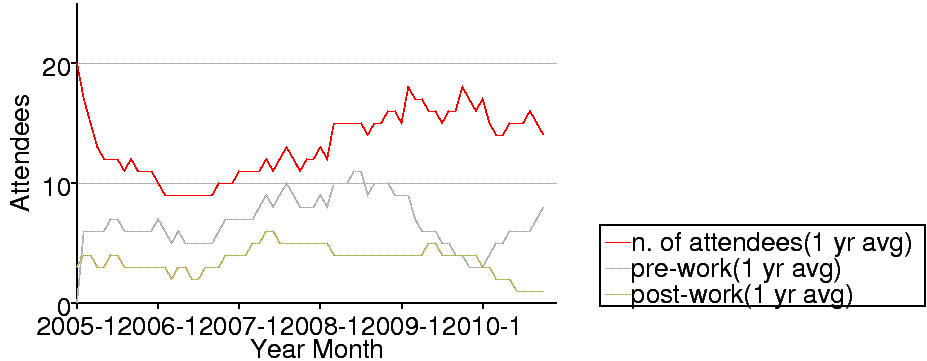
\includegraphics[width=1\hsize]{image201012/memberanalysis/attend.png}
 \end{center}
\caption{東京エリアDebian勉強会事前課題・事後課題提出実績(12ヶ月移動平均)}\label{fig:attendandprepostwork}
\end{figure}

毎回の参加者の人数と、その際のトピックを見てみます。今年はとくに目立った
感じの回はないですが、参加者についての記録が散逸しているようです。

今年の会場ですが、東京大学、筑波大学、木更津高専とアカデミックな場所の利
用が増えました。
\footnote{OSC も明星大学で開催されました}。また、NIFTYさんの会場も使い、
公営の会議室(杉並区、オリンピックセンターなど)は数回しか利用していません。

\begin{table}[H]
\begin{minipage}{0.5\hsize}
 \caption{東京エリアDebian勉強会参加人数(2005-2006年)}\label{tab:count}
 \begin{center}
  \begin{tabular}{|l|c|p{10em}|}
 \hline
   & 参加人数 & 内容 \\
 \hline
   2005年1月 & 21 & 秘密\\
   2005年2月 & 10 & debhelper 1\\
   2005年3月 & 8 &  (早朝) debhelper 2、social contract\\
   2005年4月 & 6 & debhelper 3\\
   2005年5月 & 8 & DFSG、dpkg-cross、lintian/linda\\
   2005年6月 & 12 & alternatives、d-i\\
   2005年7月 & 12 & toolchain、dpatch\\
   2005年8月 & 7 & Debconf参加報告、ITPからアップロードまで\\
   2005年9月 & 14 & debconf\\
   2005年10月 & 9 & apt-listbugs、バグレポート、debconf翻訳、debbugs\\
   2005年11月 & 8 & DWN翻訳フロー、statoverride\\
   2005年12月 & 8 & 忘年会\\
   2006年1月 & 8 & policy、Debian勉強会でやりたいこと\\
   2006年2月 & 7 & policy、multimedia \\
   2006年3月 & 30 & OSC: debian勉強会、sid \\
   2006年4月 & 15 & policy、\LaTeX{} \\
   2006年5月 & 6 & mexico \\
   2006年6月 & 16 & debconf、cowdancer\\
   2006年7月 & 40 & OSC-Do: MacBook Debian \\
   2006年8月 & 17 & 13執念 \\
   2006年9月 & 12 & 翻訳、Debian-specific、oprofile \\
   2006年10月 & 23 & network、i18n会議、Flash、apt \\
   2006年11月 & 20 & 関西開催: bug、sid、packaging \\
   2006年12月 & 14 & 忘年会 \\
 \hline
  \end{tabular}
 \end{center}
\end{minipage}
\begin{minipage}{0.5\hsize}
 \caption{東京エリアDebian勉強会参加人数(2007-2008年)}\label{tab:count2007}
 \begin{center}
  \begin{tabular}{|l|c|p{10em}|}
 \hline
 & 参加人数 & 内容\\
 \hline
   2007年1月 & 15 & 一年を企画する \\
   2007年2月 & 13 & dbs, dpatch\\
   2007年3月 & 80 & OSC仮想化 \\
   2007年4月 & 19 & quilt, darcs, git\\
   2007年5月 & 23 & etch, pbuilder, superh \\
   2007年6月 & 4 & エジンバラ開催:Debconf7 実況中継 \\
   2007年7月 & 18 & Debconf7 参加報告\\
   2007年8月 & 25 & cdn.debian.or.jp \\
   2007年9月 & 14 & exim \\
   2007年10月 & 30 & OSC Tokyo/Fall(CUPS) \\
   2007年11月 & 19 & live-helper, tomoyo linux kernel patch, server\\
   2007年12月 & 11 & 忘年会\\
   2008年1月 & 23 & 一年を企画する \\
   2008年2/29,3/1 & 36 & OSC  \\
   2008年3月 & 37 & データだけのパッケージ、ライセンス \\
   2008年4月 & 17 & バイナリパッケージ \\
   2008年5月 & 20 & 複数のバイナリパッケージ \\
   2008年6月 & 10 & debhelper \\
   2008年7月 & 17 & Linux kernel patch / module パッケージ \\
   2008年8月 & 10 & Debconf IRC会議とDebian温泉 \\
   2008年9月 & 17 & po4a, 「Debian メンテナのお仕事」 \\
   2008年10月 & 11? & OSC Tokyo/Fall \\
   2008年11月 & 17 & 「その場で勉強会資料を作成しちゃえ」 Debian を使った \LaTeX{} 原稿作成合宿 \\
   2008年12月 & 12 & 忘年会 \\
 \hline
  \end{tabular}
 \end{center}
\end{minipage}
\end{table}

\begin{table}[H]
\begin{minipage}{0.5\hsize}
 \caption{東京エリアDebian勉強会参加人数(2009-2010年)}\label{tab:count2009}
 \begin{center}
  \begin{tabular}{|l|c|p{10em}|}
 \hline
 & 参加人数 & 内容\\
 \hline
   2009年1月 & 12 & 一年を企画する \\
   2009年2月 & 30 & OSC パッケージハンズオン\\
   2009年3月 & 23 & Common Lisp, パッケージ作成 \\
   2009年4月 & 15 & Java Policy, ocaml, 開発ワークフロー\\
   2009年5月 & 13 & MC-MPIパッケージ化、Erlang、Androidアプリ、DDTP \\
   2009年6月 & 14 & DDTP・DDTSS、bsdstatsパッケージ、Debian kFreeBSD\\
   2009年7月 & 4 & スペインにてDebconf 9\\
   2009年8月 & 14 & スペイン Debconf 9 参加報告 \\
   2009年9月 & 26 & GPGキーサインパーティー \\
   2009年10月 & 30 & OSC Tokyo Fall\\
   2009年11月 & 12 & Octave, R, gnuplot, auto-builder \\
   2009年12月 & 10 & 忘年会\\
   2010年1月 & 17 &  東京大学にて新年会 \\
   2010年2月 & 11 & Debian温泉,ocaml,haskell \\
   2010年3月 & 12 & weka,fftw,dpkg v3 quilt \\
   2010年4月 & 15 & upstart,piuparts,debtags \\
   2010年5月 & 22 & 筑波大学,kernel \\
   2010年6月 & 12 & OSC-Doリハーサル  \\
   2010年7月 & 0 & キャンセル  \\
   2010年8月 & 3 & Debconf (NYC) \\
   2010年9月 & 30 & OSC Tokyo/Fall \\
   2010年10月 & 13 & 俺のDebianな一日 \\
   2010年11月 & 15 & ext4,btrfs,nilfs,ceph \\
   2010年12月 & 14 &  cacert, libsane \\
 \hline
  \end{tabular}
 \end{center}
\end{minipage}
\end{table}

%-------------------------------------------------------------------------------
\dancersection{関西 Debian 勉強会 2010年度各種イベント開催実績と総括}{倉敷・佐々木・野方}
%-------------------------------------------------------------------------------
\index{かんさいでびあん@関西Debian勉強会}
\index{2010ねん@2010年}
\subsection{運営状況}

\subsubsection{勉強会全体}

毎月のセッションについてですが、 %
勉強会の常連さんやイベント等で交流のある方に講師を依頼したりすることで、 %
参加者が関心を持っている様々な分野のネタを勉強会で行なう事ができました。
その反面 Debian との関連性に薄いネタが増えている、という指摘も受けています
\footnote{ネタ自体は Debian に絡められるのに, あんまり関連性について触れられていない, 等}。%
これは我々運営側が講師に依頼する際にもっと明確にお願いすべき事柄の様な気もします。%
今後の反省材料としたい所です。
また、今回の事前課題で複数の方が提出されている通り、%
定番のネタ(Debian 入門的なお話やライセンス、パッケージ作成等)を%
雑誌のように毎年繰り返すことも考えてみたい所です。

講師については、%
継続して参加者して下さる常連さんへの講師依頼をする中で、%
その方が勉強会の運営側へ参加して下さったり、という嬉しい事もありました。
また、Ubuntu コミュニティとの交流があったり、という感じでした。
人の輪がこうして広がっていくのは嬉しいですね。

事前課題については、%
「Debian 勉強会登録システム」の実装と連動してシステム化されたこともあり、%
関西でも毎回の流れにのってきました。%
来年からは東京のように統計をとってもいいかな、と考えています。

イベント参加については、%
今年は春先に OSC Kobe が開催されたため、%
年間通して 3 回分をイベントセッションという形で実施しました。
%
また、勉強会から fork (?) する形でGPG キーサインパーティの実施も定例となりつつあります。
来年も今年通り 3 回の参加を予定しておりますが、%
takaya さんより「ユーザ向け」と「開発者(含むワナビー)向け」の 2 セッションに分けたらどうか、%
との提案もあったりしています。%
当面 4 月の OSC Kobe でのお話になりますが、検討してみたい所です%
\footnote{人的リソースやそもそも二枠取れるのか, 等と気になる課題はありますが}。

{\tt{debian.org}} については、
今年度は佐々木、倉敷の 2 名がめでたく Debian Maintainer になりました。
来年もこの流れを維持できればと思います。

\subsubsection{イベント関連}

例年通り、夏のオープンソースカンファレンスKansai@Kyoto(OSC京都)と、秋の関
西オープンフォーラム(KOF)の出展にくわえ、3月に神戸で開催されたオープンソー
スカンファレンスKansai@Kobe(OSC神戸)にも参加しました。

そしてOSC京都とKOFでは、佐々木さんが中心となりGPGキーサインパーティを開催
しました。

セッションの内容については、OSC神戸やKOFでは最近のDebian関連情報を伝える
軽めのセッション、OSC京都ではパッケージのバックポート講座を開きましたが、
情報系より手を動かすセッションのほうが反響があったので、ハンズオン的なこ
とを増やしていければと思います。

イベントについてはFLOSS関連のイベントが年2回から3回に増えたことと、GPGキー
サインパーティの担当、イベント側のスタッフとして参加など、リソースが若干
厳しくなってきたのでなにかいいバランスを取ることを考えたほうがいいのかも
しれません。


\subsection{開催実績}

関西Debian勉強会の出席状況を確認してみましょう。
グラフで見ると\fgref{fig:kansaipeoplechart}になります。
表で見ると\tbref{tab:count2010kansai} です。

\begin{figure}[h]
 \begin{center}
  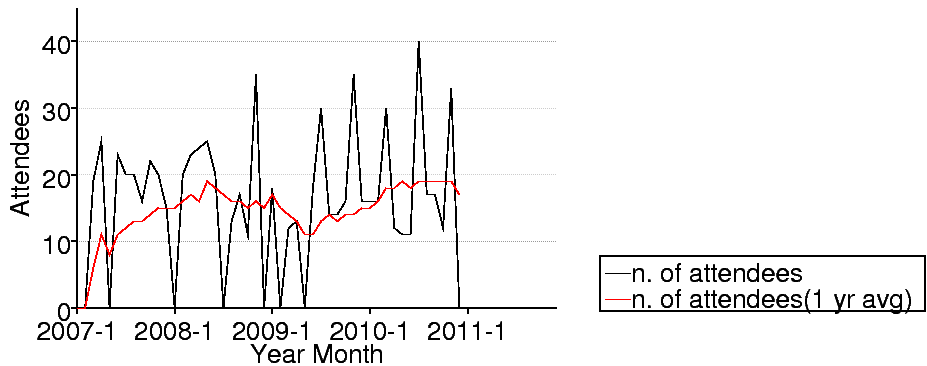
\includegraphics[width=1\hsize]{image201012/memberanalysis/kansai.png}
 \end{center}
\caption{関西の参加人数推移}
\label{fig:kansaipeoplechart}
\end{figure}

\begin{table}[H]
\begin{minipage}{0.5\hsize}
 \caption{関西Debian勉強会参加人数(2007年)}\label{tab:count2007kansai}
 \begin{center}
  \begin{tabular}{|l|c|p{10em}|}
 \hline
 & 参加人数 & 内容 \\
 \hline
2007年3月 & 19 & 開催にあたり \\
2007年4月 & 25 & goodbye、youtube、プロジェクトトラッカー\\
2007年6月 & 23 & 社会契約、テーマ、debian/rules、bugreport\\
2007年7月 & 20前後 & OSC-Kansai \\
2007年8月 & 20 & Inkscape、patch、dpatch\\
2007年9月 & 16 & ライブラリ、翻訳、debtorrent\\
2007年10月 & 22& 日本語入力、SPAMフィルタ\\
2007年11月 & 20前後 & KOF \\
2007年12月 & 15& 忘年会、iPod touch\\
 \hline
  \end{tabular}
 \end{center}
\end{minipage}
\begin{minipage}{0.5\hsize}
 \caption{関西Debian勉強会参加人数(2008年)}\label{tab:count2008kansai}
 \begin{center}
  \begin{tabular}{|l|c|p{10em}|}
 \hline
 & 参加人数 & 内容 \\
 \hline
2008年2月 & 20 & PC Cluster, GIS, \TeX \\
2008年3月 & 23 & bug report, developer corner, GPG \\
2008年4月 & 24 & coLinux, Debian GNU/kFreeBSD, sid \\
2008年5月 & 25  & ipv6, emacs, ustream.tv\\
2008年6月 & 20  & pbuilder, hotplug, ssl\\
2008年8月 & 13  & coLinux \\
2008年9月 & 17  & debian mentors, ubiquity, DFSG\\
2008年10月 & 11  & cdbs,cdn.debian.or.jp \\
2008年11月 & 35  & KOF \\
2008年12月 & ?  & TeX資料作成ハンズオン\\
 \hline
  \end{tabular}
 \end{center}
\end{minipage}
\begin{minipage}{0.5\hsize}
 \caption{関西Debian勉強会参加人数(2009年)}\label{tab:count2009kansai}
 \begin{center}
  \begin{tabular}{|l|c|p{10em}|}
 \hline
 & 参加人数 & 内容 \\
 \hline
2009年1月 & 18 & DMCK, LT \\
2009年3月 & 12 & Git \\
2009年4月 & 13 & Installing sid, Mancoosi, keysign \\
2009年6月 & 18 & Debian Live, bash\\
2009年7月 & 30? & OSC2009Kansai \\
2009年8月 & 14 & DDTSS, lintian \\
2009年9月 & 14 & reportbug, debian mentors\\
2009年10月 & 16 & gdb, packaging \\
2009年11月 & 35 & KOF2009 \\
2009年12月 & 16 & GPS program, OpenStreetMap \\
 \hline
  \end{tabular}
 \end{center}
\end{minipage}
\begin{minipage}{0.5\hsize}
 \caption{関西Debian勉強会参加人数(2010年)}\label{tab:count2010kansai}
 \begin{center}
  \begin{tabular}{|l|c|p{10em}|}
 \hline
 & 参加人数 & 内容 \\
 \hline
2010年1月 & 16 & Xen, 2010年企画 \\
2010年2月 & 16 & レンタルサーバでの利用, GAE \\
2010年3月 & 30? & OSC2010Kobe \\
2010年4月 & 12 & デスクトップ環境, 正規表現 \\
2010年5月 & 11 & ubuntu, squeeze \\
2010年6月 & 11 & debhelper7, cdbs, puppet \\
2010年7月 & 40? & OSC2010Kyoto \\
2010年8月 & 17 & emdebian, kFreeBSD \\
2010年9月 & 17 & タイルWM \\
2010年10月 & 12 & initramfs, debian live \\
2010年11月 & 33 & KOF2010 \\
2010年12月 & 14 & Proxmox, annual review \\
 \hline
  \end{tabular}
 \end{center}
\end{minipage}
\end{table}

\newpage

\dancersection{執筆者紹介}{}

本号の執筆に参加したメンバを紹介します。
\begin{multicols}{2}
 \begin{description}
  \item[本庄 弘典]
             必要に迫られ自宅の本を自炊。焼き鳥が好き。
  \item[山田 泰資]
	     Debian JP Project Member。Debian JP 副会長。
             DDになって自分のソフトをパッケージ化して世界征服するのが野
	     望。これでまた野望に一歩近づいた・・・?
  \item[野島 貴英]
	     昔Debianを使って稼いだ経験から、Contribution生活に憧れる。
             しかしその実態は、典型IT土方生活との折り合いをなんとか付けようと日々もがくチキン野郎。
  \item[まえだ こうへい]
             Debian JP Project Member。Debian JP 会長。
             あまり人の使わないマイノリティな技術をDebianで使って、
             愛猫こまめとヨメとの生活をいかに楽にできるかに腐心してる。
  \item[岩松 信洋]
             Debian Project Member (Debian Developer)。東京エリア Debian 勉強会から輩出され
             た Debian Developer1号。子供の影響で鉄分(鉄道)を多く摂取するようになった。
  \item[山本 浩之]
	     Debian JP Project Member。
             PPC64 をDebian にポーティングする日々を過ごす休日プログラマ。
% HACK HACK: insert space to make the split better here
\\
\\
  \item[上川 純一]
	     Debian Project Member (Debian Developer)、 東京エリア Debian 勉強会創始者。
	     印刷物の完成を眺めるのが結構すき。
  \item[森山 京平]
             NAIST(奈良の森の中の大学院)にいる Ubuntu User。
  \item[杉本 典充]
	     北海道、関西、東京といろいろな土地で開催する Debian 勉強会に出没する道民。
	     主に Debian GNU/kFreeBSD を使い unstable の醍醐味に浸る日々を過ごしている。
  \item[のがた じゅん]
	     Debian Live をこよなく愛す、38歳無職ニートヒッキーパンクロッカー。 
  \item[水野 源]
	     理想のビールを求めて西へ東へ。最近はサッポロクラシックがフェイバリット。
	     Ubuntu Japanese Team 所属。
  \item[倉敷 悟]
	     Debian Maintainer と翻訳で修行している、Debian Developer ワナビー。
             puppet 楽しいよ puppet。
  \item[かわだ てつたろう] Debian のドキュメント周りに興味がある関西在住の Debian User。
  \item[木下 達也]
	     Debian Project Member (Debian Developer)。
	     Wanderlust, Mew, w3m のメンテナ。
  \item[山下 康成]
             LinkStation/玄箱 を中心にいろいろいじっている人。 
 \end{description}
\end{multicols}

% FIXME: quizを追加すること
\dancersection{Debian Trivia Quiz}{上川 純一}

ところで、みなさん Debian 関連の話題においついていますか?Debian関連の話
題はメーリングリストをよんでいると追跡できます。ただよんでいるだけではは
りあいがないので、理解度のテストをします。特に一人だけでは意味がわからな
いところもあるかも知れません。みんなで一緒に読んでみましょう。


\begin{multicols}{2}
 %; whizzy-master ../debianmeetingresume2011-natsu.tex
% $B0J>e$N@_Dj$r$7$F$$$k$?$a!"$3$N%U%!%$%k$G(B M-x whizzytex $B$9$k$H!"(Bwhizzytex$B$,MxMQ$G$-$^$9!#(B
%
% $B$A$J$_$K!"%/%$%:$OJL%V%i%s%A$G:n@.$7!"$N$A$K%^!<%8$7$^$9!#5U$K%^!<%8$7(B
% $B$J$$$h$&$K$7$^$7$g$&!#(B
% (shell-command "git checkout quiz-prepare")

\santaku
{DACA $B$C$F$J$s$G$9$+(B?}
{Debian Admin Coaching Association}
{Debian $B$r;H$&$H(B (A)$B$"$N;R$H(B (C)$B%/%j%9%^%9$K(B (A)$B%"%l$,$G$-$k$+$b$7$l$J$$(B}
{Debian's Automated Code Analysi project}
{C}
{$B2r@b(B}

\santaku
{DebConf11 $B$O$$$D3+:E$5$l$k$G$7$g$&(B}
{2011/6/24 - 30}
{2011/7/24 - 30}
{2011/8/24 - 30}
{B}
{$B2r@b(B}

\santaku
{squeeze $B$N(B Linux $B%+!<%M%k$O0lL#0c$$$^$9!#2?$,0c$&$G$7$g$&!#(B}
{non-free firmware $B$rGS=|$7$?(B}
{Tux $B$/$s$rGS=|$7$?(B}
{$B0l$D$N%+!<%M%k%$%a!<%8$G(BkFreeBSD$B$H(BLinux$B$rDs6!$7$^$9(B}
{A}
{$B2r@b(B}

\santaku
{2010/12/17 $B$N;~E@$G(BRC$B%O%0$O$$$/$D$"$k$G$7$g$&!#(B}
{3} 
{83}
{183}
{C}
{$B2r@b(B}

\santaku
{New Maintianer $B%U%m%s%H%G%9%/$KDI2C$5$l$?%a%s%P!<$O!)(B}
{Xavier Oswald}
{Enrico Zini}
{Kenshi Muto}
{A}
{$B2r@b(B}

\santaku
{RC$B%P%0$N8=>u$O$O$I$3$G3NG'$G$-$k$+(B}
{\url{http://bugs.debian.org/release-critical/}}
{\url{http://localhost/}}
{\url{http://debianmeeting.appspot.com/}}
{A}
{$B2r@b(B}

\santaku
{Debian$BJY6/2qM=Ls%7%9%F%`$N(BURL$B$O$I$l$+(B}
{\url{http://www.2ch.net/}}
{\url{http://atnd.org/events/}}
{\url{http://debianmeeting.appspot.com/}}
{C}
{$B2r@b(B}

\santaku
{events@debian.org$B$O$I$3$HE}9g$5$l$?$+(B}
{merchants@debian.org}
{hoge@debian.org}
{fuga@debin.org}
{A}
{$B2r@b(B}

\santaku
{antiharassment@debian.org $B$N$&$i$K$$$J$$$N$OC/$+(B}
{Amaya Rodrigo Sastre}
{Patty Langasek}
{Kouhei Maeda}
{C}
{$B2r@b(B}

\santaku
{$B8=:_$$$/$D$+$N(BSprint$B$,3+:E$5$l!"4k2h$5$l$F$$$k!#8=:_4k2h$9$i$5$l$F$$$J(B
$B$$(Bsprint$B$O$I$l$+(B}
{-www sprint}
{security sprint}
{tokyo sprint}
{C}
{$B2r@b(B}

\santaku
{DACA$B$O$I$3$r8+$l$P$h$$$+(B}
{\url{http://qa.debian.org/daca/}}
{\url{http://daca.debian.org/}}
{\url{file:/tmp}}
{A}
{$B2r@b(B}

\santaku
{DEP $B$O2?$NN,$+(B}
{Debian Enhancement Proposal}
{Device Enhancement Protocol}
{$B$G$C$W(B}
{A}
{$B2r@b(B}

\santaku
{DEP5$B$GDs0F$5$l$F$$$k(Bdebian/copyright$B$N5!3#2DFI7A<0$O$I$&$$$&$b$N$+(B}
{S$B<0(B}
{RFC822$BIw(B}
{XML}
{B}
{$B2r@b(B}

\santaku
{Debian 6.0 $B$,%j%j!<%9$5$l$?$N$O$$$D$+!)(B}
{2011/02/05}
{2011/02/06}
{2011/02/07}
{A}
{$B2r@b(B}

\santaku
{$B:#2s$N%j%j!<%9$G%5%]!<%H$5$l$J$/$J$C$?%"!<%-%F%/%A%c$O!)(B}
{m68k, ppc64}
{alpha, arm, hppa}
{blackfin, microblaze}
{B}
{$B2r@b(B}

\santaku
{www.debian.org $B$N%G%6%$%s$,JQ99$5$l$^$7$?!#2?G/F1$8%G%6%$%s$r;H$C$F$$$?$+!)(B}
{11$BG/(B}
{12$BG/(B}
{13$BG/(B}
{C}
{$B2r@b(B}

\santaku
{$B<!$N%j%j!<%9%3!<%I%M!<%`$O2?$+!)(B}
{rc}
{spell} % Mr.Spell
{wheezy}
{C}
{$B2r@b(B}

\santaku
{$B:#EY9T$o$l$k(BFTP-master$B2q5D$G5DO@$5$l$J$$M=Dj$O!)(B}
{$B%Q%C%1!<%8<+F0%5%$%s5!9=(B}
{$B%/%m%9%3%s%Q%$%k%5%]!<%H(B}
{md5sum$B$H(BshaXsum$B$r$H$C$Q$i$&(B}
{B}
{$B2r@b(B}

\santaku
{Lars Wirzenius$B$,Ds0F$7$?<!$N%j%j!<%9%4!<%kL\I8$O!)(B}
{UTF-8$B$GF0$+$J$$%Q%C%1!<%8$r$J$/$9(B}
{Debian$B$GF0$$$F$$$k?M9)1R@1$rBG$A>e$2$^$9(B}
{$BA4%Q%C%1!<%8$r(BLLVM$B$G%S%k%I$7$^$9(B}
{A}
{$B2r@b(B}

\santaku
{2011$BG/EY(B Debian JP $B2qD9$OC/$G$7$g$&$+!)(B}
{$BA0ED(B $B9LJ?(B}
{$B4d>>(B $B?.MN(B}
{$B9SLZ(B $BLw9((B}
{A}
{$B2r@b(B}

\santaku
{2011$BG/EY(B DPL $B$OC/$G$7$g$&$+!)(B}
{Kurt Roeckx}
{Kenshi Muto}
{Stefano Zacchiroli}
{C}
{$B2r@b(B}

\santaku
{Debian Policy 3.9.2 $B$GDI2C$5$l$F$$$J$$9`L\$O$I$l$+(B}
{Debian$B%"%+%&%s%H$r%a%s%F%J%"%I%l%9$KDI2C$9$kI,MW$,$"$j$^$9!#(B}
{$B%"!<%-%F%/%A%c0MB8$N%i%$%V%i%jEy$O(B DEB\_HOST\_MULTIARCH $B$G<hF@$7$?CM$rMx(B
$BMQ$9$kI,MW$,$"$j$^$9!#(B}
{$BA4$F$N%Q%C%1!<%8$O(BVCS$B$G4IM}$9$kI,MW$,$"$j$^$9!#(B}
{C}
{$B2r@b(B}

\santaku
{DebConf chairs$B$K;XL>$5$l$?$N$OC/!)(B}
{Gunnar Wolf}
{Maeda Kouhei}
{Junichi Uekawa}
{A}
{$B2r@b(B}

\santaku
{ries.debian.org $B$G<hF@$G$-$k$h$&$K$J$C$?%G!<%?$O!)(B}
{debian.org $B$N2TF/>u67%G!<%?(B}
{debian.org $B$N(BML$B%G!<%?$r(Bgzip$B$G8G$a$?J*(B}
{dak $B$N%G!<%?(B}
{C}
{$B2r@b(B}

\santaku
{/run $B$,>C$5$l$?M}M3$O!)(B}
{/go $B$N$[$&$,$h$/$M!)$H$$$&?M$,8=$l$?!#(B}
{initscripts $B$,$^$@%5%]!<%H$7$F$J$$!*(B}
{/run $B$rF~$l$?$N$O%Q%C%1!<%8%s%0%_%9$G$9!#(B}
{B}
{$B2r@b(B}

\santaku
{HPPA $B$H(B alpha $B$N0\E>@h$O$I$3$G$7$g$&$+!)(B}
{buildd.debian.or.jp}
{buildd.debian-ports.org}
{www.buildd.net}
{B}
{$B2r@b(B}

\santaku
{linux$B%+!<%M%k(B 2.6.39$B$,(BDebian$B$KF~$k$3$H$K$h$C$F5/$-$kJQ99$O!)(B}
{i386-bigmem$B$,(Bi386-pae$B$K$J$C$?(B}
{amd64$B$,(Bi386$B$K$J$C$?(B}
{i386$B$O(Bamd64$B$N%^%k%A%P%$%J%j$K$J$C$?(B}
{A}
{$B2r@b(B}

\santaku
{Qt3$B%Q%C%1!<%8$,:o=|$5$l$J$$M}M3$O!)(B}
{Qt3$B%f!<%6$K$h$k0%4j$N$?$a(B}
{LSB 4.1$B$,(BQt3$B$rI,MW$H$7$F$$$k$?$a(B}
{$B:o=|$N;EJ}$,$o$+$i$J$$(B}
{B}
{$B2r@b(B}

\santaku
{Debian$B$N%5!<%P$KDI2C$5$l$?5!G=$O!)(B}
{$B%m%0%$%s$7$F$$$k%f!<%6$r(BIRC$B$KN.$95!G=(B}
{RFC1149 $B$N<BAu(B}
{DNSSEC}
{C}
{$B2r@b(B}

\end{multicols}

% 問題と回答が同じみひらきにならないようにする
\cleartoevenpage
\dancersection{Debian Trivia Quiz 問題回答}{上川 純一}

 Debian Trivia Quiz の問題回答です。
 あなたは何問わかりましたか?
 \\
 %回答はdebianmeetingresume2010-natsu.jqzというファイルに生成されるので、
 %それを手動でコピペして使う。
 % ここからコピペ
 % FIXME 問題が全部はいったらコピペすること
 %(progn (next-line 1)(insert-file "debianmeetingresume2011-natsu.jqz") )
1. C\\
2. B\\
3. A\\
4. C\\
5. A\\
6. A\\
7. C\\
8. A\\
9. C\\
10. C\\
11. A\\
12. A\\
13. B\\
14. A\\
15. B\\
16. C\\
17. C\\
18. B\\
19. A\\
20. A\\
21. C\\
22. C\\
23. A\\
24. C\\
25. B\\
26. B\\
27. A\\
28. B\\
29. C\\

%-------------------------------------------------------------------------------------
%% Footer
%-------------------------------------------------------------------------------------

\printindex

% add page to even number multiple of 4.
%\newpage
%\thispagestyle{empty}\mbox{}
\newpage
\thispagestyle{empty}\mbox{}%裏表紙の裏側のページ、色紙
\newpage
\cleartoevenpage

\thispagestyle{empty}
{
\large
\begin{itembox}{\bf 『あんどきゅめんてっど でびあん』について}
本書は、東京および関西周辺で毎月行なわれている『東京エリア Debian 勉強会』および
『関西エリア Debian 勉強会』で
使用された資料・小ネタ・必殺技などを一冊にまとめたものです。
収録範囲は東京エリアは2010年12月勉強会(第71回)から2011年05月勉強会(第77回)、関西エリアは第42回から第47回 まで。
% FIXME: 回数を修正すること。
内容は無保証、つっこみなどがあれば勉強会にて。
\end{itembox}
}

\vspace*{15cm}
{\color{dancerlightblue}\rule{\hsize}{1mm}}
\vspace{2mm}

\includegraphics[width=2cm]{image200502/openlogo-nd.eps}
\noindent \Large \bf あんどきゅめんてっど でびあん 2011年夏号\\
\noindent \normalfont 2011年08月13日 \hspace{5mm}  初版第1刷発行\\
\noindent \normalfont 東京エリア Debian 勉強会/関西エリア Debian 勉強会 (編集・印刷・発行)\\
{\color{dancerdarkblue}\rule{\hsize}{1mm}}

\end{document}
